%\documentclass[a4paper,12pt,english,twoside,openright]{book}
\documentclass[english,12pt,booktabs,hyperref,titling,twoside,openright]{hepthesis}
%%% hepthesis requirements
\usepackage{setspace,fancyhdr,rotating,comment,tocbibind,changepage,varwidth,csquotes,babel,a4wide,amsmath,hyperref,booktabs,draftcopy,lineno}
%\usepackage[babel]{csquotes}
\usepackage{hepnames,hepunits,hepparticles}
\usepackage{epsfig,amssymb,latexsym,numprint,textcomp}
%\usepackage[utf8]{inputenc}
%\usepackage{appendix}
%\usepackage{epstopdf}
\usepackage{subfigure}
\usepackage{graphicx}
\usepackage{color}
\usepackage[backend=biber, sorting=none, citestyle=numeric-comp]{biblatex}
\usepackage[format=plain,labelfont=bf]{caption}
\usepackage{enumerate}
\usepackage{lscape}
\usepackage{emptypage}
\usepackage{pifont}
\usepackage{multirow}
\usepackage{tabularx}

\linenumbers
\parskip = 0pt

\graphicspath{/home/lviliani/Documenti/PhdThesis/images}
\let\oldMeV\MeV
\let\oldGeV\GeV
\let\oldTeV\TeV
\renewcommand{\MeV}{\,\oldMeV \xspace}
\renewcommand{\GeV}{\,\oldGeV \xspace}
\renewcommand{\TeV}{\,\oldTeV \xspace}
\newcommand{\hww}{\ensuremath{{\mathrm{H}\to\mathrm{WW}}}\xspace}
\newcommand{\hwwllnn}{\ensuremath{{\mathrm{H}\to\mathrm{WW}\to\mathrm{2\ell2\nu}}}\xspace}
\newcommand{\ttH}{\ensuremath{\mathrm{t\bar{t}H}}\xspace}
\newcommand{\fb}{\ensuremath{\mathrm{fb}}\xspace}
\newcommand{\pb}{\ensuremath{\mathrm{pb}}\xspace}
\newcommand{\ifb}{\ensuremath{\,\mathrm{fb^{-1}}}\xspace}
\newcommand{\ipb}{\ensuremath{\mathrm{pb^{-1}}}\xspace}
\newcommand{\WW}{\ensuremath{\mathrm{WW}}\xspace}
\newcommand{\W}{\ensuremath{\mathrm{W}}\xspace}
\newcommand{\F}{\ensuremath{\cmsSymbolFace{F}}}
\newcommand{\V}{\ensuremath{\cmsSymbolFace{V}}\xspace}
\newcommand{\VVV}{\cmsSymbolFace{VVV}\xspace}
\newcommand{\Wjets}{\ensuremath{\PW\text{+jets}}\xspace}
\newcommand{\X}{\ensuremath{\cmsSymbolFace{X}}\xspace}
\newcommand{\delphill}{\ensuremath{\Delta\phi_{\ell\ell}}}
\newcommand{\delphillmet}{\ensuremath{\Delta\phi(\ell\ell,\VEtmiss)}}
\newcommand{\dyll}{\ensuremath{Z/\gamma^*\to \ell^+\ell^-}\xspace}
\newcommand{\dymm}{\ensuremath{Z/\gamma^*\to\Pgmp\Pgmm}}
\newcommand{\dytt}{\ensuremath{Z/\gamma^* \to\tau^+\tau^-}}
\newcommand{\jp}{\ensuremath{J^{P}}\xspace}
\newcommand{\mll}{\ensuremath{m_{\ell\ell}}\xspace}
\newcommand{\mt}{\ensuremath{m_\mathrm{T}}\xspace}
\newcommand{\mti}{\ensuremath{m_\mathrm{T}^\mathrm{i}}\xspace}
\newcommand{\psvectorKD}{\ensuremath{\mathcal{D}_{1^-}}\xspace}
\newcommand{\ptl}{\ensuremath{p_\perp^{\ell}}\xspace}
\newcommand{\ptll}{\ensuremath{\pt^{\ell\ell}}\xspace}
\newcommand{\MET}{\ensuremath{E_\mathrm{T}^\mathrm{\,miss}}\xspace}
\newcommand{\ptmiss}{\ensuremath{\vec{p}_\mathrm{T}^\mathrm{\,miss}}\xspace}
\newcommand{\qq}{\ensuremath{\Pq\Pq}\xspace}
\newcommand{\superKD}{\ensuremath{\mathcal{D}_\text{bkg}} }
\newcommand{\tw}{\ensuremath{\cPqt\PW}\xspace}
\newcommand{\vectorKD}{\ensuremath{\mathcal{D}_{1^+}} }
\newcommand{\wgamma}{\ensuremath{\PW\gamma}\xspace}
\newcommand{\mjj}{\ensuremath{m_{jj}}\xspace}
\newcommand{\pt}{\ensuremath{p_\mathrm{T}}\xspace}
\newcommand{\pth}{\ensuremath{p_\mathrm{T}^\mathrm{H}}\xspace}
\newcommand{\ttbar}{\ensuremath{\mathrm{t}\bar{\mathrm{t}}}\xspace}
\newcommand{\jpb}{{\em JetBProbability }\xspace}
\newcommand{\tg}{{\em tag}\xspace}
\newcommand{\probe}{{\em probe}\xspace}
\newcommand{\tp}{{\em tag-probe}\xspace}
\newcommand{\tpp}{{\em tag-pass-probe}\xspace}
\newcommand{\tfp}{{\em tag-fail-probe}\xspace}


\pdfinfo{%
  /Title    (PhD Thesis)
  /Author   (Lorenzo Viliani)
}


\bibliography{PhDThesis}

\begin{document}

\setspacing{single}

\begin{frontmatter}

\title{Measurement of the Higgs boson transverse momentum spectrum in the WW decay channel at 8\,TeV and first results at 13\,TeV}
\author{Lorenzo Viliani}

\titlepage[of University of Florence]{PhD Thesis}

\begin{abstract}
The cross section for Higgs boson production in pp collisions is studied using the $\mathrm{H} \to \mathrm{W}^+ \mathrm{W}^-$  decay mode, followed by leptonic decays of the W bosons, leading to an oppositely charged electron-muon pair in the final state. 
The measurements are performed using data collected by the CMS experiment at the LHC with pp collisions at a centre-of-mass energy of 8\TeV, corresponding to an integrated luminosity of 19.4\ifb.
The Higgs boson transverse momentum (\pt) is reconstructed using the lepton pair \pt and missing \pt. The differential cross section times branching fraction is measured as a function of the Higgs boson \pt in a fiducial phase space defined to match the experimental acceptance in terms of the lepton kinematics and event topology. The production cross section times branching fraction in the fiducial phase space is measured to be $39 \pm 8~$(stat)$~\pm 9~$(syst)\fb. The measurements are compared to theoretical calculations based on the standard model to which they agree within experimental uncertainties.
\end{abstract}

%\pagestyle{empty}
\cleardoublepage
%\pagenumbering{roman}
\pagestyle{fancy}
\fancyhead{}
\fancyfoot{}
\fancyhead[LO]{\slshape \footnotesize \rightmark}
\fancyhead[RE]{\slshape \footnotesize \leftmark}
\fancyhead[RO]{\thepage}
\fancyhead[LE]{\thepage}
\tableofcontents
\cleardoublepage

\end{frontmatter}

\begin{mainmatter}

\section{Electroweak and QCD physics at LHC}\label{sec:physics}

\chapter{The CMS experiment at the LHC}\label{chap2}
\thispagestyle{empty}
\section{The Large Hadron Collider}
%%%%%%%%%%%%%%%%%%%%%%%%%%%%%%%%%%%%%%%%%
\label{sec:LHC}

The LHC~\cite{Pettersson:291782,Bruning:782076,Bruning:815187,Benedikt:823808} at CERN, officially inaugurated on $21^\mathrm{st}$ October 2008, is the largest and most powerful hadron collider ever built. Installed in the underground tunnel which hosted the Large Electron Positron Collider (LEP)~\cite{LEPreport1,LEPreport2,Wyss:314187}, the leptonic accelerator in operation until $2^\mathrm{nd}$ November 2000, the LHC accelerator has a circular shape with a length of about 27 km and is located underground at a depth varying between 50\,m to 175\,m, straddling the Franco-Swiss border near Geneva. It is designed to collide two 7\TeV counter-circulating beams of protons resulting in a centre-of-mass energy of 14\TeV, or two beams of heavy ions, in particular lead nuclei at an energy of 2.76\TeV/nucleon in the centre-of-mass frame.

The transition from a leptonic collider to a hadronic collider entailed the following
advantages: first, it was possible to build a machine that having the same size of the previous one (and therefore accommodated in the same LEP tunnel, substantially reducing the cost and time of construction), could reach a higher energy in the centre-of-mass frame. This is due to the much lower amount of energy loss through synchrotron radiation emitted by the accelerated particles, that is proportional to the fourth power of the ratio $E/m$ between their energy and their mass. Secondly, the composite structure of protons compared to the elementary structure of electrons allows LHC to be able to access a wider energy spectrum, despite the production of many low energy particles
in a complex environment. This is a particularly important feature for a machine dedicated to the discovery of ``new'' physics.

\begin{figure}[htb]
\centering
\includegraphics[width=\textwidth]{images/LHC.jpg}
\caption{Schematic description of the accelerator complex installed at CERN.}\label{fig:LHC}
\end{figure}

In Fig.~\ref{fig:LHC} a schematic description of the accelerator complex installed at CERN is shown.
The acceleration is performed in several stages~\cite{Benedikt:823808}. The protons source is a \emph{Duoplasmatron}: the protons are obtained by removing electrons from a source of hydrogen gas and then sent to the LINAC2, a 36\,m long linear accelerator which generates a pulsed beam with an energy of 50\MeV using Radio Frequency Quadrupoles (RFQ) and focusing quadrupole magnets. The beam is subsequently sent to the Proton Synchrotron Booster (PSB), a circular accelerator consisting of four superimposed synchrotron rings with a circumference of about 160\,m, which increases the proton energy up to $1.4$\GeV. Then, protons are injected into the Proton Synchrotron (PS), a single synchrotron ring with a circumference of about 600\,m where the energy is increased to 25\GeV. The sequential combination of these two synchrotrons also allows a series of protons bunches interspersed by 25\,ns to be obtained, as required for the correct operation of LHC. 
The final proton injection stage is the Super Proton Synchrotron (SPS), a synchrotron with a circumference of approximately 7\,km where protons reach an energy of 450\GeV. Subsequently, protons are extracted and injected into the LHC ring via two transmission lines, to generate two beams running in opposite directions in two parallel pipes which are accelerated up to the energy of interest. In the two pipes an ultrahigh vacuum condition is maintained (about $10^{-10}$\,Torr) to avoid the spurious proton interactions with the gas remnants. At full intensity, each proton beam consists of 2808 bunches and each bunch contains around $10^{11}$ protons. The beams are squeezed for a length of about 130\,m and collide at four interaction points where the four main experiments (ALICE, ATLAS, CMS and LHCb) are placed:
\begin{itemize}
\item CMS (Compact Muon Solenoid)~\cite{Chatrchyan:2008aa} and ATLAS (A Toroidal LHC ApparatuS)~\cite{Aad:2008zzm} are two general-purpose detectors designed to investigate the largest possible spectrum of physics. In particular, they have been devoted to the detection of particles produced by Higgs boson decays and to look for any possible evidence of new physics. The use of two detectors chasing the same objectives but designed independently is crucial for a cross-check of any possible new discovery;
\item LHCb (LHC beauty)~\cite{Alves:2008zz} is an experiment primarily designed to study CP (combined charge conjugation and parity symmetry) violation in electroweak interactions and to study asymmetries between matter and antimatter through the analysis of rare decays of hadrons containing b quarks. The detector is also able to perform measurements in the forward region, at small polar angles with respect to the beam line;
\item ALICE (A Large Ion Collider Experiment)~\cite{Aamodt:2008zz} is an experiment studying heavy ions collisions, through the production of a new state of matter called quark-gluon plasma.
\end{itemize}

Two other smaller experiments are located along the circumference of the LHC accelerator, TOTEM and LHCf, which focus on particles emitted in the forward direction. TOTEM (TOTal Elastic and diffractive cross section Measurement)~\cite{Anelli:2008zza} measures the proton-proton interaction cross section and accurately monitors the luminosity of the LHC using detectors positioned at each side of the CMS interaction point. LHCf (LHC forward)~\cite{Adriani:2008zz} is made up of two detectors which sit along the LHC beamline, at a distance of 140\,m from each side of the ATLAS collision point. It makes use of neutral particles thrown in the forward direction by LHC collisions as a source to simulate the interaction of very high energy cosmic rays (between $10^{17}$\TeV and $10^{20}$\TeV) with the atmosphere in laboratory conditions. Finally, the MoEDAL (Monopole and Exotics Detector at the LHC) experiment~\cite{Pinfold:2009oia} is designed to detect highly ionizing particles such as magnetic monopoles, dyons and singly and multiply electrically charged stable massive particles predicted in a number of theoretical scenarios.

A series of about 1200 magnetic dipoles bend the beams along the accelerator ring. They are located along the ``arc'' structures of the circumference. The ring, in fact, can be subdivided into octants, with eight curve regions (the ``arcs'') separated by rectilinear regions. In these straight regions almost 400 focusing and defocusing quadrupoles are located, which maintain the stability of the beam along the orbit, and some other small multipolar magnets (sextupoles and octupoles) are used to make additional minor corrections to the beam direction. A radio frequency acceleration system, consisting of 16 superconducting radio-frequency resonant cavities, is used to increase the proton energy by 0.5\MeV with each beam revolution. The 7\TeV per-beam-energy limit on the LHC is not determined by the electric field generated by the radiofrequency cavity but by the magnetic field necessary to maintain the protons in orbit, given the current technology for the superconducting magnets, which is about 5.4\,T on average.

One of the most important parameters of an accelerator is the instantaneous luminosity $\mathcal{L}$, which provides a measure of the rate of events one can expect given the process cross section. In fact, for a given physics process with cross section $\sigma$, producing $N$ events for unit of time, the instantaneous luminosity is defined by the following equation:
\begin{equation}
N = \sigma\mathcal{L} \quad .
\end{equation}
The LHC design luminosity is $\mathcal{L} = 10^{34} \mathrm{cm^{-2} s^{-1}}$, leading to around 1 billion proton interactions per second.

The instantaneous luminosity is a parameter which depends on the construction characteristics of the accelerator, and can be expressed by the following approximated formula:
\begin{equation}
\mathcal{L} = f\frac{n_1 n_2}{4\pi\sigma_x\sigma_y} \quad ,
\end{equation}
where $n_1$ and $n_2$ are the numbers of particles contained in the two bunches colliding at a frequency $f$, while $\sigma_x$ and $\sigma_y$ are the beam sizes in the transverse plane. At LHC, the bunches collide with $f=40$\,MHz and the transverse size of the beam can be squeezed down to around $15$\,\micron.
The integrated luminosity $L$ is defined as the time integral of the instantaneous luminosity:
\begin{equation}
L = \int \mathcal{L} dt \quad .
\end{equation}
The main parameters of the LHC machine are listed in Table~\ref{tab:LHCparams}.

\begin{table}[htb]
\caption{LHC technical parameters for proton-proton collisions: nominal, 2012 and present values are shown.}\label{tab:LHCparams}
\centering
\begin{tabular}{lc}
\toprule
{\bfseries Parameter} & {\bfseries Value}\\
\midrule
Maximum dipole magnetic field & 8.33\,T \\
Dipole operating temperature & 1.9\,K \\
\midrule
Beam energy at injection & 450\GeV \\
Beam energy at collision (nominal) & 7\TeV \\
Beam energy at collision (2012) & 4\TeV \\
Beam energy at collision (2015--2016) & 6.5\TeV \\
\midrule
Maximum instantaneous luminosity (nominal) & $10^{34}\,\mathrm{cm^{-2}s^{-1}}$ \\
Maximum instantaneous luminosity (2012) & $7.7\cdot10^{33}\,\mathrm{cm^{-2}s^{-1}}$ \\
Maximum instantaneous luminosity (2015--2016) & $1.2\cdot10^{34}\,\mathrm{cm^{-2}s^{-1}}$ \\
\midrule
Number of bunches per proton beam (nominal) & 2808 \\
Number of bunches per proton beam (2012) & 1380 \\
Number of bunches per proton beam (2015--2016) & 2220 \\
Maximum number of protons per bunch & $1.69\cdot10^{11}$ \\
\midrule
%Bunch separation in time (nominal) & 25\,\ns \\ 
%Bunch separation in time (2012) & 50\,\ns \\ 
%Bunch separation in time (2015--2016) & 25\,\ns \\
Bunch collision frequency (nominal) & 40\,MHz \\ 
Bunch collision frequency (2012) & 20\,MHz \\ 
Bunch collision frequency (2015--2016) & 40\,MHz \\
\midrule
Energy loss per turn at 14\TeV & 7\,keV \\
\bottomrule
\end{tabular}
\end{table}

The LHC started to be operative in September 2008 but, due to a faulty interconnection between two magnets that caused an explosive helium leakage in the tunnel, the operation was stopped and restarted in November 2009. During 2010 and 2011 LHC ran successfully and provided proton-proton collisions at a centre-of-mass energy of 7\TeV, delivering a total integrated luminosity of about 6.1\ifb. The encouraging results in the Higgs boson search provided by the ATLAS and CMS Collaborations led to the decision of extending the data taking period to the end of 2012, and to increase the centre-of-mass energy up to 8\TeV. During 2012, LHC delivered to the experiments an integrated luminosity of 23.3\ifb. After the first long shutdown (LS1), a two years period started in the early 2013 where the LHC operation stopped for maintenance and upgrade, the LHC started again delivering proton-proton collisions on $3^\mathrm{rd}$ June 2015, at the new record centre-of-mass energy of 13\TeV. During the 2015 the LHC delivered an integrated luminosity of 4.2\ifb. Nowadays, LHC is still colliding bunches of protons at $\sqrt{s}=13$\TeV, reaching unprecedented instantaneous luminosities and delivering a total integrated luminosity of 41.1\ifb in 2016. The cumulative delivered luminosity versus time for the different LHC data taking periods is shown in Fig.~\ref{fig:LHClumi}.

\begin{figure}[htb]
\centering
\includegraphics[width=0.7\textwidth]{images/LHClumi.pdf}
\caption{Cumulative luminosity versus day delivered to CMS during proton-proton collisions.}\label{fig:LHClumi}
\end{figure}

As the instantaneous luminosity increases, the probability of multiple proton-proton interactions to occur in a single bunch crossing grows higher as well. In this instance, the main goal is the identification and reconstruction of a single primary collision where the physics event of interest occurs among the background of the additional proton-proton interactions. Such backgrounds are due to processes occurring with very high probability, like the production of low-\pt jets. These additional collisions are known as pile-up\footnote{During the LHC current run the average number of pile-up events is 23.}. Two different types of pile-up may be identified: the \emph{in-time} pile-up, in which the additional collisions occur in the same bunch-crossing as the collision of interest and \emph{out-of-time} pile-up, in which the additional proton-proton collisions occur in the bunch-crossings just before or after the one containing the collision of interest.











\section{The \emph{Compact Muon Solenoid} experiment}
%%%%%%%%%%%%%%%%%%%%%%%%%%%%%%%%%%%%%%%%%
\label{sec:CMS}

The CMS apparatus is a general purpose detector situated in one of the four LHC interaction points\footnote{The CMS detector is placed in a cavern 100\,m underground in the area called Point 5, near the village of Cessy, in France.}. The detector is designed to investigate a wide range of physics, from the search of the Higgs boson, to SM measurements and BSM physics searches. To achieve this goal, the detector is able to identify and reconstruct all the physics objects that may be produced in the proton proton collisions: electrons, muons, photons and jets. The main feature of the CMS detector is a superconducting solenoidal magnet which is capable to produce a $3.8$\,T magnetic field. Such a strong magnetic field is the key aspect which permits to have a compact design of the detector. The detector has a cylindrical structure, which is typical of general purpose detectors, which consists of several cylindrical detecting layers, coaxial with the beam direction (\emph{barrel} region), closed at both ends with detecting disks (\emph{endcap} region), in such a way to ensure the hermetic closure of the apparatus.

The coordinate system used by CMS is a right-handed Cartesian system, with the origin at the center of the detector, in the nominal beam collision point. The $x$-axis is chose to point radially towards the center of the LHC circumference and the $y$-axis is directed upwards along the vertical. The $z$-axis is oriented along the beam direction, according to the anticlockwise direction of the LHC ring if seen from above. The CMS cylindrical symmetry and the Lorentz invariant description of the proton proton collisions, suggest the use of a pseudo-angular reference frame, described by the triplet of coordinates $(r,\phi,\eta)$, where $r$ is the distance from the $z$-axis, $\phi$ is the azimuthal angle, measured starting from the $x$-axis positive direction, and $\eta$ is the pseudorapidity, defined by the following equation:
\begin{equation}
\eta = - \ln\left( \tan\frac{\theta}{2}\right) \quad,
\end{equation}
where $\theta$ is the polar angle. The used of pseudorapidity is preferred over the polar angle because differences in pseudorapidity are Lorentz invariant under boosts along the $z$-axis. In the limit of ultrarelativistic particles the pseudorapidity coincides with the rapidity $y$:
\begin{equation}
y = \frac{1}{2}\ln\left(\frac{E+p_z}{E-p_z}\right) \quad ,
\end{equation}
where $E$ is the particle energy and $p_z$ is the momentum projection along the $z$-axis.

The schematic view of the CMS detector, which has a length of 21.5\,m, a diameter of 15\,m and a weight of about $14000$\,tons, is shown in Fig.~\ref{fig:CMS}. From the inner region to the outer one, the various CMS sub-detectors are:
\begin{itemize}
\item {\bf Silicon tracker}: it occupies the region $r < 1.2$\,m and $|\eta|<2.5$. It is composed of an inner silicon pixel vertex detector and a surrounding silicon microstrip detector, with a total active area of about $215\,\mathrm{m^2}$. It is used to reconstruct charged particle tracks and vertices;
\item {\bf Electromagnetic calorimeter (ECAL)}: placed in the region $1.2\,\mathrm{m} < r < 1.8\,\mathrm{m}$ and $|\eta|<3$, it consists of many scintillating crystals of lead tungstate ($\mathrm{PbWO_4}$). It is used for the measurement of the trajectory and the energy released by electrons and photons;
\item {\bf Hadronic calorimeter (HCAL)}: it is placed in the region $1.8\,\mathrm{m} < r < 2.9\,\mathrm{m}$ and $|\eta|<5$. It is made up of brass layers alternated with plastic scintillators and it is used to measure the direction and energy deposited by the hadrons produced in the interactions;
\item {\bf Superconducting solenoidal magnet}: it occupies the region $2.9\,\mathrm{m} < r < 3.8\,\mathrm{m}$ and $|\eta|<1.5$ and generates an internal uniform magnetic field with an intensity of 3.8\,T, pointing along the direction of the beams. The magnetic field is necessary to bend the trajectories of charged particles, in order to allow the measurement of their momentum through the curvature observed in the tracking system. The magnetic field lines are closed by an external 21\,m long iron yoke, that has a diameter of 14\,m. Outside the return yoke, a residual 1.8\,T magnetic field is present, pointing in the opposite direction with respect to the internal field;
\item {\bf Muon system}: the outermost system, which is placed in the region $4\,\mathrm{m} < r < 7.4\,\mathrm{m}$ and $|\eta|<2.4$, has the purpose of reconstructing the tracks of muons passing through it. It consists of Drift Tubes (DT) in the barrel region and Cathode Strip Chambers (CSC) in the endcaps. A complementary system of Resistive Plate Chambers (RPC) is used both in the barrel and endcaps. The muon chambers are housed inside the iron structure of the return yoke.
\end{itemize}

\begin{figure}[htb]
\centering
\includegraphics[width=0.7\textwidth]{images/CMS.pdf}
\caption{Schematic view of the CMS detector showing its sub-detectors.}\label{fig:CMS}
\end{figure}
\begin{figure}[htb]
\centering
\includegraphics[width=0.7\textwidth]{images/CMSslice.png}
\caption{Schematic view of a slice of the CMS detector, showing the sub-detectors response to the passage of different types of particles.}\label{fig:CMSslice}
\end{figure}

In Fig.~\ref{fig:CMSslice} the response of the various CMS sub-detectors to the passage of different types of particles is sketched. In the following sections a brief description of each sub-detector is given.

%%%%%%%%%%%%%%%%%%%%%%%%%%%%%%%%%%%%%%%%%%%%%%%%%%%%%%%%%
\subsection{The solenoid}

The CMS magnet~\cite{CMSmagnet}, which contains the tracker, the electromagnetic and the hadronic calorimeters, is the biggest superconducting solenoid ever built. The solenoid can generate a magnetic field of $3.8$\,T in the internal bore, which has a diameter of 6\,m and a length of $12.5$\,m. The energy stored in the magnet is about $2.7$\,GJ at full current. The superconductor is made of four Niobium-Titanium layers and it is cooled down to about 4\,K through a liquid Helium cooling plant. In case of a quench, when the magnet loses its superconducting property, the energy is dumped to resistors within 200\,ms. The magnet return yoke of the barrel is composed with three sections along the $z$-axis; each one is split into 4 layers (holding the muon chambers in the gaps). Most of the iron volume is saturated or nearly saturated, and the field in the yoke is about the half ($1.8$\,T) of the field in the central volume.

%%%%%%%%%%%%%%%%%%%%%%%%%%%%%%%%%%%%%%%%%%%%%%%%%%%%%%%%%
\subsection{The tracker}

The silicon tracker is the detector closest to the beam collision point. Its goal is the high resolution reconstruction of the trajectories of charged particles originating from the interaction point and the identification of the position of secondary vertices produced by particles with a short mean life time (in particular hadrons containing the b quark, that decay after few hundred of \micron). The events produced in the proton proton collisions can be very complex and track reconstruction is an entangled pattern recognition problem. Indeed, at the nominal instantaneous luminosity of operation, an average of about 20 pile up events overlapping to the event of interest are expected, leading to about 1000 tracks to be reconstructed every 25\,ns. In order to make the pattern recognition easier, two requirements are fundamental:
\begin{itemize}
\item a low occupancy detector;
\item a large redundancy of the measured points (\emph{hits}) per track.
\end{itemize}
The first requirement is achieved building a detector with high granularity\footnote{The granularity of a detector is defined as the angular range ($\Delta\eta\times\Delta\phi$) that each individual element is able to resolve.}. The redundancy of the hits is instead achieved having several detecting layers, and is necessary to reduce the ambiguity on the assignment of the hits to a given track. Nevertheless, the amount of tracker material has to be as low as possible, in order to avoid compromising the measurement of the particle trajectory. An excessive amount of material would indeed deteriorate the measurement, mainly because of the increased probability of particle multiple scattering. The outer detectors such as ECAL would be influenced by the material as well, for example because of the increased probability for a photon to convert to an electron-positron pair in the tracker material. For this reasons, the tracker layers are limited in number and thickness.

The tracker comprises a large silicon strip detector with a small silicon pixel detector inside it. In the central $\eta$ region, the pixel tracker consists of three co-axial barrel layers at radii between $4.4$\,cm and $10.2$\,cm and the strip tracker consists of ten co-axial barrel layers extending outwards to a radius of $110$\,cm. Both sub-detectors are completed by endcaps on either
side of the barrel, each consisting of two disks in the pixel tracker, and three small plus nine large disks in the strip tracker. The endcaps extend the acceptance of the tracker up to $|\eta|<2.5$. A three-dimensional schematic view of the tracker is shown in Fig.~\ref{fig:tracker3D}, while in Fig.~\ref{fig:tracker2D} a pictorial representation of a slice of the tracker is displayed, showing the various layers of the sub-detectors.

\begin{figure}[htb]
\centering
\includegraphics[width=0.6\textwidth]{images/tracker.pdf}
\caption{Three-dimensional schematic view of the CMS silicon tracker.}\label{fig:tracker3D}
\end{figure}
\begin{figure}[htb]
\centering
\includegraphics[width=0.8\textwidth]{images/tracker2D.pdf}
\caption{Pictorial view of a tracker slice in the r-z plane. Pixel modules are
shown in red, single-sided strip modules are depicted as black thin lines and
strip stereo modules are shown as blue thick lines.}\label{fig:tracker2D}
\end{figure}

The whole tracker has a cylindrical shape with a length of $5.8$\,m and a diameter of $2.5$\,m, with the axis aligned to the beams direction. The average number of hits per track is 12-14, in order to have a high reconstruction efficiency and a low rate of fake tracks.

The material budget of the tracker as obtained from a simulation of the detector is shown in Fig.~\ref{fig:material_budget}, reported both in units of radiation length $t/X_0$ and in units of nuclear interaction length $t/\lambda_I$, as a function of $\eta$. The region $1 < |\eta| < 2$ exhibits a larger material budget due to the presence of cables and services.
\begin{figure}[htb]
\centering
\subfigure{
\includegraphics[width=0.45\textwidth]{images/materialBudget_X.png}
}
\subfigure{
\includegraphics[width=0.45\textwidth]{images/materialBudget_lambda.png}
}
\caption{Total thickness $t$ of the tracker material expressed in units of $X_0$ (left) and $\lambda_I$ (right), as a function of $\eta$. The contribution to the total material budget of each part of the detector is shown.}\label{fig:material_budget}
\end{figure}

%%%%%%%%%%%%%%%%%%%%%%%%%%%%%%%%%%%%%%%%%%%%%%%%%%%%%%%%%
\subsubsection{The pixel detector}

The pixel detector, shown in Fig.~\ref{fig:pixel}, is mainly used as starting point in the CMS track reconstruction and is of fundamental importance for the reconstruction of primary and secondary vertices. 
\begin{figure}[htb]
\centering
\includegraphics[width=0.5\textwidth]{images/pixel.png}
\caption{Schematic view of the CMS pixel detector.}\label{fig:pixel}
\end{figure}
The pixel detector is placed in the closest position to the collision point, where the amount of radiation is larger. It is placed in the region $|\eta|<2.5$ and consists of three cylindrical layers 53\,cm long in the barrel region, located at $r=4.4$, $7.3$ and $10.2$\,cm, and two pairs of endcap disks with radii between 6 and 15\,cm at $z=\pm34.5$ and $\pm46.5$\,cm, covering a total area of about $1\,\mathrm{m^2}$. The detector is composed of many modules, for a total of 768 in the barrel and 672 in the endcaps. Each endcap is composed of 24 segments, each one tilted with respect to the adjacent ones adnd containing 7 modules. Each module consists of several units which contain a highly segmented silicon sensor with a thickness of 250\micron. In order to achieve an optimal vertex position resolution in both the $(r,\phi)$ and $z$-coordinates, a design with a rectangular pixel shape with an area of $150\time100\,\micron^2$ was adopted, with the $100\,\micron$ size oriented along the $(r,\phi)$ direction in the barrel region, and along the $z$-direction in the endcap region. The achievable hit reconstruction resolution is about 10--15\,\micron in the barrel and 15\,\micron in the endcaps.

%%%%%%%%%%%%%%%%%%%%%%%%%%%%%%%%%%%%%%%%%%%%%%%%%%%%%%%%%
\subsubsection{The microstrip detector}

In this region of the detector the radiation flow is low enough to allow the use of a less segmented device, such as the silicon microstrip detector.
The microstrip tracker is composed of 15148 silicon modules, covering a total area of about $193\,\mathrm{m^2}$ with a total of 9.3 million strips. Two types of modules are installed: single sided modules consist of one sensor sticked onto a carbon fiber support together with the readout electronics, with the silicon strips laying along the $z$ direction in the barrel and along the $(r,\phi)$ direction in the endcaps. The other type of module, referred to as stereo-module, consists of two sensors sticked together back to back and tilted of a relative angle of 100\,mrad. This combination allows a three-dimensional measurement of the particle interaction point, providing the information along the $z$-direction. The whole microstrip tracker is $5.4$\,m long and extends up to $r=1.1$\,m. As the pixel detector, the microstrip detector consists of a barrel and an endcap region and is divided into four distinct parts, as shown in Fig.~\ref{fig:tracker2D}. The barrel is made up of the following parts:
\begin{itemize}
\item TIB (\emph{Tracker Inner Barrel}): it consists of four cylindrical coaxial layers, covering the region up to $|z|<65$\,cm. In this region the detectors have a thickness of 300\,\micron and the strips are separated by a variable pitch between 80 and 120\,\micron. The first two layers are composed of stereo modules while the other layers have single-sided modules. Since the strips are oriented along the $z$ axis, the position resolution is more precise in the $(r,\phi)$ direction, about $23 -- 34$\,\micron, with respect to the $z$ direction, where a resolution of about 230\,\micron is obtained thanks to the stereo modules.
\item TOB (\emph{Tracker Outer Barrel}): it consists of six cylindrical coaxial layers, placed in the region $55\,\mathrm{cm} < r < 65\,\mathrm{cm}$ and $|z|<110$\,cm. Stereo modules are mounted on the two inner layers. Since the density of particles passing through this region is lower with respect to the TIB, the pitch between the strips is larger ($120 -- 180$\,\micron) and the strips are longer ($190$\,mm). The spatial resolution varies in the range $25 - 52$\,\micron in the $(r,\phi)$ direction, and is about 530\,\micron in the $z$ coordinate in the stereo modules.
\end{itemize}
The endcaps are also made up of two parts:
\begin{itemize}
\item TID (\emph{Tracker Inner Disk}): it consists of six disks, three per side, placed orthogonally with respect to the beam axis, between the TIB and the TOB. The modules are positioned in a ring shape, with the strips oriented in the radial direction, and they are alternately placed on the internal and on the external side of the disk. The two innermost rings of the TID are equipped with stereo modules. The thickness of the silicon is 300\,\micron.
\item TEC {\emph{Tracker EndCap}}: each one of the two TEC is made of nine disks which extend to the region $120\,\mathrm{cm} < |z| < 280\,\mathrm{cm}$. Each disk is divided into 8 slices in each of which a number ranging from 4 to 7 modules are mounted in a ring shape, depending on the position along $z$. Also in this case the modules are alternately mounted on the internal and on the external side of the disk, with the strips radially oriented. On the two innermost rings and on the fifth one the stereo modules are installed to measure the $z$ coordinate. The thickness of the sensors range between 300 and 500\,\micron depending on the disk.
\end{itemize}

The tracker is operated at low temperature in order to reduce those radiation damage induced effects that have a temperature dependence, such as the increase of the leakage current and the long-term increase of the depletion voltage (also called reverse annealing)\footnote{The tracker in Run 1 was operated at a temperature of $+4^{\circ}$C}, but during the Long Shutdown 1 a new cooling dry gas plant has been installed and the tracker is now operating at the lower temperature of $-15^{\circ}$C.

The alignment of the tracker modules is very important to obtain a high spatial resolution. Deviations are caused by assembly inaccuracy, deformations due to cooling and stress from the magnetic field. Therefore, three methods are used for the tracker alignment.
The geometry was determined during the assembly to an accuracy of 80 to 150\,\micron. An infrared laser system is used for continuous monitoring of the position of selected tracker modules. The final alignment is done with tracks from well known physics processes, e.g. cosmic muons or muon pairs from the $J\Psi$, $\Upsilon$ or Z decays.
\subsection{The electromagnetic calorimeter (ECAL)}

\subsection{The hadronic calorimeter (HCAL)}



\subsection{The muon system}


\section{The CMS trigger system}
%%%%%%%%%%%%%%%%%%%%%%%%%%%%%%%%%%
\label{sec:Trigger}

\subsection{The Level-1 trigger}


\subsection{The high level trigger (HLT)}

\section{Event reconstruction and particle identification}
%%%%%%%%%%%%%%%%%%%%%%%%%%%%%%%%%%%%%%%%%%%%%%%%%%%%%%
\label{sec:Objects}

In CMS, the physics object reconstruction and identification is based on standard algorithms developed by the collaboration and used by all the physics analyses. In this section, the techniques used for the reconstruction and identification of the physics objects of interest for \hwwllnn analyses are described.

\subsection{The Particle Flow technique}

The Particle Flow (PF) event reconstruction technique~\cite{CMS-PAS-PFT-09-001} aims at the reconstruction and identification of all the stable particles in the event, i.e. electrons, muons, photons, charged and neutral hadrons, with a thorough combination of the information from all CMS sub-detectors, in order to determine their energy, direction and type. These individual particles are then used, for example, to build jets, to measure the missing transverse energy \MET, to reconstruct the $\tau$ from their decay products, to quantify the charged lepton isolation and to tag b-jets.

The CMS detector is well suited for this purpose. Indeed, the presence of a large internal silicon tracker immersed in an intense solenoidal magnetic field allows the reconstruction of charged particles with high efficiency and small fake rate, and provides a high precision measurement of the particle \pt down to about $150\,\MeV$, for $|\eta|\leq2.6$. The high granularity of the ECAL calorimeter is the additional key element for the feasibility of the PF technique, allowing the reconstruction of photons and electrons with high energy resolution.

The first step of the PF technique consists in the reconstruction of the basic elements from the various sub-detectors, such as charged-particle tracks, calorimeter clusters and muon tracks. These elements, which are provided by the sub-detectors with high efficiency an low fake rate, are then connected together with a link algorithm.

The good performance of the tracking system are achieved by means of an iterative tracking strategy~\cite{Chatrchyan:2014fea}, based on the Kalman Filter algorithm~\cite{Billoir:1990we}. The basic idea of iterative tracking is that initial iterations search for tracks that are easiest to find, e.g. high \pt tracks produced near the interaction region. After each iteration, hits associated to reconstructed tracks are removed from the hit collection, thereby reducing the combinatorial complexity and simplifying the subsequent iterations, which aim at finding more complicated set of tracks, e.g. low \pt or displaced tracks. The \emph{Iteration 0}, where the majority of tracks are reconstructed, is designed to identify prompt tracks with $\pt>0.8$\,\GeV that have three hits in the three layers of the pixel detector. \emph{Iteration 1} is used to recover prompt tracks that have only two pixel hits. \emph{Iteration 2} aims at finding low-\pt prompt tracks while \emph{Iterations 3--5} are intended to find tracks that originate outside the collision point, i.e. tracks produced by a secondary vertex, and to recover undetected tracks in the previous iterations. Each iteration proceeds according to four steps:
\begin{itemize}
\item \emph{seeding}: initial track candidates are obtained using 2 or 3 hits in the innermost layers (these proto-tracks are called seeds);
\item \emph{pattern recognition}: this step is based on Kalman Filter and searches for hits in the outer layers that could be associated to the initial track candidate, reconstructing the particle trajectory;
\item \emph{track fitting}: in this step a fit of the trajectory is performed, using its associated hits and providing an estimate of the track parameters (\pt, $\eta$, $\phi$, charge, etc.);
\item \emph{selection}: finally tracks are selected based on quality requirements.
\end{itemize}

The high detection efficiency of the calorimeters is based on a specific calorimeter clustering algorithm, which is performed separately in each sub-detector. The algorithm is based on three steps: in the first step, ``cluster seeds'' are identified as local calorimeter cells with an energy deposit above a given threshold. Then, ``topological clusters'' are grown from the seeds by gathering cells with at least one side in common with a cell already in the cluster, and with an energy above a given threshold. A topological cluster usually gives rise to many ``particle flow clusters'' as seeds, which are identified sharing the energy of each cell among the particle flow clusters, thereby allowing the determination of the particle flow cluster energy and position.

These elements are then connected to each other using a link algorithm, which identifies blocks of elements that are topologically compatible. For example, a charged-particle track is linked to a calorimeter particle flow cluster if the extrapolated position from the track to the calorimeter is compatible with the cluster boundaries. From these blocks, PF candidates are identified according to the following order:
\begin{itemize}
\item Muons: a \emph{global muon} gives rise to a \emph{PF muon} if its combined \pt measurement is compatible within 3 standard deviation with the one provided by the sole tracker. The corresponding track is removed from the block;
\item Electrons: electrons tend to give rise to short tracks, and to lose energy by Bremsstrahlung in the tracker layers on their way to the calorimeter. The link between a charged-particle track (refitted with the Gaussian-Sum Filter (GSF)~\cite{Adam:815410}) and one or more ECAL clusters identifies a \emph{PF electron}. After the identification, the corresponding tracks and clusters are removed from the block.
\item Charged hadrons: the remaining tracks give rise to \emph{PF charged hadrons}. Tracks can be linked to ECAL and HCAL clusters, and the energy is determined taking into account information from calorimeters;
\item Photons and neutral hadrons: ECAL clusters not linked with tracks give rise to \emph{PF photons}, while the remaining HCAL clusters are identified as \emph{PF neutral hadrons}.
\end{itemize}
After the identification of all PF candidates in the event, \emph{PF jets} are clustered as described in Sec.~\ref{chap2:jets}. The last step is the reconstruction of the \emph{PF \ptmiss}, which is given by:

\begin{equation} 
\ptmiss = - \sum_{\mathrm{PF\,obj}} \vec{p}_\mathrm{T}^\mathrm{\,PF\,obj} \quad,
\end{equation}

where the sum extends over all the PF objects. The \MET is defined as the modulus of \ptmiss.

\subsection{Leptons reconstruction and identification}

\subsubsection{Muon reconstruction and identification}
Muons produced at the collision point can go through the entire detector with a negligible energy loss, thus reaching the detector outermost part where the muon chambers are installed (see Sec.~\ref{sec:muonsyst}). Muons interact through ionization with the layers of the silicon tracker, which is able to reconstruct their tracks (\emph{tracker track}). The muon tracks are also reconstructed using the muon system (\emph{standalone muon track}). Based on these objects, two reconstruction approaches are used~\cite{Chatrchyan:2012xi}: in the first method (outside-in), for each standalone muon tracks a tracker track is searched for by extrapolating the two tracks to a common surface. If a match is found, the hits associated to the two tracks are fitted together giving rise to a \emph{Global Muon}. The second approach (inside-out) consists in considering all tracker tracks with $\pt > 0.5$\,\GeV as potential muon candidates and are extrapolated to the muon system taking into account the magnetic field, the expected energy losses and the multiple scattering in the detector material. If at least one muon segment (a short track stub made of DT or CSC hits) matches the extrapolated tracks, the corresponding tracker track is identified as a \emph{Tracker Muon}.

The matching with the muon system improves significantly the muon \pt resolution that can be obtained from the tracker only, especially in the region with $\pt > 200$\GeV, as shown in Fig.~\ref{fig:muptres}. 
\begin{figure}[htb]
\centering
\includegraphics[width=0.6\textwidth]{images/muptres.png}
\caption{Muon \pt resolution as a function of the muon \pt in the barrel (left) and in the endcap (right) regions. The resolution is provided for the measurement using the tracking system or the muon system only, as well as for the combination of the two methods.}\label{fig:muptrese}
\end{figure}

Depending on the physics analysis, different muon definitions can be used by changing the selection on the muon identification variables, hence balancing between the muon identification efficiency and purity. The most widely used definition in physics analyses is the so-called \emph{Tight muon selection}\footnote{Small variations with respect to this baseline definition are adopted by the specific analyses.}. This selection requires the muon candidate to be reconstructed as a Global Muon and identified by the PF algorithm. The fit of the global track, which is required to include muon segments in at least two muon stations (this implies that the muon is also reconstructed as a Tracker Muon), must have a $\chi^2/d.o.f.$ less than 10 and use more than 10 inner tracker hits. The transverse impact parameter with respect to the primary vertex is required to be $|d_{xy}|<2$\,mm, significantly reducing the rate of muons from decays in flight, i.e. non prompt muons. The requirements defining the Tight Muon identification are summarized in Table~\ref{tab:tightmuon}.

\begin{table}[htb]
\caption{Summary of the muon identification variables and the corresponding selections commonly used by physics analyses.}\label{tab:tightmuon}
\centering
\begin{tabular}{lc}
\toprule \\
Observable & Cut \\
\midrule \\
Is Global Muon & true \\
Is PF muon & true \\
Tracker layers with valid hits & $>5$ \\
Number of valid pixel hits & $>0$ \\
Number of valid muon hits & $>0$ \\
Number of matched muon stations & $>1$ \\
$\chi^2/d.o.f.$ & $<10$ \\
$d_{xy}(PV)$ & $< 0.2$\,cm \\
$d_{z}(PV)$ & $< 0.5$\,cm \\
\bottomrule \\
\end{tabular}
\end{table}

Another selection which is optimised for low-\pt muons coming from in flight decays is called \emph{Soft Muon selection}. This selection requires the muon to be reconstructed as a Tracker Muon with loose additional cuts on the transverse and longitudinal impact parameters. This selection is commonly used to identify muons coming from B hadron decays.

\subsubsection{Muon isolation}
One of the most powerful requirements to select prompt muons, as the ones produced from W or Z boson decays, and to reject muons produced by decays in flight, is the isolation. Indeed, prompt muons are expected to be isolated in the event, differently to non prompt muons that are generally produced within jets and characterized by many nearby particles.

Muons commonly used to reconstruct the W or Z decays are thus required to pass an isolation requirement, which includes a pile up mitigation correction called ``$\Delta\beta$ correction''. This correction is needed to obtain a robust isolation definition that is less sensitive to the pile up contribution. Indeed, simultaneous interactions manifest themselves as a mean energy deposited over all the detector acceptance, which is not due to the particles produced in the primary events, thus spoiling the isolation measurement. The relative isolation variable, usually called \emph{PF relative isolation}, is defined as follows:

\begin{equation}\label{eq:isomu}
I^{rel}_{\Delta\beta} = \left[  \sum_{ChH}\pt + max\left(0, \sum_{NH}\pt + \sum_{Ph}\pt - 0.5\sum_{ChHPU}\pt    \right)  \right]/\pt^\mathrm{muon} \quad .
\end{equation}

The sums in Eq.~\eqref{eq:isomu} are performed in a cone of radius $\Delta R < 0.4$ around the muon direction. The $ChH$ subscript refers to charged hadrons, $NH$ to neutral hadrons, $Ph$ to photons and $ChHPU$ to charged hadrons not arising from the primary vertex.

The cut applied on the isolation variable is analysis dependent, but a common value is $I^{rel}_{\Delta\beta} < 0.15$.

A different isolation definition is called \emph{Tracker relative isolation}, $I^{rel}_{trk}$, which is calculated as the scalar sum of all the \pt of the tracker tracks reconstructed inside a cone of radius $\Delta R < 0.3$ centred on the muon track direction.

\subsubsection{Muon momentum scale and resolution}
The measurement of the muon \pt is sensitive to the alignment of the tracker and the muon chambers, to the material composition and distribution inside the detector and to the knowledge of the magnetic field produced by the solenoid. The imperfect knowledge of the magnetic field and the effect of the material distribution introduce a relative bias in the muon \pt that is generally independent on the \pt itself, while the effect of the alignment is known to produce a bias that increases linearly with the \pt.

Different methods are used to estimate the muon \pt scale and resolution effects and to determine the corresponding uncertainties, depending on the \pt range. At low and intermediate \pt ($< 100$\,\GeV), the di-muon events arising from the $J/\Psi$ and Z resonance decays are used to correct the \pt scale and to measure the \pt resolution. In the high \pt regime, the muon \pt scale and resolution are instead measured using cosmic ray muons. One of the methods that is commonly used in the intermediate \pt range is the \emph{MuScleFit} (Muon momentum Scale calibration Fit), which provides the muon \pt scale corrections by fitting the Z boson mass peak in data and simulation. These corrections are meant to recover the bias of the Z mass peak with respect to the $\eta$ and $\phi$ coordinates of the muon. After applying these corrections the relative \pt resolution, $\sigma(\pt)/\pt$), is measured as a function of $\eta$ and $\phi$ and is found to be on average of the order of 2\% in the barrel and up to 6\% in the endcaps, for muon \pt below 100\,\GeV.

\subsubsection{Electron reconstruction and identification}

The electron reconstruction is based on the combination of tracker and ECAL information. The reconstruction technique starts by measuring the energy deposits in ECAL by electrons, which form a ``supercluster''. A supercluster is a group of one or more ECAL clusters associated using an algorithm that takes into account the characteristic shape of the energy deposited by electrons emitting Bremsstrahlung radiation in the tracker material. The supercluster shape is characterized by a narrow width profile in the $\eta$ coordinate spread over the $\phi$ direction. The superclusters are matched to tracks, reconstructed in the tracker with the GSF algorithm, in order to obtain an electron candidate. An additional reconstruction method, described in details in Ref.~\cite{CMS-PAS-EGM-10-004}, is instead seeded by electron tracks reconstructed in the inner tracker layers.

Several strategies are used in CMS to identify prompt isolated electrons (characteristic of the signal processes of interest), and to separate them from background sources, mainly originating from photon conversions, jets misidentified as electrons, or electrons from semileptonic decays of b and c quarks. In order to achieve a good discrimination, several identification variables are used:
\begin{itemize}
\item $\Delta\eta_\mathrm{trk,SC}$ and $\Delta\phi_\mathrm{trk,SC}$: the variables measuring the spatial matching between the track and the supercluster in the $\eta$ and $\phi$ coordinates, respectively;
\item $\sigma_{i\eta,i\eta}$: a variable related to the calorimeter shower shape, measuring the width of the ECAL supercluster along the $\eta$ direction computed for all the crystals in the $5
\times 5$ block of crystals centred on the highest energy crystal of the seed supercluster;
\item $H/E$: the ratio between the energy deposited in the HCAL tower behind the ECAL seed and the supercluster seed energy;
\item $|1/E - 1/p|$: the difference of the inverse of energy $E$ measured in ECAL and the inverse of momentum $p$ measured in the tracker;
\item the number of missing hits in the back-propagation of the track to the interaction point;
\item $d_{xy}$ and $d_z$: the transverse and longitudinal impact parameters with respect to the primary vertex.
\item a photon conversion veto ($\gamma \to \mathrm{e^+ e^-}$) based on the primary vertex measurement.
\end{itemize}

Different working points are provided by CMS corresponding to different selections on the previously defined variables. One of the common working points used by several physics analyses, as the \hww analyses described in Secs.\ref{chap4,chap5,chap6}, is the ``tight working point'', summarised in Table~\ref{tab:tightele}.

\begin{table}[htb]
\caption{Electron identification selections corresponding to the tight working point.}\label{tab:tightele}
\begin{tabular}{lcc}
\toprule
Variable & \multicolumn{2}{c}{Selection}\\
 & $|\eta_\mathrm{SC}|\leq 1.479$ & $1.479 < |\eta_\mathrm{SC}| \leq 2.5$ \\
\midrule
$\sigma_{i\eta,i\eta}$ & 0.01 & 0.028 \\
$|\Delta\eta_\mathrm{trk,SC}|$ & 0.009 & 0.007 \\
$|\Delta\phi_\mathrm{trk,SC}|$ & 0.03 & 0.09 \\
$H/E$ & 0.06 & 0.06 \\
$|1/E - 1/p|$ & 0.012 & 0.010 \\
$|d_{xy}|$ & 0.011\,cm & 0.035\,cm\\
$|d_{z}|$ & 0.047\,cm & 0.42\,cm\\
missing inner hits & $\leq 2$ & $\leq 1$\\
conversion veto & yes & yes \\
\bottomrule
\end{tabular}
\end{table}

\subsubsection{Electron isolation}
Selected electrons are required to pass an isolation requirement that includes a pile up mitigation correction based on the electron effective catchment area, which is different in different $\eta$ ranges. The isolation variable is given by the following formula:

\begin{equation}
I^{rel}_{EA~corrected} = \left[ \sum_{ChH}\pt + max\left( 0, \sum_{Ph}\pt + \sum_{NH}\pt - \rho EA \right) \right]/\pt^\mathrm{electron} \,
\end{equation}

where $ChH$ refers to charged hadrons, $Ph$ to photons, $NH$ to neutral hadrons, $\rho$ is the energy density due to pile up events, $E$ is the energy and $A$ is an effective area. The sums are performed inside a cone of radius $\Delta R < 0.4$ around the electron direction. The cut applied on this variable for the tight working point is $I^{rel}_{EA~corrected} < 0.04$.

\subsubsection{Lepton identification and isolation efficiency}
The efficiency related to the identification and isolation selections applied on muons and electrons are generally estimated both in data and simulation and the simulation is corrected for the observed differences by means of a scale factor ($SF$), defined as the ratio of the efficiency measured in data and simulation, i.e. $SF = \varepsilon_\mathrm{data}/\varepsilon_\mathrm{MC}$.

	
\subsection{Jets reconstruction and identification}\label{chap2:jets}

	\subsubsection{Jet b tagging}

\section{The CMS framework}\label{sec:cmssw}


\chapter{Higgs boson properties in the \hww decay channel}\label{chap3}

\section{Higgs boson measurements at LHC}
%%%%%%%%%%%%%%%%%%%%%%%%%%%%%%%%%%%%%%%%%%%%%%%%%%%%%%%%%%%%%%%%%%%%%%
\label{sec:HiggsBosonLHC}

The discovery of a new boson consistent with the standard model (SM) Higgs boson has
been reported by ATLAS and CMS Collaborations in 2012. The discovery has been followed
by a comprehensive set of studies of properties of this new boson in several production and
decay channels and no evidence of deviation from the SM expectation has been found so
far. The CMS studies in the \hwwllnn decay channel include the measurement
of the Higgs properties, as well as constraints on the Higgs total decay width and gauge
bosons anomalous couplings.

\section{Higgs boson measurements in the \hww decay channel}
%%%%%%%%%%%%%%%%%%%%%%%%%%%%%%%%%%%%%%%%%%%%%%%%%%%%%%%%%%%%%%%%%%%%%%
\label{sec:HWWchannel}


\chapter{Measurement of the Higgs boson transverse momentum at 8\TeV using \hwwllnn decays}\label{chap4}
\chaptermark{Measurement of the \pth spectrum at 8\TeV using \hwwllnn decays}
\thispagestyle{empty}

Measurements of the fiducial cross sections and of several differential
distributions, using the $\sqrt{s}=8$\TeV LHC data, have been reported by ATLAS~\cite{Aad:2014tca,Aad:2014lwa,Aad:2015lha} and CMS~\cite{Khachatryan:2015rxa,Khachatryan:2015yvw} for the ${\mathrm{H} \to \mathrm{ZZ} \to 4\ell}$ ($\ell = \mathrm{e},\mu$) and H $\to \gamma\gamma$ decay channels. In this chapter a measurement of the fiducial cross section times branching fraction ($\sigma \times \mathcal{B}$) and \pt{} spectrum for Higgs boson production in \ensuremath{\mathrm{H}\rightarrow{}\WW\rightarrow \mathrm{e}^{\pm} \mu^{\mp}\nu\nu} ~decays, based on $\sqrt{s} = 8$\TeV LHC data, is reported.

The analysis is performed looking at different flavour leptons in the final state in order to suppress the sizeable contribution of backgrounds containing a same-flavour lepton pair originating from Z boson decay.

Although the \hwwllnn{} channel has lower resolution in the \pth{} measurement
compared to the H $\to \gamma\gamma$ and  H $\to \rm{ZZ}\to 4\ell$ channels
because of neutrinos in the final state, the channel has a significantly
larger $\sigma \times \mathcal{B}$, exceeding those for H $\to \gamma\gamma$ by a factor
of 10 and H $\to \rm{ZZ}\to 4\ell$ by a factor of 85 for a Higgs boson mass of
125\GeV~\cite{Heinemeyer:2013tqa}, and is characterized by good signal
sensitivity. Such sensitivity allowed the observation of a Higgs boson at the level of 4.3 (5.8 expected)
standard deviations for a mass hypothesis of 125.6 GeV using the full LHC data set at 7 and 8\TeV~\cite{Chatrchyan:2013iaa}.

The measurement is performed in a fiducial phase space defined by kinematic requirements on
the leptons that closely match the experimental event selection.

The effect of the limited detector resolution, as well as the
selection efficiency with respect to the fiducial phase space are corrected to
particle level with an unfolding procedure~\cite{Cowan:2002in}, as explained in Sec.~\ref{sec:Unfolding}.

%\section{Introduction}
%%%%%%%%%%%%%%%%%%%%%%%%%%%%%%%%%%%%%%%%%%%%%%%%%%%%%%%%%%%%%%%%%%%%%%
\label{sec:Introduction}

In this chapter the measurement of the transverse momentum spectrum of the Higgs boson, produced in proton-proton collisions at a center-of-mass energy of $\sqrt{s}=8$\TeV, is reported.
This measurement can be used to directly inspect the perturbative QCD theory in the Higgs sector.
In particular the $p_T^H$ variable is sensitive to the Higgs production mode and the differential distribution in this variable can be used to inspect the effects of the top quark mass in the gluon fusion top loop. Moreover, any observed deviation from the SM expectation, especially in the tail of the $p_T^H$ distribution, could be a hint of physics beyond the SM.\\
Similar measurements have already been performed by CMS and ATLAS experiments in the ZZ and $\gamma\gamma$ Higgs decay channels.
The measurement reported here is the first measurement of the Higgs \pt spectrum in the WW decay channel.\\
The cross section has been measured in a fiducial phase space defined using generator level variables in order to mimic the experimental acceptance and reduce the systematic uncertainties on the procedure of extrapolating the results in a larger phase space.\\
The Higgs transverse momentum has been reconstructed calculating the vector sum of the dilepton system transverse momentum plus missing transverse energy 
\begin{equation}
\vec{p}_\mathrm{T}^\mathrm{H} = \vec{p}_\mathrm{T}^{\ell\ell} + \vec{p}_\mathrm{T}^\mathrm{miss}
\end{equation}
The signal has been extracted subtracting all backgrounds by means of a binned Maximum Likelihood fit and has been then corrected for the efficiency of the analysis selections and for the detector resolution effects using an unfolding procedure.\\
The differential measurement has been performed in six bins of \pth with variable widths, chosen to have approximately the same purity in each bin, as explained in section \ref{sec:AnalysisStrategy}.\\




%\clearpage
\section{Datasets, Triggers and MC samples}
%%%%%%%%%%%%%%%%%%%%%%%%%%%%%%%%%%%%%%%%%%%%%%%%%%%%%%%%%%%%%%%%%%%%%%
\label{sec:Datasets}

This analysis relies on the published \hww measurements~\cite{Chatrchyan:2013iaa} in terms of code, selections and background estimates for both the gluon fusion (ggH)~\cite{AN-2013-022} and the vector boson fusion (VBF)~\cite{AN-13-097} prodocution mechanisms.

%-------------------------------------------------------------------------------
\subsection{Datasets and triggers\label{subsec:Datasets}}

The datasets used for the analysis correspond to 19.4\ifb at $\sqrt(s)=8$ \TeV  of integrated luminosity composed of the following CMS data taking periods during 2012: 2012A (892~$\mathrm{pb}^{-1}$), 2012B (4440~$\mathrm{pb}^{-1}$), and 2012C (6898~$\mathrm{pb}^{-1}$) and 2012D (7238~$\mathrm{pb}^{-1}$).
Data have been checked and validated and only data corresponding to good data taking quality are considered.
The $\mathrm{e}^{\pm}\mu^{\mp}$ final state is considered in this analysis.
%The following five Primary Datasets have been used for the signal extraction: SingleElectron, SingleMu and MuEG (Muon-ElectronGamma).

For the data samples, the events are required to fire one of the unprescaled
single-electron, single-muon or muon-electron triggers.
A full description of these triggers in given in~\cite{AN-2012-228} for 8 \TeV data. Although identification and isolation criteria are
also applied, a brief overview of the HLT transverse momentum (\pt) criteria on the leptons
is given in Table~\ref{tab:trigger}. While the HLT lepton \pt thresholds of 17 and 8 \GeV for the double
lepton triggers accommodate the offline lepton \pt selection of 20 and 10 \GeV, the higher \pt thresholds
in the single lepton triggers help partially recovering double lepton trigger inefficiencies
as a high \pt lepton is on average expected due to the kinematic of the Higgs decay. 

\begin{table}[h]
\begin{center}
\caption{Highest transverse momentum thresholds applied in the lepton triggers at the HLT level. 
         Double set of thresholds indicates the thresholds for each leg of the double lepton triggers.}
\begin{tabular}{|c|c|c|}
\hline
Trigger Path      & 7 \TeV                   & 8 \TeV \\
\hline 
Single-Electron   & $\pt > 27 $ \GeV         & $\pt > 27   $ \GeV         \\  
Single-Muon       & $\pt > 15 $ \GeV         & $\pt > 24   $ \GeV         \\ 
%Double-Electron   & $\pt > 17$ and $8 $ \GeV & $\pt > 17$ and $8   $ \GeV         \\ 
%Double-Muon       & $\pt > 17$ and $8 $ \GeV & $\pt > 17$ and $8   $ \GeV         \\ 
Muon-Electron     & $\pt > 17$ and $8 $ \GeV & $\pt > 17$ and $8   $ \GeV         \\ 
Electron-Muon     & $\pt > 17$ and $8 $ \GeV & $\pt > 17$ and $8   $ \GeV         \\ 
\hline
\end{tabular}
\label{tab:trigger} 
\end{center}
\end{table}

No trigger requirement is made on the simulated events but the combined trigger efficiency
is estimated from data and applied as a weight to all simulated events. The detailed trigger efficiencies 
and the weighting procedure can be found in Appendix C of~\cite{AN-2013-022}~\cite{AN-2013-052}. The average
trigger efficiency for signal events that pass the full event selection
is measured to be about 96\% in the $e\mu$ final state for a Higgs 
boson mass of about $125\GeV$. 
%The trigger efficiencies increase with the 
%Higgs boson mass.

%-------------------------------------------------------------------------------
\subsection{Monte-Carlo samples\label{subsec:MC}}

Several Monte Carlo event generators are used to simulate the signal and background processes:
\begin{itemize}
\item The \textsc{Powheg} program~\cite{powheg} provides event samples for the \hww signal
for the gluon fusion (ggH) and VBF production mechanisms, as well as \ttbar and tW processes.
\item The $q\bar{q} \to \mathrm{WW}$, Drell-Yan, ZZ, WZ, W$\gamma$, W$\gamma^*$, tri-bosons and W+jets processes are generated using
the \textsc{Madgraph 5.1.3}~\cite{madgraph} event generator.
%\item The $gg \to WW$ process is generated using \textsc{gg2ww}~\cite{ggww}.
\item The VH process is simulated using \textsc{pythia 6.424}~\cite{pythia}.
\end{itemize}
For leading-order generators samples, the \textsc{cteq6l}~\cite{cteq66} set of parton distribution functions
(PDF) is used, while \textsc{ct10}~\cite{ct10} is used for next-to-leading order (NLO) ones.
Cross section calculations~\cite{LHCHiggsCrossSectionWorkingGroup:2011ti} at next-to-next-to-leading order (NNLO) are used for the \hww process (\textsc{powheg} NLO generator is tuned to reproduce NNLO accuracy on the on-shell Higgs \pt spectrum and scaled to NNLO inclusive cross-section), while NLO calculations are used for background cross sections.
For all processes, the detector response is simulated using a detailed description of the CMS detector, based on the \textsc{Geant4} package~\cite{Agostinelli:2002hh}.

Minimum bias events are superimposed on the simulated events to emulate the additional 
pp interactions per bunch crossing (pile-up). The number of pile-up events simulated in the MC samples
(in the same bunch crossing, in time, or in the previous or following one, out of time pile-up)
have been generated poissonianly sampling from a distribution similar to what
is expected from data. These samples are reweighted to represent the pile-up
distribution as measured in the data. For a given range of analyzed runs, the mean number of pile-up
interactions per bunch crossing is estimated per luminosity block using the instantaneous luminosity provided by
the LHC, integrated over the entire run range and normalized. This distribution
is then used to reweight the simulated pile-up distribution. 
The average number of pile-up events per beam crossing in the 2011 data is about 10, and in the 2012 data it is about 20.

\begin{figure}[htb]
\centering
\includegraphics[width=0.7\textwidth]{images/nvertex.pdf}
\caption{Distribution of the number of vertices in data and in simulation, before and after applying the pile-up reweighting.}\label{fig:nvertex}
\end{figure}


The contribution of the \ttH production mechanisms was checked to be negligible in each bin of \pth (below 1\%) and was not taken into account. In figure \ref{fig:signal_comp} is shown the relative fraction of the four different production modes in each bin of \pth.

\begin{figure}[htb]
\centering
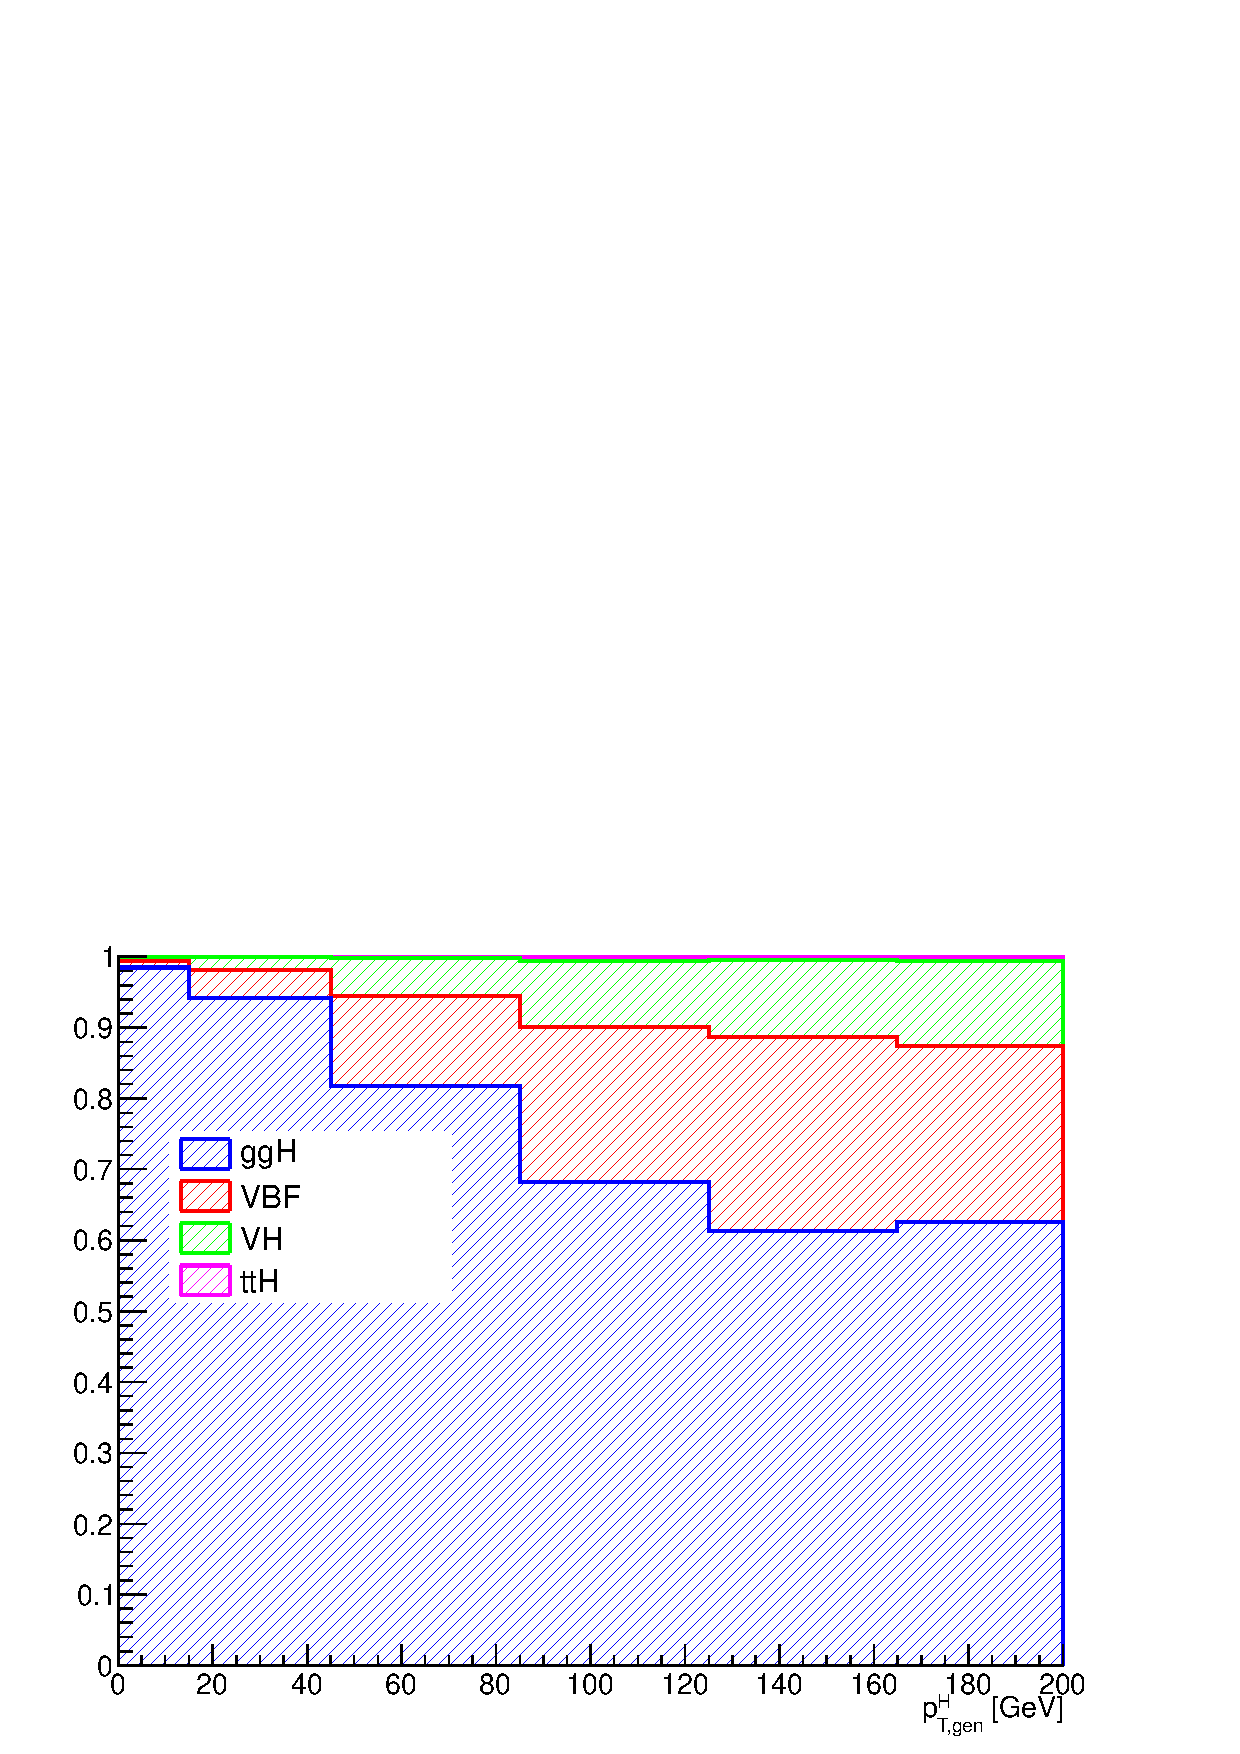
\includegraphics[width=0.7\textwidth]{images/signal_composition_ttH.pdf}
\caption{Relatve fraction of ggH, VBF, VH and ttH in each bin of the Higgs boson transverse momentum.}\label{fig:signal_comp}
\end{figure}

%\clearpage
\section{Analysis Strategy}
%%%%%%%%%%%%%%%%%%%%%%%%%%%%%%%%%%%%%%%%%%%%%%%%%%%%%%%%%%%%%%%%%%%%%%
\label{sec:AnalysisStrategy}

The analysis presented here is based on that used in the previously published \hwwllvv{}
measurements by CMS~\cite{Chatrchyan:2013iaa}, modified to be inclusive in the number of jets. 
This modification significantly reduces the uncertainties related to the modelling of the number of jets produced in association with the Higgs boson.


\subsection{Event reconstruction and selections}\label{sec:Selections}

%%% Physics objects definition
The electron selection is based on two multivariate discriminants, one specialised in identifying the electron object and the other for isolation. The cut value for each discriminant is optimised to provide a good fake electron rejection and to improve the signal acceptance.

Muons are reconstructed using the standard CMS selection and are required to be identified both in the tracker (\textit{tracker muon}) and in the muon chambers (\textit{global muon}). Additionally quality criteria on the muon track are required, such as to have at least 10 hits in the tracker (at least one of which in the pixel detector) and to have $\chi^2/ndf < 10$.
Muon isolation is based on the Particle-Flow algorithm. An MVA approach is considered, based on the radial distributions of the Particle-Flow candidates inside a cone of radius 0.5 around the muon direction.

The efficiencies for the identification and isolation of the electrons and muons are measured in data and in simulation selecting a pure sample of leptons coming from the Z$\to\ell\ell$ decay. The measured efficiencies are used as scale factors to correct the MC simulation to precisely model the data. Similarly, the trigger efficiency extracted fromdata is applied toMC samples to correct for the additional loss.

Jets in this analysis are reconstructed by combining the energy measured in the calorimeters and tracks from charged particles on basis of the standard CMS particle flow algorithm and using the anti-$k_T$ clustering algorithm with $\mathrm{R} = 0.5$. Events will be classsified into zero jet, one jet and VBF topologies by counting jets within $|\eta| < 4.7$ and for $\pt > 30$\GeV.

\textcolor{red}{Here I could add some details about jets (see AN/2012-194) if they are not already discussed in the objects section.}

Background events from \ttbar and single-top production are rejected applying a soft-muon veto and b-tagging veto. The former selection requires that in the event there are no muons from b-decays passing the following cuts: 
\begin{itemize}
\item the muon is reconstructed as TrackerMuon (and passes the TMLastStationTight ID);
\item the number of hits of the muon in the Silicon Tracker is greater than 10;
\item the transverse impact parameter of the muon is less than 0.2 cm;
\item if $\pt > 20$\GeV then the muon is required to be non-isolated with $ISO/\pt > 0.1$.

The latter veto rejects events that contain jets tagged as b-jets using two different algorithms for high and low \pt jets. For jets with \pt between 10 and 30 GeV, the Track-Counting-High-Efficiency (TCHE) algorithm, with a cut at 2.1 on the discriminating variable, is applied.
For jets above 30 GeV, a more performant algorithm, Jet-Probability (JP), is used. Jets are identified as b-jets by the JP algorithm if the discriminating variable has a value above 1.4.
In the following a b-tagged jet is defined as a jet, within $|\eta|<2.4$ (b-tagging requires the tracker information), with a value of the discriminating variable above the mentioned thresholds for the two algorithms.  


%%% Event selection
The event selection consists of several steps. The first step is to select \WW -like events applying a selection that is heavily based on the main analysis selection except for few different cuts explained below.
The \WW -like event preselection consists of the following set of cuts:
\begin{enumerate}
\item {\bf Lepton preselection}:
  \begin{itemize}
  \item at least two opposite-sign and opposite-flavour ($e\mu$) leptons reconstructed in the event;
  \item $|\eta|<2.5$ for electrons and $|\eta|<2.4$ for muons;
  \item $\pt>20~\GeV$ for the leading lepton. For the trailing lepton, the transverse momentum is required to be larger than 10~\GeV.
  \end{itemize}
\item {\bf Extra lepton veto}: the event is required to have two and only two opposite-sign leptons passing the lepton selection.
\item {\bf \MET preselection}: particle flow \MET is required to be greater than $20$\GeV.
\item {\bf Di-lepton mass cut}: $m_{\ell\ell} > 12$\GeV in order to reject low mass resonances and QCD backgrounds.
\item {\bf Di-lepton $p_T$ cut}: $p_T^{\ell\ell} > 30$\GeV.
\item {\bf projected \MET selection}: minimum projected \MET required to be larger than 20~\GeV.
\item {\bf Transverse mass}: $m_T^H>60$\GeV to reject Drell-Yan to $\tau\tau$ events. 
\end{enumerate}
In addition to the \WW-like preselection other cuts are applied in order to reduce the top background (\ttbar ans single-top), which is one of the main backgrounds in this final state. We operate two different selections depending on the number of jets with $p_T > 30$~\GeV in the event. This is done to suppress the top background both in the low $p_T^H$ region, where 0-jets events have the biggest contribution, and for higher values where also larger jet multiplicity events are important.
The selection for 0-jets events relies on a soft muon veto, which rejects events with non-isolated soft muons (likely belonging to b-jets), and on a soft jets (with $p_T < 30$~\GeV) anti b-tagging requirement.
The latter requirement exploits the Track Counting High Efficiency tagger (TCHE) to reject soft jets that are likely to come from b quarks hadronization.
These are exactly the same requirements applied in the 0-jets bin of the main analysis.

For events with a jet multiplicity greater or equal than one, we apply a different selection with respect to the main analysis. In this case we exploit the good b-tagging performances of the \textit{JetBProbability} tagger to reject all the jets with $p_T > 30$~\GeV that are likely to come from a b quark. This jet veto relies on a cut on the \textit{JetBProbability} tagger discriminant as has been also done in the VH (\hwwllnn) analysis \cite{CMS_PAS_HIG_13-017}. Any jet with a discriminant value below $1.4$ is identified as a non b-jet. The analysis selection requires no b-tagged jets with $p_T > 30$~\GeV.

\begin{figure}[b]
\centering
\includegraphics[width=0.8\textwidth]{images/cutflow2.pdf}
\caption{Effect of single selections on MC samples. The signal (red line) is multiplied by 100 and superimposed on stacked backgrounds. In each bin, corresponding to a different selection, is reported the expected number of events in MC at a luminosity of $19.46~\mathrm{fb}^{-1}$.\label{fig:cutflow}}
\end{figure}

A  cut-flow plot is reported in figure \ref{fig:cutflow} showing the effect of each selection on top of Monte Carlo samples. In the first bin, labelled as \textit{No cut}, no selection has been applied and the bin content correspond to the total expected number of events with a luminosity of $19.46~\mathrm{fb}^{-1}$. All the events in this bin have at least two leptons with a loose transverse momentum cut of $8$~\GeV. In the following bin the lepton cuts are applied, including the requirement to have two opposite-sign and opposite-flavour leptons and the extra lepton veto. Then are progressively reported all the other selections, showing the effect of each cut on backgrounds and signal. For each selection is also reported the expected signal over background ratio which after the full selection reach a maximum value around $3\%$.

\subsection{Fiducial phase space}
The Higgs boson transverse momentum is measured in a fiducial phase space, which is defined at generator level requiring
\begin{itemize}
%\item Exactly two status 3 leptons, an electron and a muon, with opposite charge, with $|\eta|<2.5$ and $\ptlmax>18~\mathrm{GeV}$ and $\ptlmin>8~\mathrm{GeV}$. No Additional status 3 lepton of any \pt
\item Exactly two status 3 leptons, an electron and a muon, originated from the \hwwllnn decays, with opposite charge, with $|\eta|<2.5$ and $\pt>20~\mathrm{GeV}$ and $\pt>10~\mathrm{GeV}$ for the leading and subleading leptons respectively.%No Additional status 3 lepton of any \pt
\item Generator level invariant mass of the two leptons $\mll>12~\mathrm{GeV}$.
%\item Vector sum of the two status 3 neutrinos $\ptvv>15~\mathrm{GeV}$.
\item Vector sum of the two status 3 leptons $\ptll>30~\mathrm{GeV}$.
\item Generator level transverse mass $\sqrt{(\ptll+\pt^{\nu\nu})^2 - (\vec{\ptll}+\vec{\pt^{\nu\nu}})^2}>50~\mathrm{GeV}$.
\end{itemize}

Experimentally, the Higgs boson transverse momentum is reconstructed as the vector sum of the lepton momenta in the transverse plane and \MET.
\begin{equation}
\vec{p}_\mathrm{T}^\mathrm{\,H} = \vec{p}_\mathrm{T}^{\,\ell\ell} + \vec{p}_\mathrm{T}^\mathrm{\,miss}
\end{equation}
Compared to other differential analysis of the Higgs cross section, such as those in the ZZ and $\gamma\gamma$ decay channels, this analysis has to cope with the limited resolution due to the \MET entering the transverse momentum measurement.
The effect of the limited \MET resolution has two main implications on the analysis strategy:
\begin{itemize}
\item the choice of the binning in the transverse momentum spectrum needs to be reasonable when compared to the resolution. A detailed explanation of how the binning is defined is given in Sec.~\ref{sec:Binning}.
\item Non negligible bin migration effects are present, and an unfolding procedure needs to be applied, not only to correct for selection efficiencies, as in ZZ and $\gamma\gamma$, but also to correct for bin migration effects. This is explained in Sec.~\ref{sec:Unfolding}.
\end{itemize}

A detailed description of the fiducial region definition and about its optimization is given in appendix \ref{app:fiducial_region}.


\subsection{Binning of the \pth distribution}

\textcolor{red}{Put here also the plots with efficiency and fakes in each \pth bin}.











%\clearpage
%\input{Chapter4/Selections.tex}
%\clearpage
%\input{Chapter4/Binning.tex}
%\clearpage
\section{Background estimation}
%%%%%%%%%%%%%%%%%%%%%%%%%%%%%%%%%%%%%%%%%%%%%%%%%%%%%%%%%%%%%%%%%%%%%%
\label{sec:Backgrounds}

\textcolor{red}{Add plots for each background process}

\subsection{Top quark background \label{sec:TTBackground}}

In this analysis the top quark background is divided into two different categories depending on the number of jets in the event. In the two categories different selections are applied, especially concerning the b-tagging requirements.

The general strategy for determining the residual top events in the signal region is to first measure the top tagging efficiencies from an orthogonal region of phase space in data. The orthogonal phase space is  defined inverting the b-veto requirement of the signal region, in such a way to have a control region enriched in top quark events.  Then, using this efficiency, the number of events with the associated uncertainty is propagated from the control region to the signal region.
The number of surviving top events in the signal region would then be:

\begin{equation}
 N^{\mathrm{signal}}_{bveto} = N^{\mathrm{control}}_{btag} \cdot \frac{1-\epsilon_{\mathrm{top}}}{\epsilon_{\mathrm{top}}}
\label{eq:top_equation}
\end{equation}

where $N^{\rm control}_{\rm btag}$ is the number of events in the 
control region and $\epsilon_{\rm top}$ is the efficiency as measured
in data.

The methods to estimate the top background contribution in the two jet categories are different and are explained below.


\subsubsection{0-jets category}
Most of the top background, composed of \ttbar and tW processes, is rejected in the 0-jet bin by the
jet veto. The top-tagging efficiency in the zero jet bin, $\epsilon_{\rm tag}^{0-jet}$, is the probability for a top event to
fail one of either the b-tagging veto or the soft muon veto, and is defined as:

\begin{equation}\label{eq:eff_top_0j}
\epsilon_{\rm tag} = \frac{N_{\rm tag}^{\rm control}}{N^{\rm control}} \quad ,
\end{equation}

where $N^{\rm control}$ is the number of events in the top control phase space defined requiring one b-tagged jet with $\pt>30$\GeV, and $N_{\rm tag}^{\rm control}$ is the subset of those events that pass either the soft muon tagging or the low-\pt b jet tagging. The purity of this control sample, as estimated from simulation, is about 97\%. The remaining 3\% background contribution is estimated from simulation and subtracted from the numerator and denominator of Eq.~\eqref{eq:eff_top_0j}. The efficiency $\epsilon_{\rm top}^{0-jet}$ can then be estimated using the following formula:

\begin{equation}\label{eq:eff_top_0j}
\epsilon_{\rm top}^{0-jet} = f_{\ttbar} \cdot \epsilon_{2b} + f_{tW} \cdot ( x \cdot \epsilon_{2b} + (1-x) \cdot \epsilon_{\rm tag} ) \quad ,
\end{equation}

\begin{equation}
\epsilon_{2b} = 1 - (1 - \epsilon_{\rm tag})^{2} \quad ,
\end{equation}
where $f_{\ttbar}$ and $f_{tW}$ are the \ttbar and tW fractions respectively, $x$ is the fraction of tW events containing 2 b jets, and $\epsilon_{2b}$ is the efficiency for a top event with 0 counted jets, i.e. two soft b jets, to pass the top veto. For the ratio of \ttbar and tW cross-sections an uncertainty of 17\% is assumed. The fraction $f_{\ttbar}$ is estimated using MC simulation of the \ttbar and tW processes at NLO accuracy.

Using this procedure a data/simulation scale factor of $0.98 \pm 0.17$ is found, and is applied to correct the MC simulation in order to match the data.



\subsubsection{Category with more than 0 jets}
The strategy for the estimation of the top background in events with at least one jet with $\pt$ greater than 30 \GeV is the following. First of all the efficiency for tagging a b jet is measured both in data and simulation and the values are used to correct the simulation for different b-tagging efficiencies in data and simulation. This evaluation is performed in a control region, called CtrlTP, containing at least two jets, using a Tag\&Probe technique. The procedure to extract these scale factors is presented in Sec.~\ref{sec:TagAndProbe}. Then a larger statistics control region, CtrlDD, is defined by requiring at least one b-tagged jet and we use the simulation, corrected for the previously computed b-tagging efficiency scale factor, to derive the factor that connects the number of events in CtrlDD to the number of events in the signal region. This second step is explained in detail in Sec.~\ref{sec:DD}. 

\subsubsection{Tag\&Probe \label{sec:TagAndProbe}}
The Tag\&Probe technique is a method to estimate the efficiency of a selection on data. In can be applied whenever one has two objects in one event, by using one of the two, the \tg{}, to identify the process of interest, and using the second, the \probe{}, to actually measure the efficiency of the selection being studied. In our case we want to measure the b-tagging efficiency, so what we need is a sample with two b-jets per event. The easiest way to construct such a sample is to select $t\bar{t}$ events.

The CrtlTP control region is defined selecting the events which pass the lepton preselection cuts listed in Sec.~\ref{subsec:EventSelection}, and have at least two jets with \pt greater than 30 \GeV.
One of the two leading jets is required to have a \jpb score higher than 0.5. From events in this control region we built \tp{} pairs as follows. For each event the two leading jets are considered. If the leading jet passes the \jpb cut of 0.5, that is considered a \tg{}, and the sub-leading jet is the \probe{}. In order to avoid any bias that could arise from the probe being always the second jet, the pair is tested also in reverse order, meaning that the sub-leading jet is tested against the \tg{} selection, and in case it passes, then the leading jet is used as \probe{} in an independent \tp{} pair. This means that from each event passing the CrtlTP cuts one can build up to two \tp{} pairs. 

If the \tg{} selection were sufficient to suppress any non top events, one could estimate the efficiency by dividing the number of \tp{} pairs in which the \probe{} passes the analysis cut \jpb$>$1.4 (\tpp) by the total number of \tp{} pairs. However this is not the case. 
In order to estimate the efficiency in the presence of background a variable that discriminates between true b-jets and other jets in a $t\bar{t}$ sample is chosen. The variable is the \pt of the \probe{} jet. For real b-jets this variable has a peak around 60 \GeV, while it does not peak for other jets. The idea is to fit simultaneously the \pt spectrum for \probe{} jets in \tpp{} and \tfp{} pairs, linking together the normalizations of the two samples as follows:
\begin{equation}
N_{TPP}=N_{s}\epsilon_{s} + N_b\epsilon_{b}
\end{equation}
\begin{equation}
N_{TFP}=N_{s}(1-\epsilon_{s}) + N_b(1-\epsilon_{b})
\end{equation}
where $N_{\rm TPP}$ is the number of \tpp{} pairs, $N_{\rm TFP}$ is the number of \tfp{} pairs, $N_{\rm s}$ is the number of \tp{} pairs in which the probe is a b-jet, $N_{\rm b}$ is the number of \tp{} pairs in which the probe is a not b-jet, $\epsilon_{\rm s}$ is the b-tagging efficiency, $\epsilon_{\rm b}$ is the probability of identifying as b-jet a non-b-jets, i.e. the mistag rate. 

A $\chi^{2}$ simultaneous fit of the \probe{} \pt spectrum for \tpp{} and \tfp{} pairs is performed, deriving the shapes for true b-jets and non-b-jets from the simulation, and extracting $N_{\rm s}$, $N_{\rm b}$, $\epsilon_{\rm s}$ and $\epsilon_{\rm b}$ from the fit.
The result of the fit on simulation is shown in Fig.~\ref{fig:mc_tp}. The relevant efficiencies are:
\begin{equation}
\epsilon_{s}^{MC}=0.7663\pm0.0072
\end{equation}
\begin{equation}
\epsilon_{b}^{MC}=0.208\pm0.015
\end{equation}
We have checked that these values are consistent with the true value for the b-tagging efficiency. The true value is computed by selecting jets that are matched within a cone of $\Delta{R}<0.5$ with a generator level b-quark, and counting the faction of those that pass the \jpb cut of 1.4. This means that the \tp{} method does not introduce biases within the simulation statistic accuracy.

\begin{figure}[b]
\centering
\includegraphics[width=0.8\textwidth]{images/mc_pt_probe.pdf}
\caption{Simultaneous fit of the \tpp{} and \tfp{} pairs in the MC.\label{fig:mc_tp}}
\end{figure}

In order to assess the robustness of the fit, 5000 toy MC samples have been generated with a statistics equivalent to the one expected in data and the same fit is performed. All the 5000 fit succeeded, and the pull distributions for $\epsilon_{\rm s}$ and $\epsilon_{\rm b}$ parameters are shown in Fig.~\ref{fig:pullstp}. The plots show the pull of the efficiencies measured in the fit, where the pull variable for each toy $i$ is defined as:

\begin{equation}
pull(\epsilon_{\rm s (b)}) = \frac{\epsilon_{\rm s (b)}^{\rm true} - \epsilon_{\rm s (b)}^{i}}{\sigma(\epsilon_{\rm s (b)}^{i})}
\end{equation}

The pulls are centered on 0 and have $\sigma$ close to 1, as expected.

\begin{figure}[t]
\centering
\includegraphics[width=0.8\textwidth]{images/pulls_mc.pdf}
\caption{Pulls of the $\epsilon_{s}$ and $\epsilon_{b}$ parameters in 5000 toy MC.\label{fig:pullstp}}
\end{figure}
An example fit for one of the toys is shown in  Fig.~\ref{fig:toy_tp}
\begin{figure}[b]
\centering
\includegraphics[width=0.8\textwidth]{images/mc_pt_probe_toy.pdf}
\caption{Fit of a toy MC sample.\label{fig:toy_tp}}
\end{figure}

Before running the fit on data we have tried to validate the shapes used in the fit with data. To do so, we have made a much more pure $t\bar{t}$ selection, by requiring exactly two jets with \jpb score higher than 1.5 and no additional b-tagged jets, even if they have $\pt$ smaller than 30 \GeV. On this purer sample we have compared data against the shape used to fit the true b-jets in the \tpp{} distribution. The result is shown in Fig.~\ref{fig:purett} and shows good agreement.
\begin{figure}[t]
\centering
\includegraphics[width=0.6\textwidth]{images/passprobe_data_mc.pdf}
\caption{Shape comparison for the \probe{} $\pt$ spectrum in data and in MC in a very pure $t\bar{t}$ sample.\label{fig:purett}}
\end{figure}

We have finally performed the fit on data, as shown in Fig.~\ref{fig:data_tp}, which results in in the following efficiencies:
\begin{equation}
\epsilon_{s}^{Data}=0.769\pm0.022
\end{equation}
\begin{equation}
\epsilon_{b}^{Data}=0.121\pm0.054
\end{equation}

\begin{figure}[b]
\centering
\includegraphics[width=0.8\textwidth]{images/data_ptprobe.pdf}
\caption{Simultaneous fit of the \tpp{} and \tfp{} pairs in data.\label{fig:data_tp}}
\end{figure}
Further checks on the Tag\&Probe efficiencies are shown in Appendix~\ref{app:tpfractw}, which concern the uncertainty related to the not perfect knowledge of the $tW/t\bar{t}$ ratio in the MC.


\subsubsection{Data driven estimation \label{sec:DD}}
In addition to the b-tagging efficiency, the other ingredient to estimate the $t\bar{t}$ background is the process cross section. The idea is to measure the cross section in a $t\bar{t}$ enriched control region, that we call CtrlDD. CtrlDD is defined according to the lepton preselection cuts defined in Sec.~\ref{subsec:EventSelection}, and requiring in addition at least one jet with \jpb score higher than 1.4.

From the simulation we derive the factor $\alpha$ that connects CrtlDD to the signal region, from the ratio of $t\bar{t}$ events in the two regions.
\begin{equation}
\alpha=\frac{N_{t\bar{t}~MC}^{SIG}}{N_{t\bar{t}~MC}^{CtrlDD}}.
\end{equation}
We then count events CtrlDD in data, we subtract the expected number of events from non-$t\bar{t}$ backgrounds, and we obtain $N_{t\bar{t}~Data}^{CtrlDD}$. We finally obtain the number of expected $t\bar{t}$ events in the signal region ($N_{t\bar{t}~Data}^{SIG}$) as:
\begin{equation}
N_{t\bar{t}~Data}^{SIG} = \alpha{}N_{t\bar{t}~Data}^{CtrlDD}.
\end{equation}

In evaluating $\alpha$ and its error we made use of the b-tagging efficiencies determined in Sec.~\ref{sec:TagAndProbe}. 
%Since the efficiency and mistag rate that we have measured on data are close to the one in the MC we have decided assume a scale factor of 1 for both b-tagging efficiency and mis-tag rate, with an error that covers all of the difference between data and MC and the statistical uncertainty of the Tag\&Probe fit. In other other 
For each event we derive an efficiency scale factor and a mistag rate scale factor, depending on whether the event is in the signal or CtrlDD regions.
\begin{equation}
\label{eq:sfsig}
SF_{SIG} = \left(\frac{1-\epsilon_{s}^{Data}}{1-\epsilon_{s}^{MC}}\right)^{min(2, n_{b-jets})} \left(\frac{1-\epsilon_{b}^{Data}}{1-\epsilon_{b}^{MC}}\right)^{n_{non-b-jets}} 
\end{equation}

\begin{equation}
\label{eq:sfbkg}
SF_{CtrlDD} = \left(\frac{\epsilon_{s}^{Data}}{\epsilon_{s}^{MC}}\right)^{(jet1 == b-jet)} \left(\frac{\epsilon_{b}^{Data}}{\epsilon_{b}^{MC}}\right)^{(jet1 == non-b-jets)} 
\end{equation}
where $n_{b-jets})$ is the number of true b-jets in the event and $n_{non-b-jets}$ is the number of non-b-jets in the event. The writing $jet1 == b-jet$ ($jet1 == non-b-jets$) is a boolean flag that is true when the leading jet, the one used for the CtrlDD selection, is (not) a true b-jet.

Since the efficiency and mistag rate that we have measured on data are close to the one in the MC we have decided to assume a scale factor of 1 for both b-tagging efficiency and mis-tag rate. This means that the central values of the scale factors defined in Eq.~\ref{eq:sfsig} and Eq.~\ref{eq:sfbkg} is 1, but these numbers have an error that is derived assuming an uncertainty on $\epsilon_{s}^{Data}$ and $\epsilon_{b}^{Data}$ that covers both the statistical error from the fit of the two quantities and the difference with respect to the MC.
This results in an up variation and a down variation of the scale factors in the signal region and CtrlDD regions, that is used to derive an error on $\alpha$.

We have decided to make a data driven estimation of the $t\bar{t}$ background with the method described above in each of the $\pth$ bins independently. The reason why we have chosen to make this estimation in $\pth$ bins, rather than inclusively is explained in Fig.~\ref{fig:ttpth}. In this plot the $t\bar{t}$ background is normalized to the cross section measured by CMS. The binning is the same chosen for the analysis. As shown in the ratio plot, an overall normalization factor would not be able to accommodate for the variations of the Data/MC ratio from bin to bin.
\begin{figure}[b]
\centering
\includegraphics[width=0.6\textwidth]{images/ttpth.pdf}
\caption{$\pth$ variable in the CtrlDD control region.\label{fig:ttpth}}
\end{figure}

The $\alpha$ factors for each bin and the number of events in signal, CtrlDD region in MC as well as in data are listed in Tab.~\ref{tab:ttdd}.
%\centering
%\begin{tabular}{c c c c c c}
%\hline
%$\pth$ bin & $N_{t\bar{t}~Data}^{CtrlDD}$ & $N_{t\bar{t}~MC}^{CtrlDD}$ & $N_{t\bar{t}~MC}^{SIG}$ & $\alpha$ & $\Delta\alpha$ \\
%\hline
%1 & 406.73 & 358.78 & 117.83 & 0.328 & 0.075 \\ 

%2 & 2929.25 & 2703.44 & 859.08 & 0.318 & 0.071 \\ 

%3 & 5723.95 & 5465.37 & 1567.86 & 0.287 & 0.065 \\ 

%4 & 3863.39 & 3774.66 & 799.41 & 0.212 & 0.052 \\ 

%5 & 1533.61 & 1589.53 & 292.06 & 0.184 & 0.055 \\ 

%6 & 703.52 & 825.11 & 214.33 & 0.256 & 0.140 \\ 
%\hline

\begin{table}
\centering
\begin{tabular}{c c c c c c}

\hline\hline

$p_T^H$ bin & $N_{CTRL}^{DATA}$ & $N_{CTRL}^{TOP}$ &  $N_{SIG}^{TOP}$ &
$\alpha$ & $\Delta\alpha$ \\ 

\hline

1 & 406.71 & 358.78 & 117.83 & 0.328 & 0.075 \\ 

2 & 2930.14 & 2703.44 & 859.08 & 0.318 & 0.071 \\ 

3 & 5481.02 & 5207.48 & 1506.05 & 0.289 & 0.065 \\ 

4 & 4126.35 & 4032.56 & 861.22 & 0.214 & 0.052 \\ 

5 & 1612.64 & 1654.27 & 304.69 & 0.184 & 0.055 \\ 

6 & 647.50 & 760.37 & 201.70 & 0.265 & 0.147 \\ 

\hline

\end{tabular}
\caption{Table of data driven scale factors.\label{tab:ttdd}}
\end{table}
A comparison of the $\mll$ distribution in the six $\pth$ bins used in the analysis in CtrlDD after the data driven correction is shown in Fig.~\ref{fig:mllCtrlDD}
\begin{figure}[htb]
\centering
\subfigure[$\pth<15\GeV$]{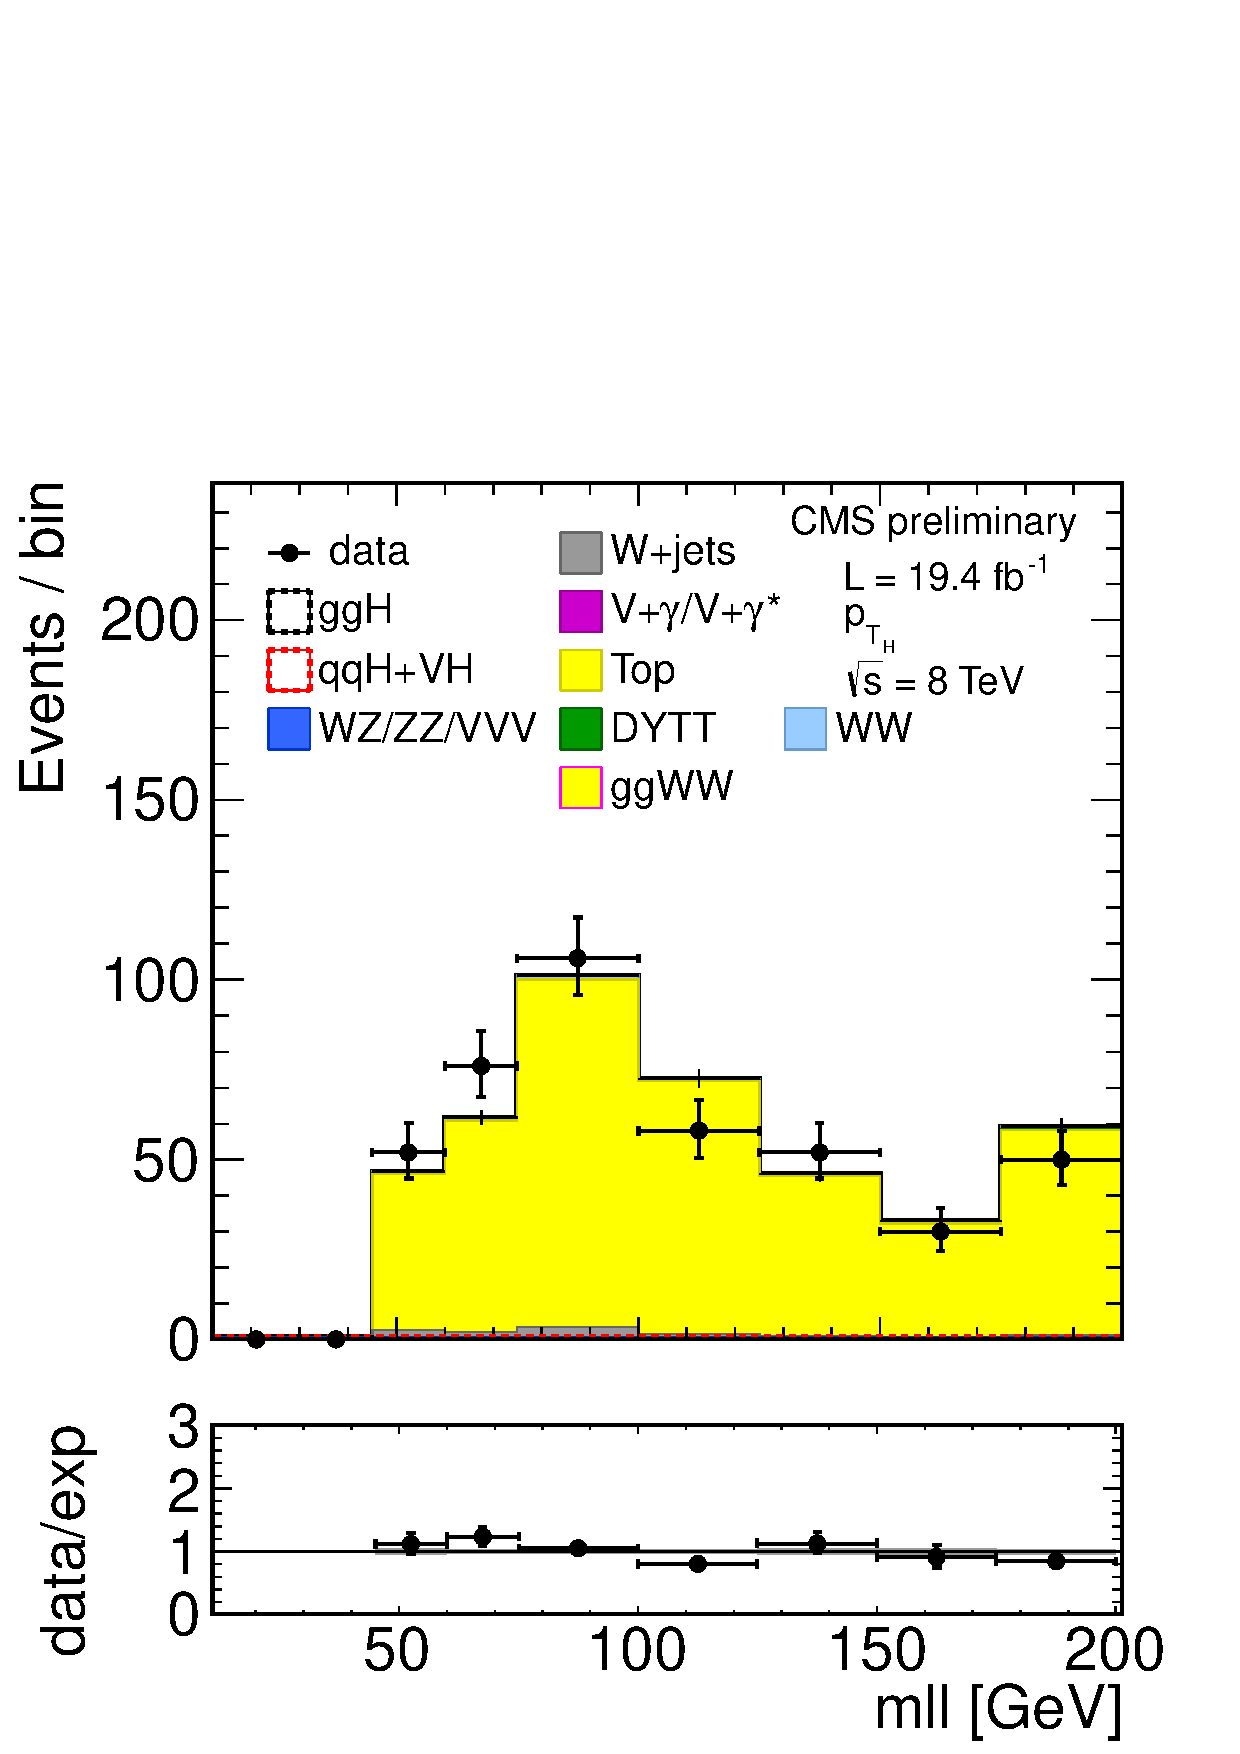
\includegraphics[width=0.35\textwidth]{images/mllBin0CtrlDD.pdf}}
\subfigure[$15\GeV<\pth<45\GeV$]{\includegraphics[width=0.35\textwidth]{images/mllBin1CtrlDD.pdf}}

\subfigure[$45\GeV<\pth<85\GeV$]{\includegraphics[width=0.35\textwidth]{images/mllBin2CtrlDD.pdf}}
\subfigure[$85\GeV<\pth<125\GeV$]{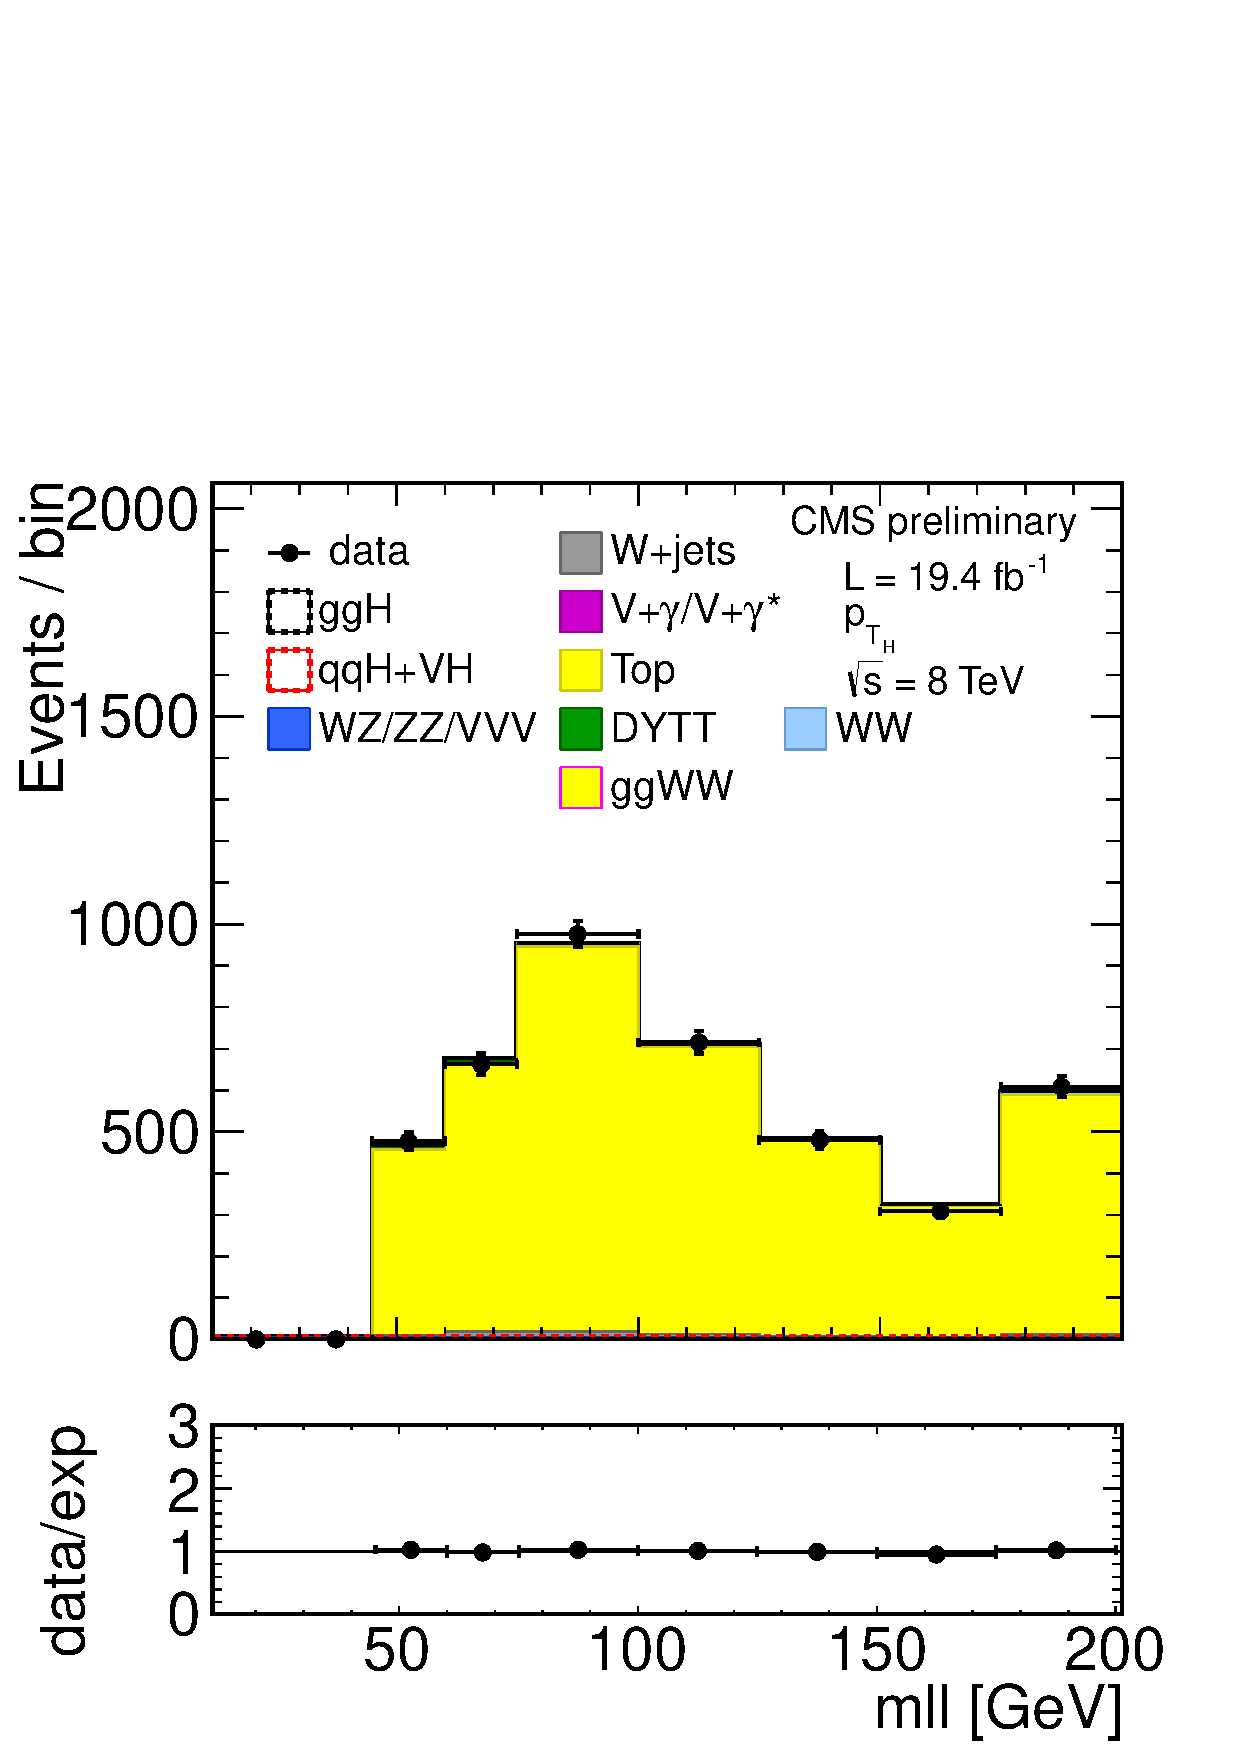
\includegraphics[width=0.35\textwidth]{images/mllBin3CtrlDD.pdf}}

\subfigure[$125\GeV<\pth<165\GeV$]{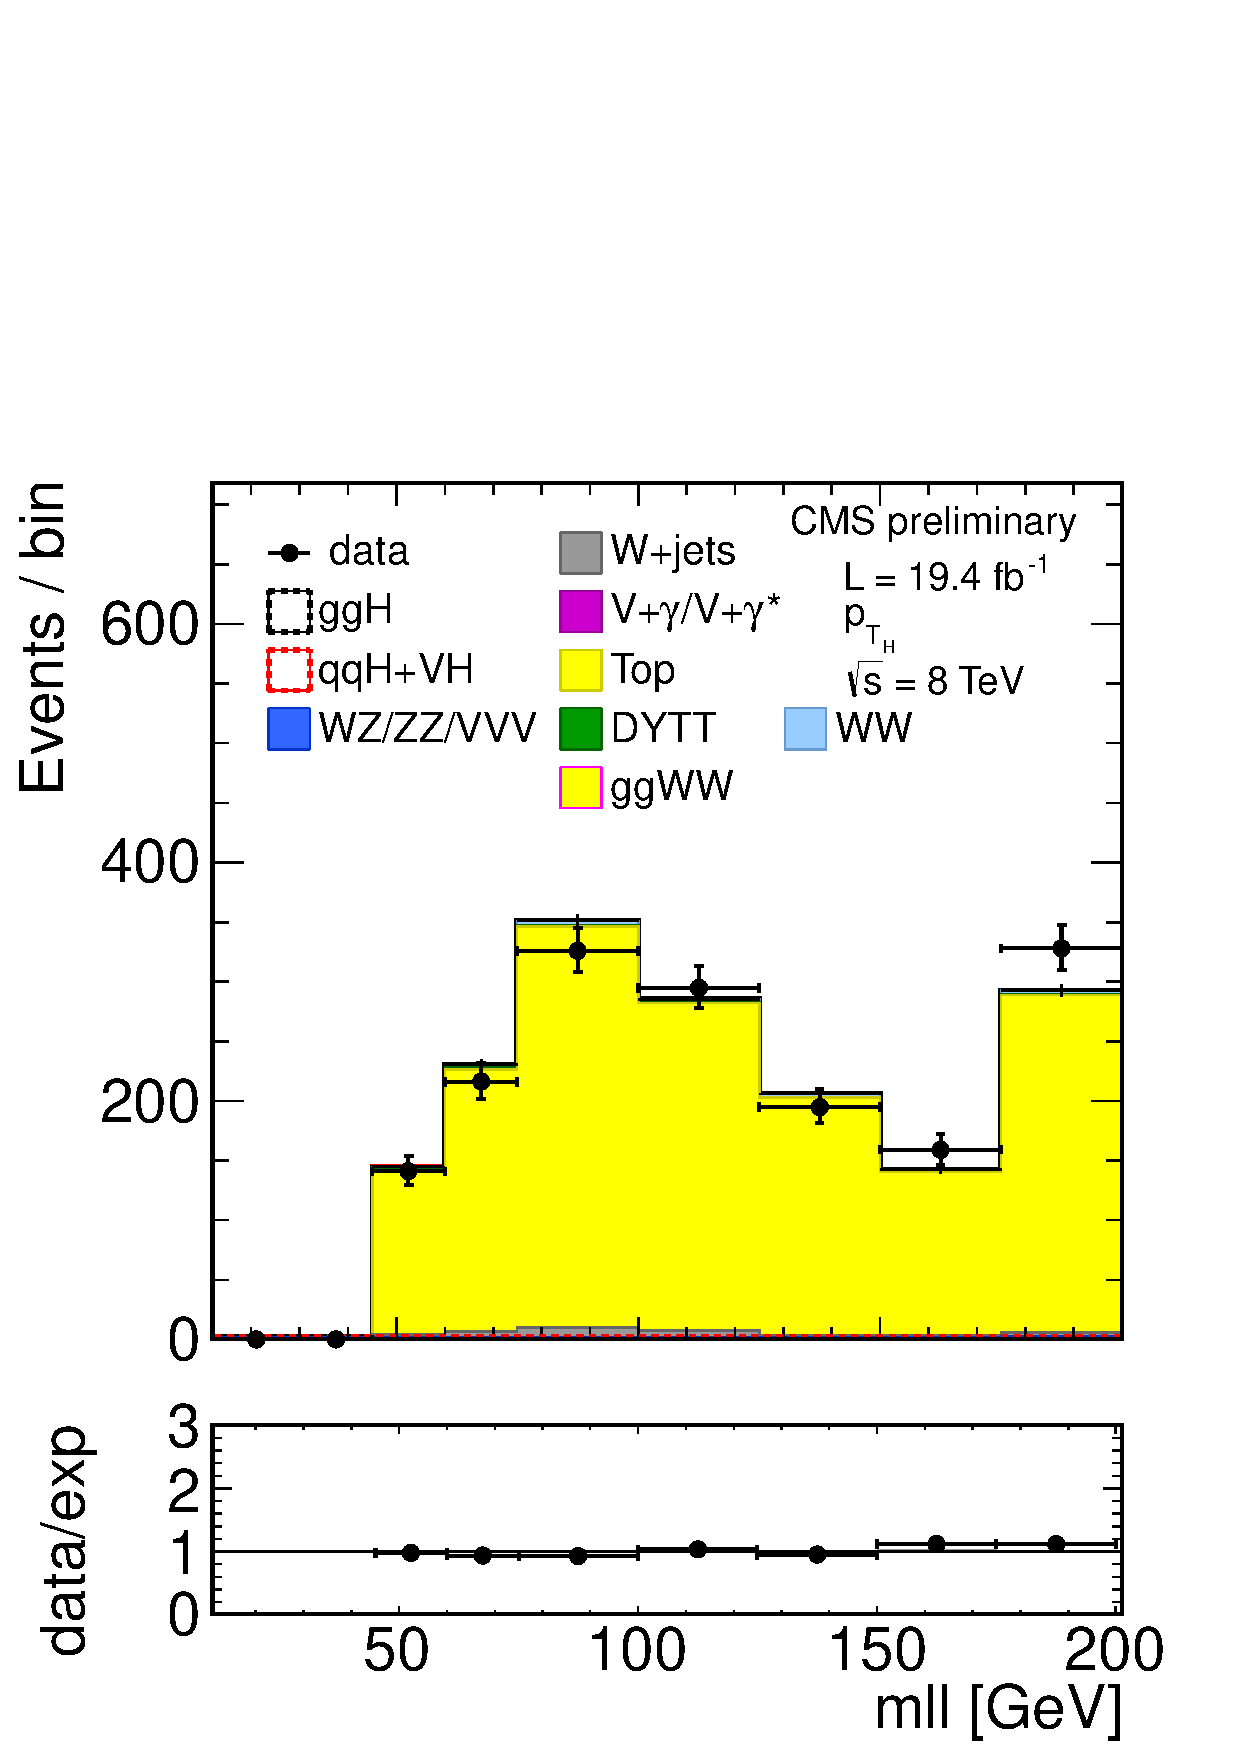
\includegraphics[width=0.35\textwidth]{images/mllBin4CtrlDD.pdf}}
\subfigure[$\pth>165\GeV$]{\includegraphics[width=0.35\textwidth]{images/mllBin5CtrlDD.pdf}}
\caption{$\mll$ distributions in the CtrlDD region for the different $\pth$ bins.\label{fig:mllCtrlDD}}
\end{figure}

























\clearpage
\subsection{\WW background \label{sec:WWBackground}}

For what the WW background shape is concerned the prediction from the Monte-Carlo simulation has been used.
This background is divided into six different parts, corresponding to the six bins of \pth considered. In each bin the normalization of the WW background is left free to float and is thus adjusted to match the data by the fit. In this way we minimize an effect that has been observed also in \cite{CMS_AN_2014_056}, that is a difference in shape between the $p_\mathrm{T}^\mathrm{WW}$ theory prediction and the distribution provided by the MC simulation, in our case by \textsc{Madgraph}.\\
In figure \ref{fig:ww_wwnlo} a comparison is shown between the $p_\mathrm{T}^\mathrm{WW}$ spectra of two different qqWW samples: the blue line corresponds to the WW \textsc{Madgraph} samples that we use in this analysis and the red line refers to the same sample in which a reweighting has been applied in order to match the theoretical prediction at NLO+NNLL precision. 
\begin{figure}[b]
\centering
\includegraphics[width=0.7\textwidth]{images/WWnlo/WW_WWnlo.pdf}
\caption{}\label{fig:ww_wwnlo}
\end{figure}
A shape discrepancy can be clearly observed and the effect becomes larger at high values of \pth.\\
In order to assess if these discrepancy has a not negligible effect on the shapes of the variables that we use for the fit, \mll and \mt, we checked these distributions in every \pth bin, comparing several samples. In particular we compared the \textsc{Madgraph} sample used for the nominal shape, the \textsc{Madgraph} sample with NLO+NNLL  reweighting, a \textsc{Powheg} NLO sample and an \textsc{aMC@NLO} sample.
The results of this comparison are shown in figures \ref{fig:ww_mll} and \ref{fig:ww_mth}. The discrepancy in shape among the different models is within the statistical accuracy of the MC samples. 

\begin{figure}[htb]
\centering
\subfigure[\mll bin 1]{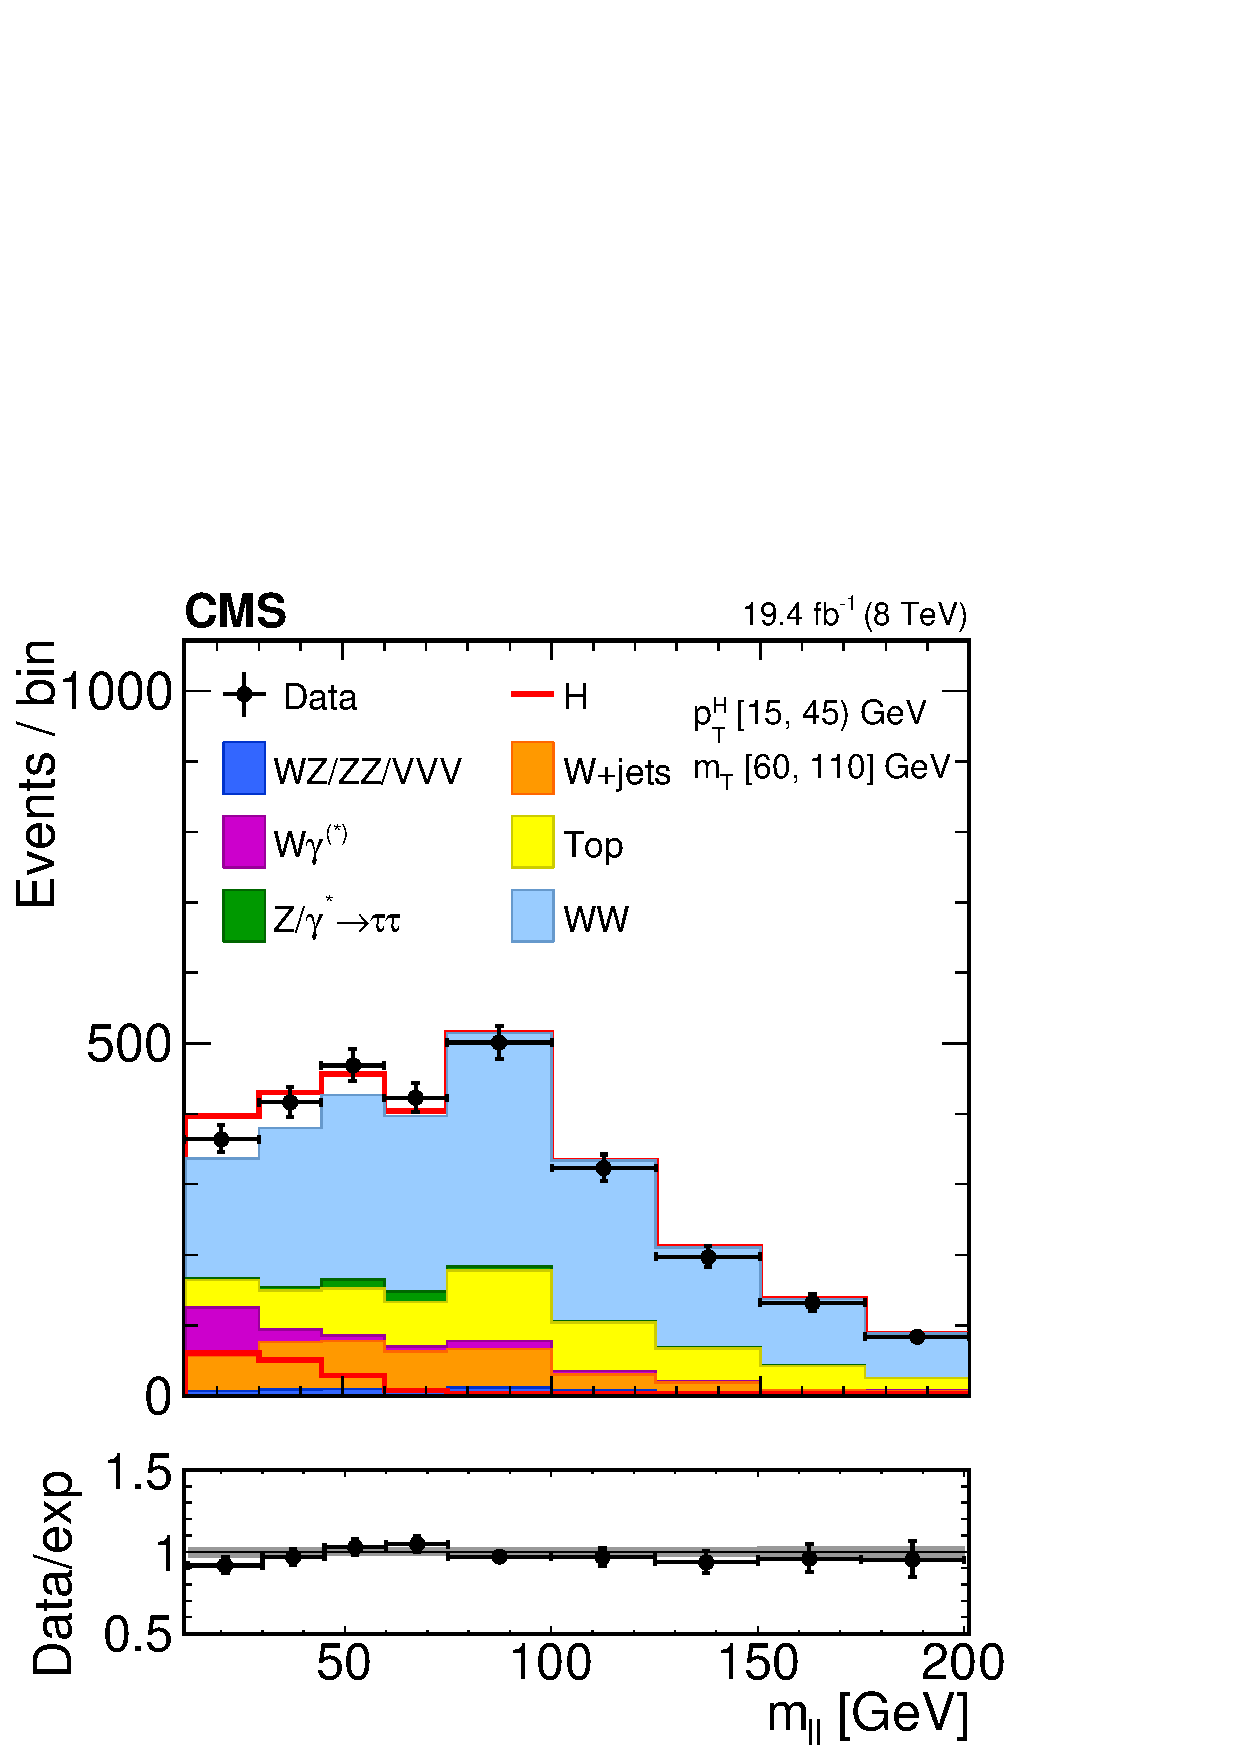
\includegraphics[width=0.45\textwidth]{images/WWnlo/mllBin1.pdf}}
\subfigure[\mll bin 2]{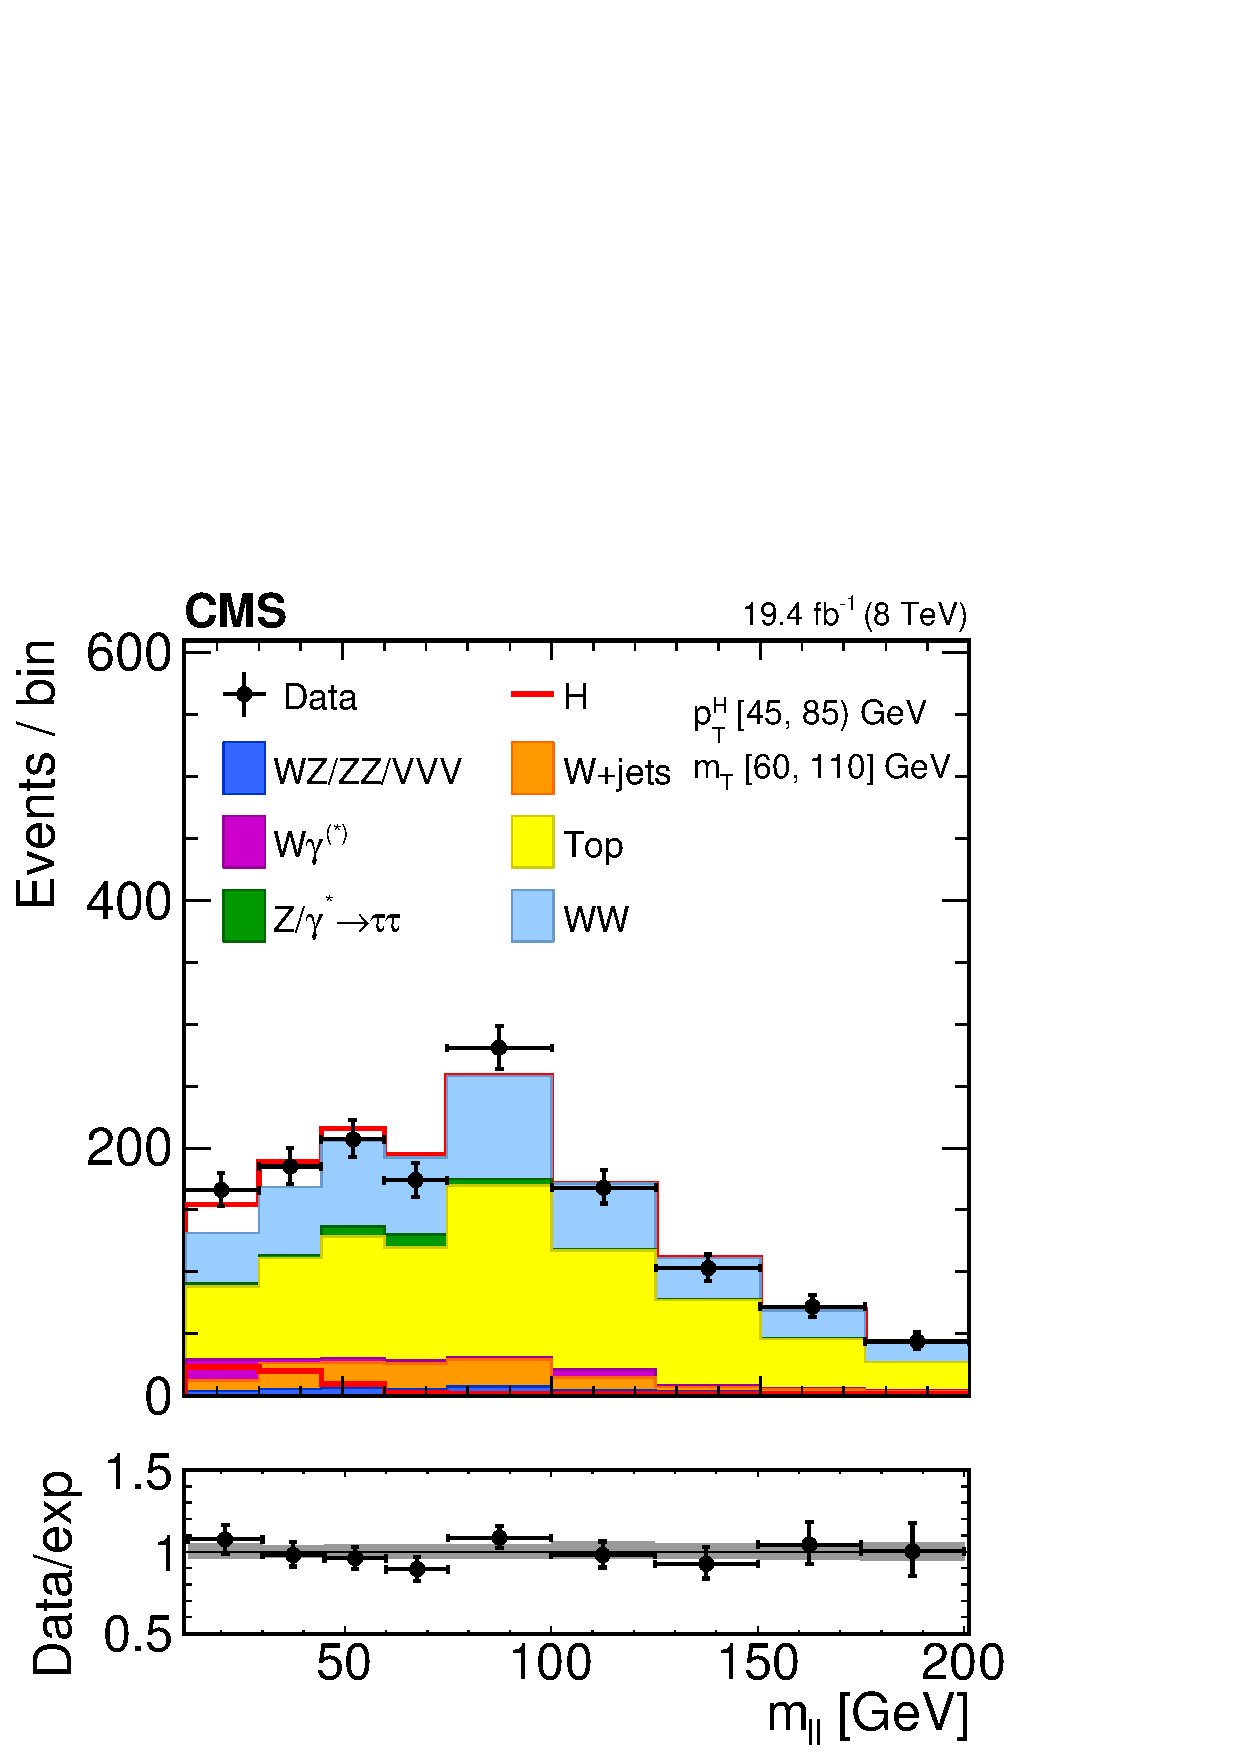
\includegraphics[width=0.45\textwidth]{images/WWnlo/mllBin2.pdf}}\\
\subfigure[\mll bin 3]{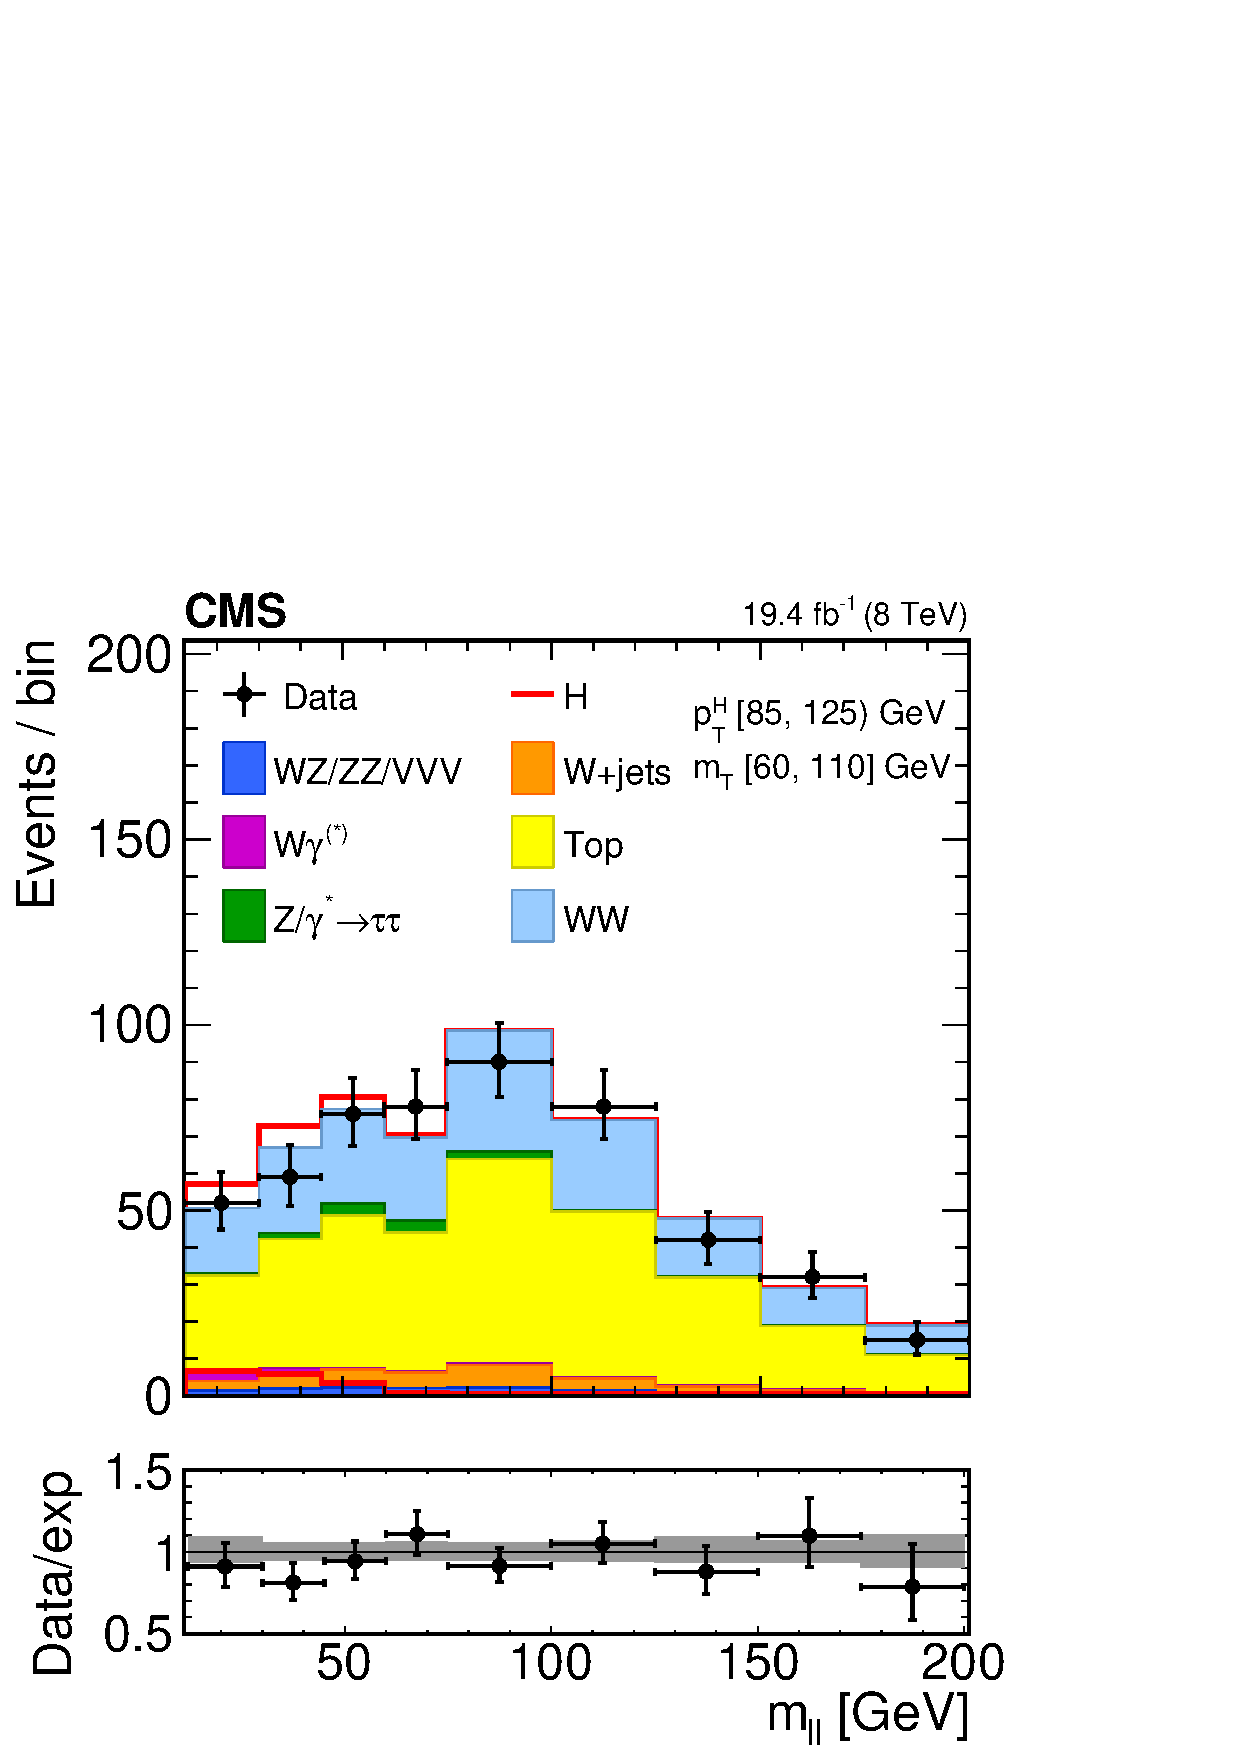
\includegraphics[width=0.45\textwidth]{images/WWnlo/mllBin3.pdf}}
\subfigure[\mll bin 4]{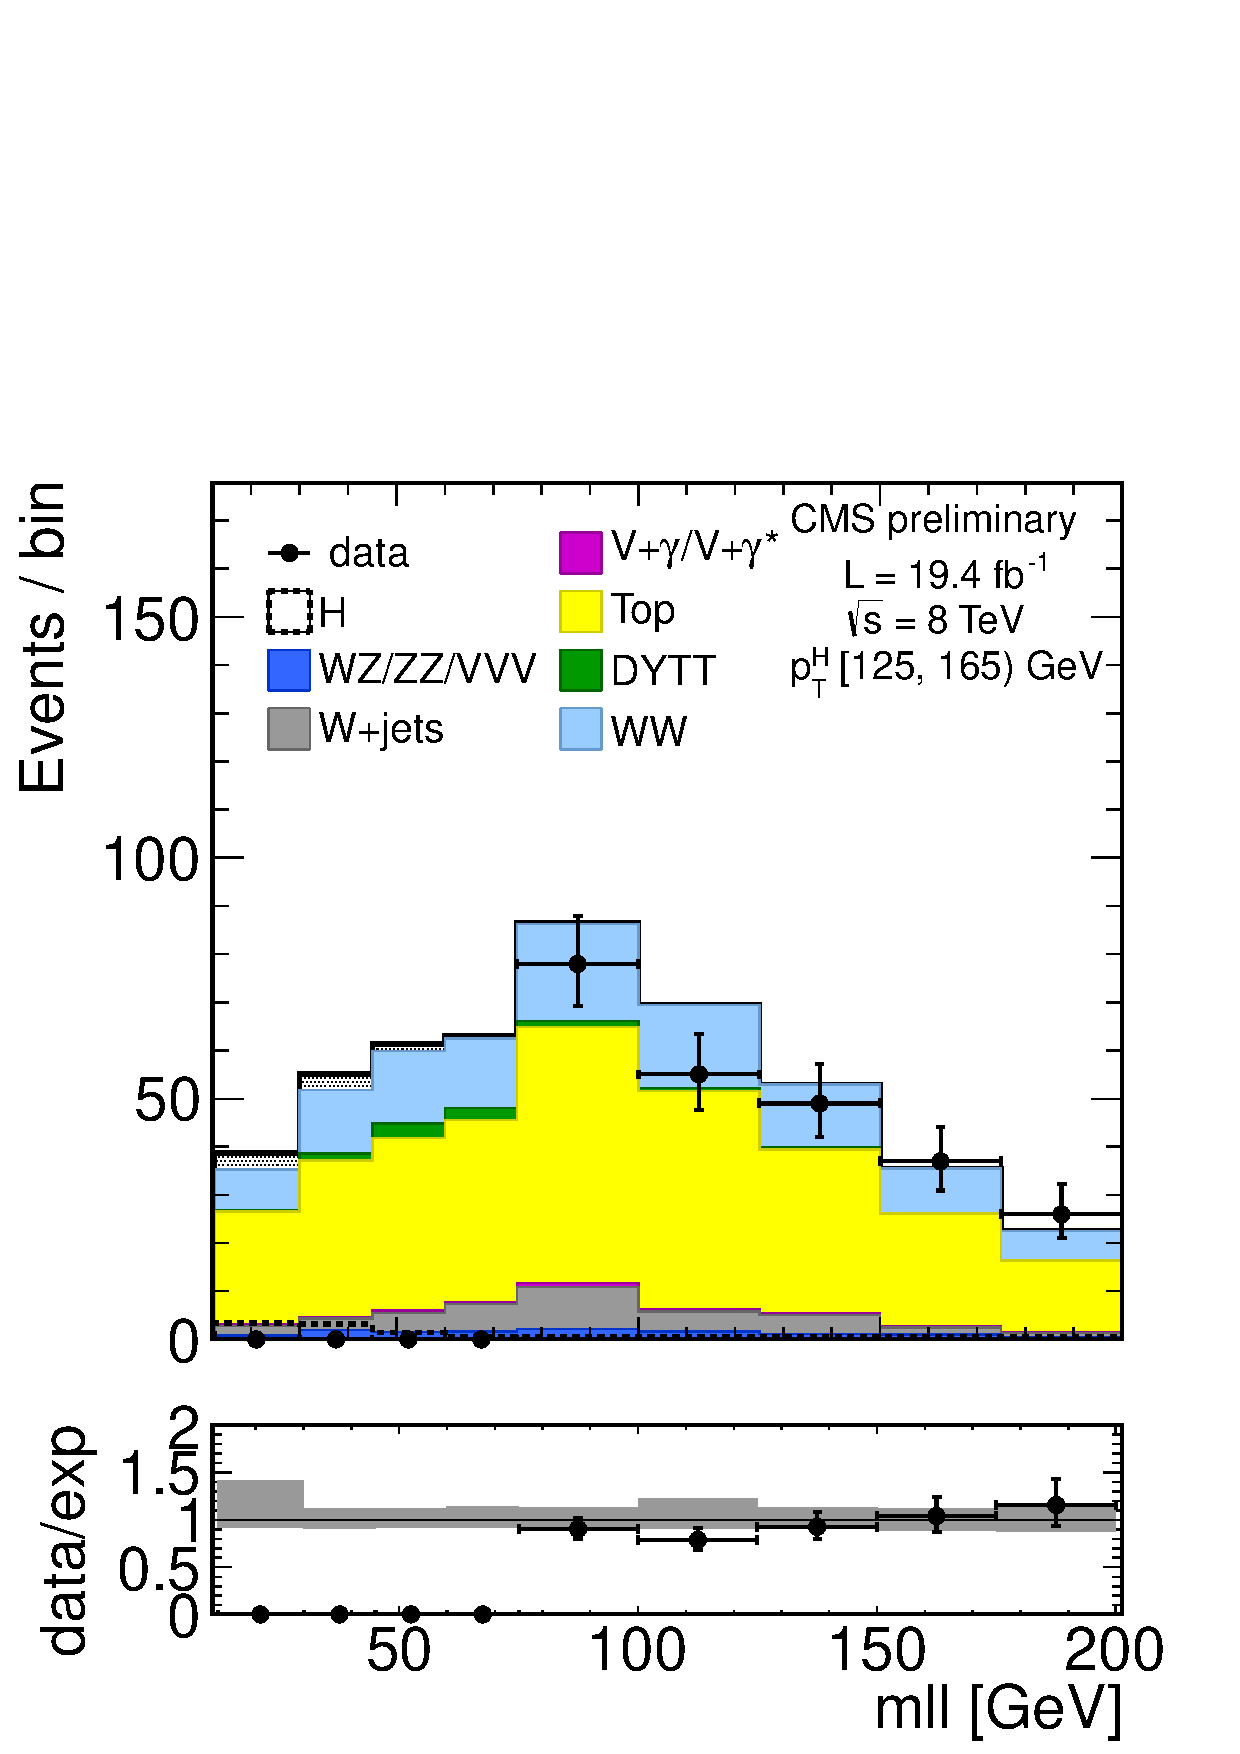
\includegraphics[width=0.45\textwidth]{images/WWnlo/mllBin4.pdf}}\\
\subfigure[\mll bin 5]{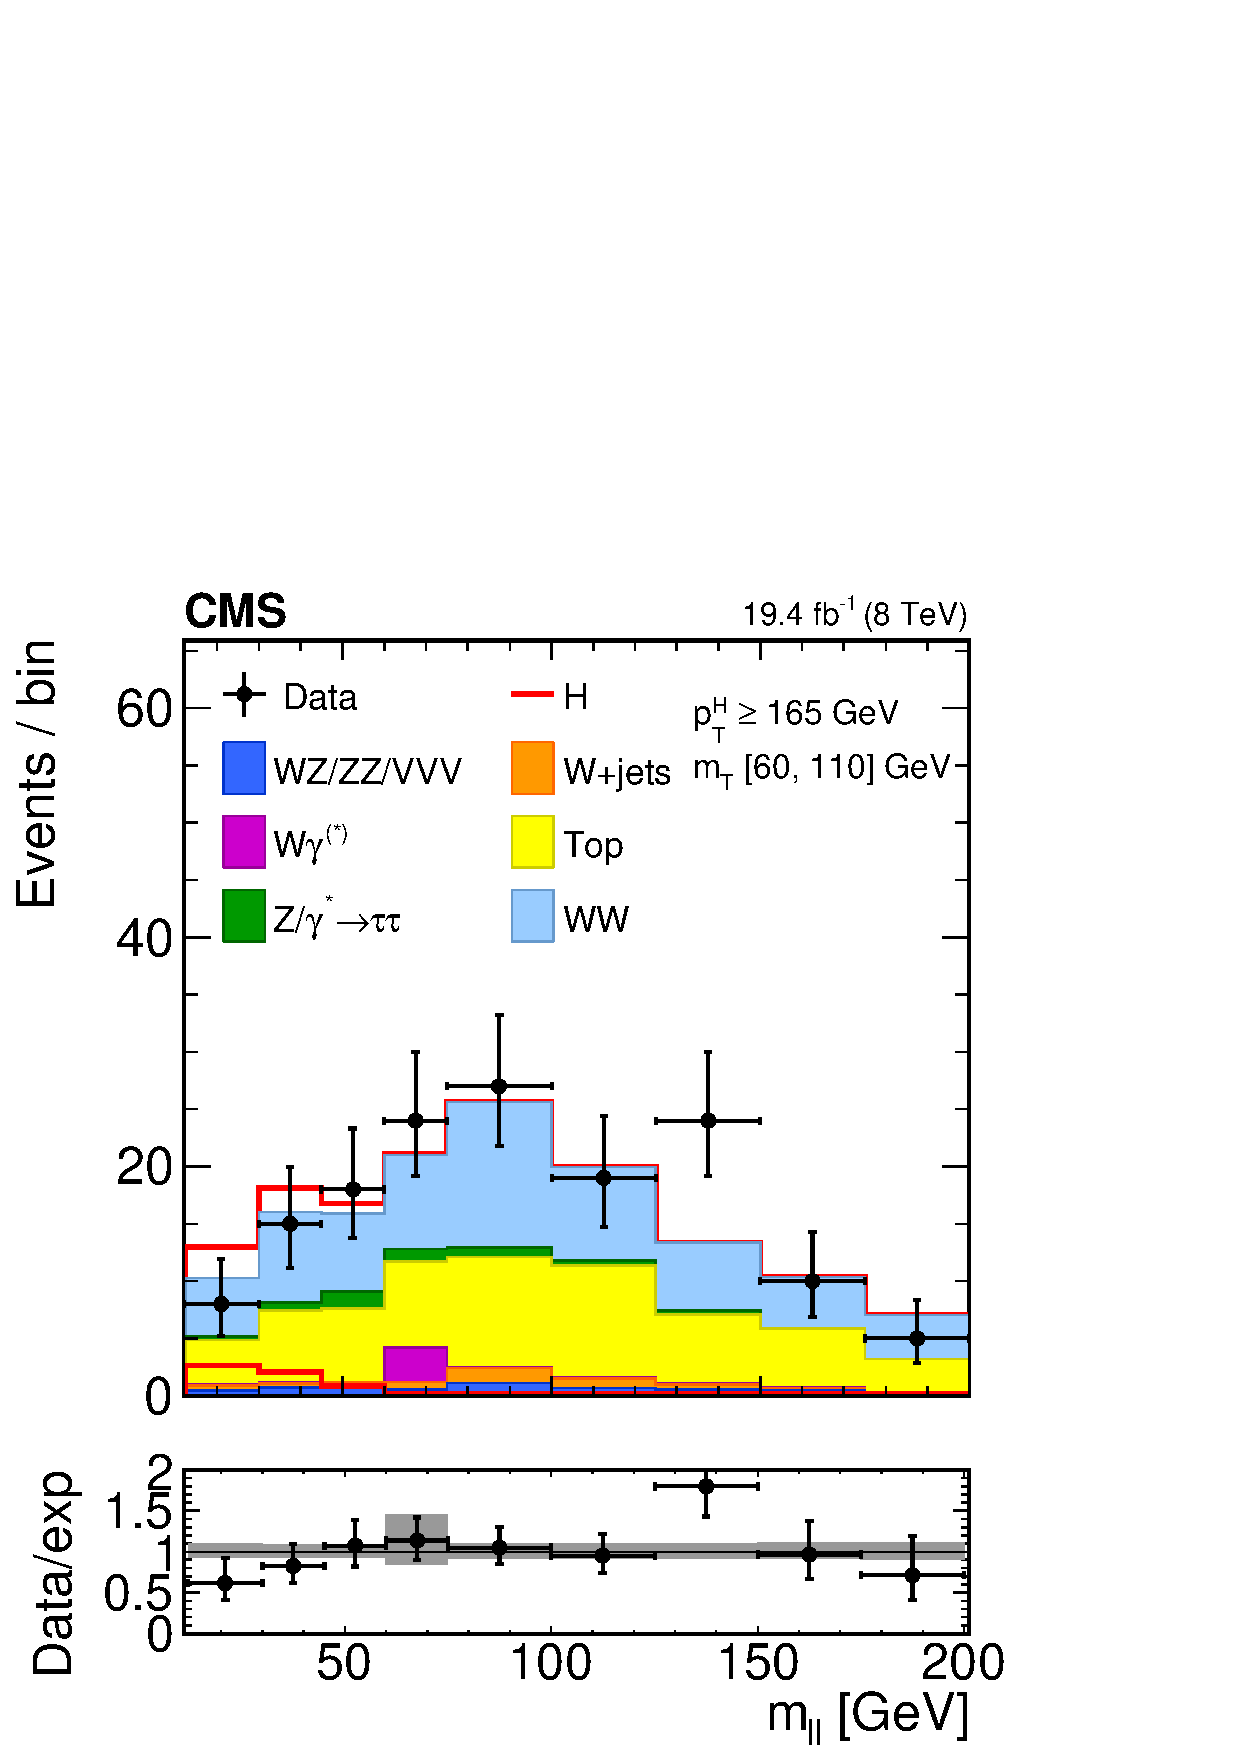
\includegraphics[width=0.45\textwidth]{images/WWnlo/mllBin5.pdf}}
\subfigure[\mll bin 6]{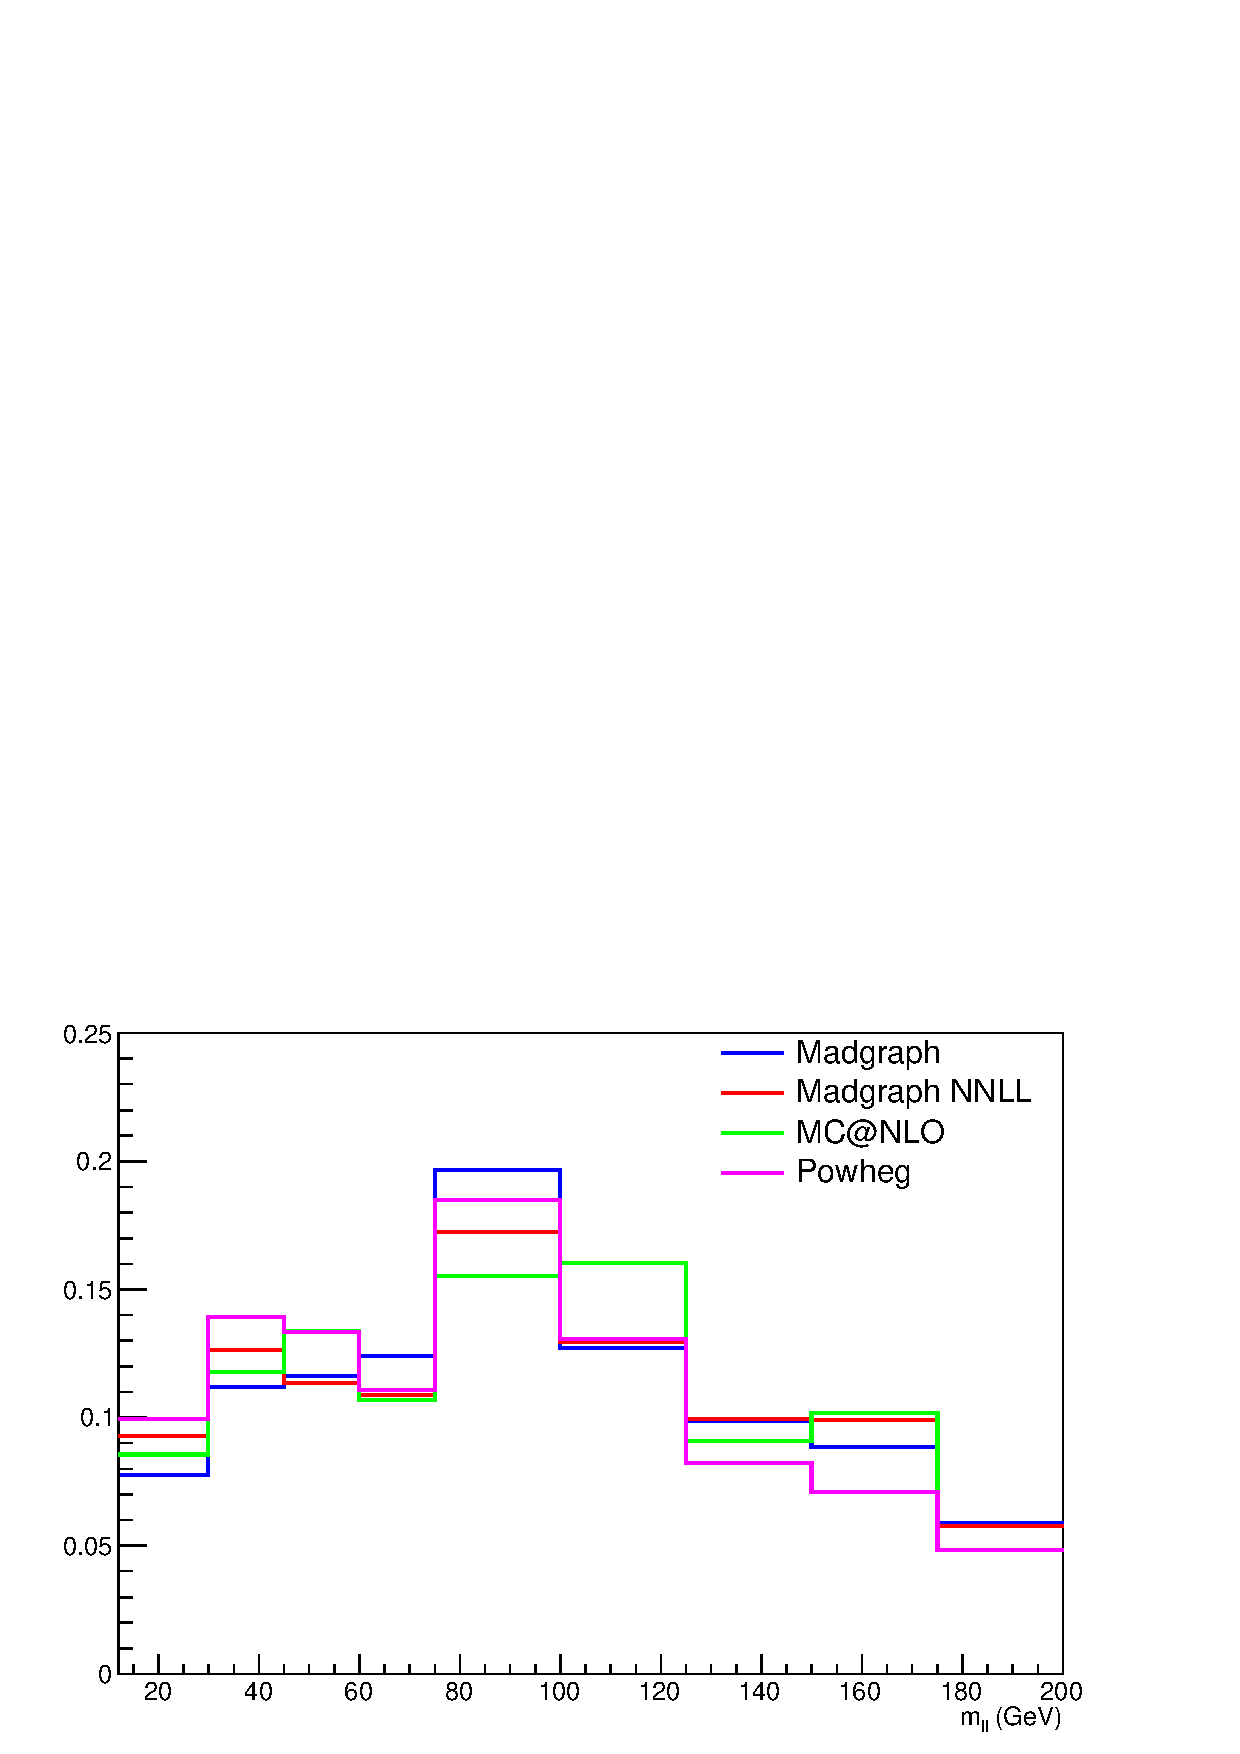
\includegraphics[width=0.45\textwidth]{images/WWnlo/mllBin6.pdf}}\\
\caption{Comparison between the default WW background sample and other theoretical models for the \mll distributions in every \pth bin.\label{fig:ww_mll}}
\end{figure}

\begin{figure}[htb]
\centering
\subfigure[\mt bin 1]{\includegraphics[width=0.45\textwidth]{images/WWnlo/mthBin1.pdf}}
\subfigure[\mt bin 2]{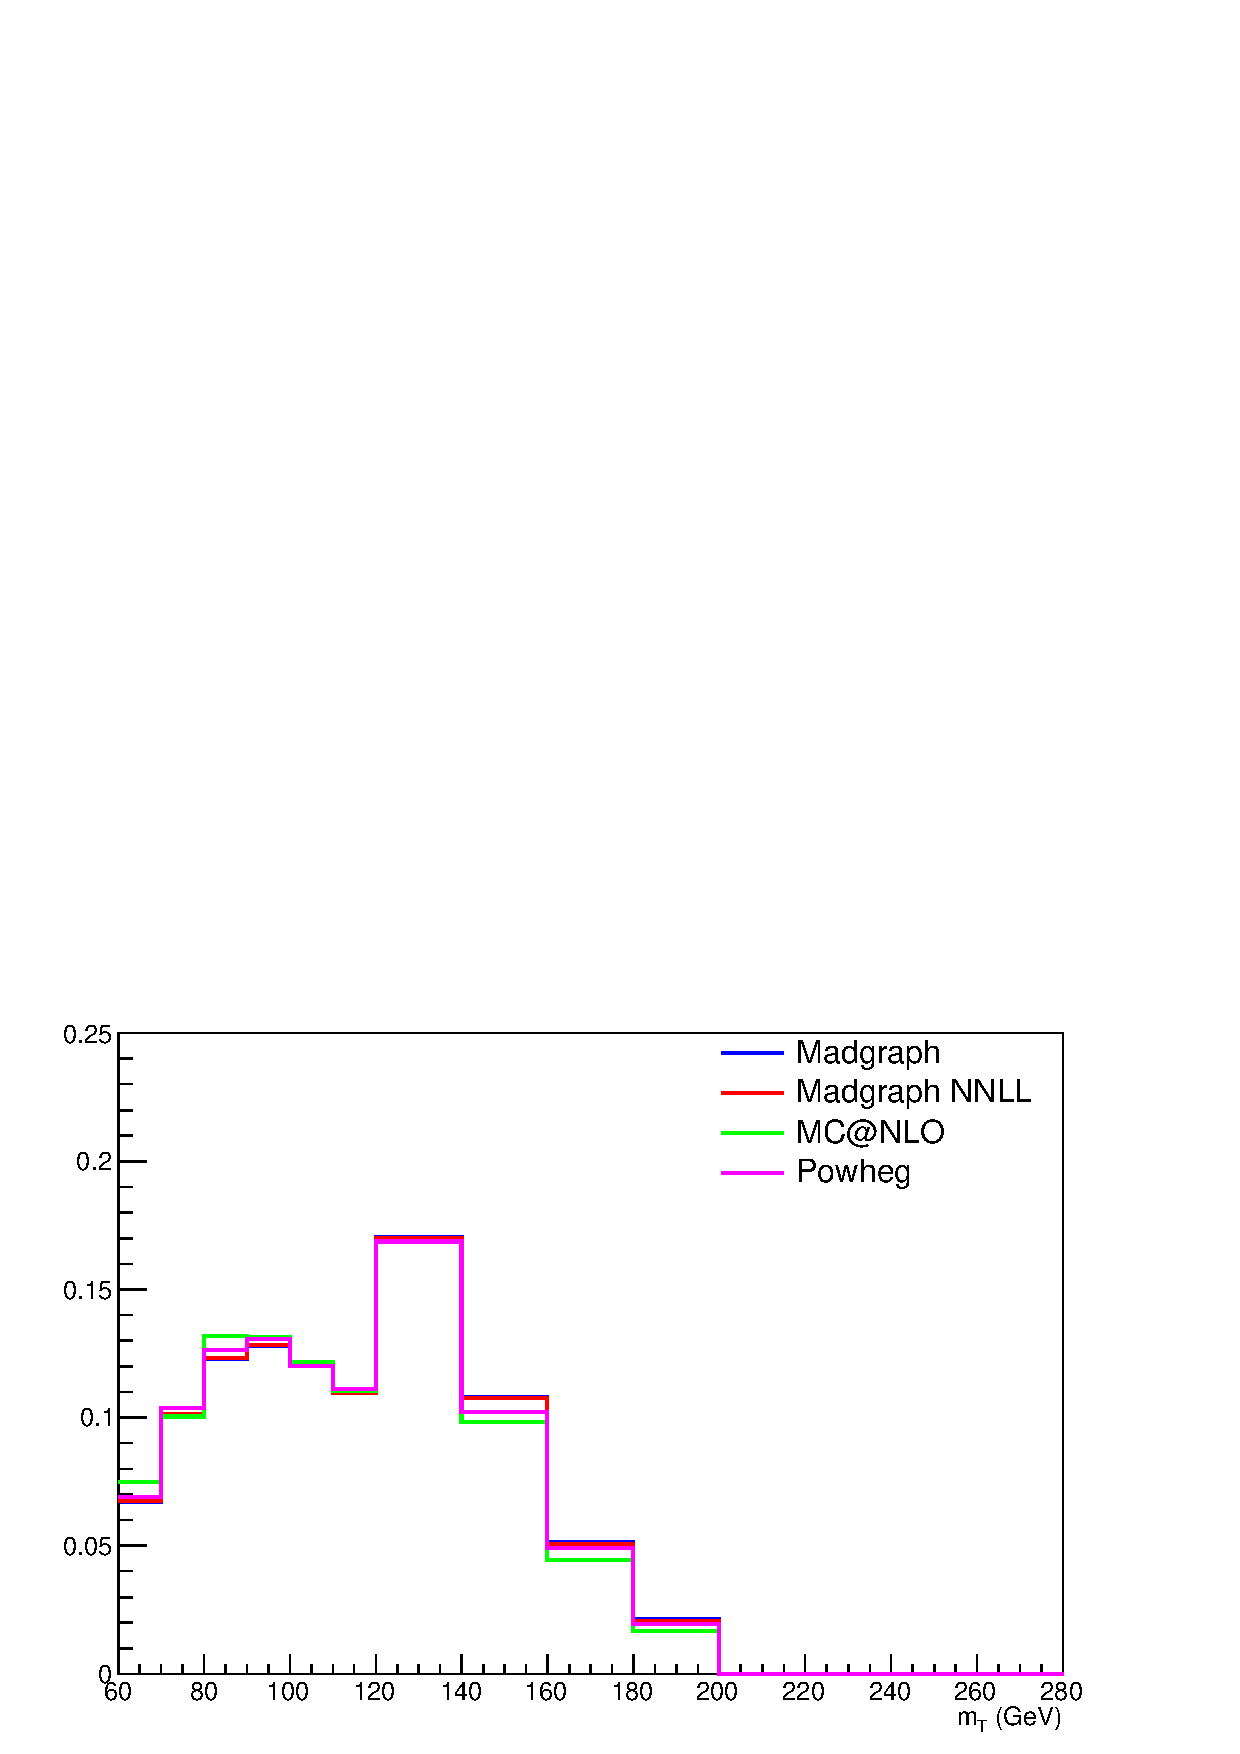
\includegraphics[width=0.45\textwidth]{images/WWnlo/mthBin2.pdf}}\\
\subfigure[\mt bin 3]{\includegraphics[width=0.45\textwidth]{images/WWnlo/mthBin3.pdf}}
\subfigure[\mt bin 4]{\includegraphics[width=0.45\textwidth]{images/WWnlo/mthBin4.pdf}}\\
\subfigure[\mt bin 5]{\includegraphics[width=0.45\textwidth]{images/WWnlo/mthBin5.pdf}}
\subfigure[\mt bin 6]{\includegraphics[width=0.45\textwidth]{images/WWnlo/mthBin6.pdf}}\\
\caption{Comparison between the default WW background sample and other theoretical models for the \mt distributions in every \pth bin.\label{fig:ww_mth}}
\end{figure}














































\subsection{Other backgrounds\label{sec:OtherBackgrounds}}

	%------------------------------------------------------------------------------------
	\subsubsection{W+jets background\label{sec:wjetsbkg}}	
Backgrounds containing one or two fake leptons are estimated from events
selected with relaxed lepton quality criteria, using the efficiencies for
real and fake leptons to pass the tight lepton quality cuts of the analysis. 

A data-driven approach, described in detail in~\cite{AN-2010-261} and~\cite{AN-2010-397}, is pursued 
to estimate this background. A set of loosely selected lepton-like objects, referred to as the 
'fakeable object' or ``denominator'' from here on, is defined in a sample of events 
dominated by dijet production. The denominator object definition used in the full 2012
data is described in~\cite{AN-2012-378}.

To measure the fake rate we count how many fakeable objects pass the full lepton selection 
of the analysis, parametrized as a function of the phase space of the fakeable lepton, therefore 
it is extracted in bins of $\eta$ and p$_T$.


The ratio of the fully identified lepton, referred as ``numerator'', to the 
fakeable objects is taken as the probability for a fakeable object to fake a lepton:

\begin{equation} 
{\mbox Fake\ Rate } = \frac{\# of \ fully \ reconstructed \ leptons}{\# of \ fakeable \ objects} 
\end{equation}

It is then used to extrapolate from the loose leptons sample to a sample of leptons satisfying the  
full selection. 

The details of the method implementation can be found in~\cite{AN-2013-022}.
% and only final results are quoted
%here. The resultant background yield estimates at the \WW selection level are given in Table~\ref{tab:WjetsBackground}.
The systematic uncertainty is evaluated by varying the jet thresholds in the di-jet control sample, and by
performing a closure test in the same-sign data sample (see~\cite{AN-2013-022}). In both cases it is about 36\%.

	%-------------------------------------------------------------------------------
	\subsubsection{Drell-Yan to \texorpdfstring{$\tau\tau$}{tau tau} background\label{sec:DYtautaubkg}}


The low \MET threshold in e$\mu$ final state
requires the consideration of the contribution from 
\dytt\, that is infact estimated from data.
This is accomplished by using 
\dymm events and replacing muons with a simulated
$\tau\to l\nu_\tau\bar{\nu_e}$ decay \cite{AN-2011-020}.\\
After replacing muons from \dymm decays with simulated $\tau$ decays,
the set of pseudo \dytt events undergoes the reconstruction step.
 
Good agreement in kinematic distributions for this sample
and a Monte Carlo based \dytt sample is found.
The global normalization of pseudo \dytt events is 
checked in the low \mt spectrum where a rather pure
\dytt sample is expected.


	%-------------------------------------------------------------------------------
	\subsubsection{ZZ, WZ and W\texorpdfstring{$\gamma$}{gamma} backgrounds\label{sec:otherbkg}}

The WZ and ZZ backgrounds are partially estimated from data when the two
selected leptons come from the same Z boson. If the leptons come from different
bosons the contribution is expected to be small. The WZ component is largely
rejected by requiring only two high \pt isolated leptons in the event. 
%The missing energy requirement makes the ZZ~$\to 4\ell$ component almost negligible.
%As the extra lepton veto and the \met cuts do not remove the ZZ~$\to 2\ell 2\nu$
%decays, a non-negligible fraction of these events survives the selection for $ee$ and $\mu\mu$ channels only. 

The W+$\gamma^{(*)}$ background, where the photon decays to an electron-positron pair,
is expected to be very small, thanks to the stringent photon conversion
requirements.
 Since the WZ simulated sample has a generation level cut on the
di-lepton invariant mass ($m_{\ell\ell} >$ 12~\GeV) and the cross-section raises
quickly with the lowering of this threshold, a dedicated \textsc{Madgraph} sample has
been produced with lower momentum cuts on two of the three leptons
($\pt > 5$~\GeV) and no cut on the third one. The surviving contribution
estimated with this sample is still very small, and since the uncertainty on the
cross-section for the covered phase space is large, a conservative 100\%
uncertainty has been given to it. 
A $k$-factor for W+$\gamma^{*}$ of $1.5\pm0.5$ based on a dedicated measurement of 
tri-lepton decays, W+$\gamma^{*} \to e\mu\mu$ and W+$\gamma^{*} \to \mu\mu\mu$,
is applied~\cite{WGammaStarStudy}. 
The contribution of W+$\gamma^{(*)}$ is also
constrained by a closure test with same sign leptons on data, which reveals a
good compatibility of the data with the expected background.


%\clearpage
\section{Systematic uncertainties}
%%%%%%%%%%%%%%%%%%%%%%%%%%%%%%%%%%%%%%%%%%%%%%%%%%%%%%%%%%%%%%%%%%%%%%
\label{sec:Systematics}

Systematic uncertainties play an important role in this analysis where
no strong mass peak is expected due to the presence of undetected
neutrinos in the final state.  One of the most important sources of
systematic uncertainty is the normalization of the backgrounds that
are estimated on data control samples whenever is possible.

A summary of the main sources of systematic uncertainty and the corresponding estimate is reported in Table~\ref{tab:Systematics}. A detailed description of each source of systematic uncertainty is discussed in the following sections.

\begin{table}[h]
\small{
  \begin{center}
  \caption{Main sources of systematic uncertainties and their estimate. The
  first category reports the uncertainties in the normalization of background
  contributions. The experimental and theoretical uncertainties refer to the
  effect on signal yields. A range is specified if the uncertainty varies
  across the $\pth$ bins.}
  \label{tab:Systematics}
  \begin{tabular}{cc}
  \hline\hline
  \multicolumn{2}{c} {\bf{Uncertainties in backgrounds contributions}} \\
  \hline
  Source  & Uncertainty \\
  \hline
  $\rm{t\bar{t}}$, tW      & 20--50$\%$ \\
  W+ jets              & $40\%$ \\
  WZ, ZZ              & $4\%$ \\
  W$\gamma^{(*)}$  & $30\%$ \\
  \hline\hline
  \multicolumn{2}{c} {\bf{Effect of the experimental uncertainties on the signal and background yields}}\\
  \hline
  Source & Uncertainty\\
  \hline
  Integrated luminosity        & $2.6\%$ \\
  Trigger efficiency           & 1--2$\%$\\
  Lepton reconstruction and identification & 3--4$\%$\\
  Lepton energy scale          & 2--4$\%$ \\
  \MET modelling          & $2\%$ \\
  Jet energy scale             & $10\%$ \\
  Pileup multiplicity          & $2\%$ \\
  b mistag modelling	       & $3\%$ \\	
  \hline\hline
  \multicolumn{2}{c}{\bf{Effect of the theoretical uncertainties on signal yield}}\\
  \hline
  Source & Uncertainty \\
  \hline
  b jet veto scale factor              & 1--2$\%$\\
  PDF                                  & $1\%$ \\
  WW background shape                  & $1\%$\\
  \hline
  \end{tabular}
  \end{center}
}
\end{table}


%-------------------------------------------------------------------------------
\subsection{Background normalization uncertainties}
%-------------------------------------------------------------------------------

The signal extraction is performed subtracting the estimated backgrounds to the event counts in data.
This uncertainty depends on the background: 
  \begin{itemize}
    \item {\bf\boldmath \ttbar and tW backgrounds:} 
      The efficiency on jets b-tagging is estimated using the Tag\&Probe technique in data
      and simulation control regions, as explained in \ref{sec:TagAndProbe}. 
      A per-jet scale factor, which takes into account the possibly different efficiency of the anti b-tagging selection in data and simulation, 
      is computed by means of the efficiency measured with the Tag\&Probe method.
%      \begin{equation}
%      w_{b-tag}^{n} = \left( \frac{1-\epsilon_{b-tag}^{DATA}}{1-\epsilon_{b-tag}^{MC}} \right)^n
%      \end{equation}
%      where $w_{b-tag}^{n}$ is the weight applied to events in the signal region with $n$ true 
%      b-jets and $\epsilon_{b-tag}^{DATA}$ and $\epsilon_{b-tag}^{MC}$ are the per-jet b-tagging efficiencies measured in data and MC respectively. 
      The Tag\&Probe method has been used also to measure the mistag rates in data and simulation, which are the probability to b-tag a jet that is not produced by the hadronization of a b quark.
%      The mistag scale factor $w_{mistag}^{n}$ is evaluated as:
%      \begin{equation}
%      w_{mistag}^{n} = \left( \frac{1-\epsilon_{mistag}^{DATA}}{1-\epsilon_{mistag}^{MC}} \right)^n
%      \end{equation}
      These factors are used to reweigh the Top MC samples as explained in \ref{sec:TTBackground}. The uncertainties provided by the Tag\&Probe fit are then propagated to the factor $\alpha$ that is used in the top data driven estimation \ref{sec:DD}.
      These uncertainties are embedded in a systematic error that affects the shape of the Top background in each \pth bin.
      
      Provided that the simulated samples include both \ttbar and tW processes, a systematic uncertainty related to the tW$/$\ttbar fraction has been included.
      In fact, a relative variation of the contribution of these two processes could modify the shape of the MC sample, and is thus included as a shape uncertainty affecting the top quark background shape in each \pth bin in a correlated way. 
      %The associated uncertainty ($\sim$30\%) is 
      %shared between the statistical of the control sample and the 
      %systematic one.
 
    \item {\bf\boldmath W+jets background:} It is estimated with data control
      sample as described in Sec.\ref{sec:wjetsbkg}. With 19.4\ifb at 8 \TeV,
      the uncertainty receives similar contributions from statistics
      and systematic error (mainly jet composition differences
      between the fake rate estimation sample and the application
      sample), the total error being about 40\%, dominated by the closure
      test of the method on a same-sign control region.
 
    \item {\bf\boldmath WZ,ZZ,W$\gamma^{(*)}$ backgrounds:} those backgrounds, which are
      expected to give a small contribution, are estimated from
      simulation. Uncertainties on the cross sections
      reported in \cite{xsecSM,bib:ellis} are 4\% for WZ and 2.5\% for ZZ.
      A 30\% uncertainty is assigned to the $W\gamma$ \cite{WgammaXsec} yield and another 30\% on $W\gamma^{(*)}$ contribution according 
      to the uncertainty on the normalization study (see Sec.~\ref{sec:otherbkg}).
      
  \end{itemize}

%-------------------------------------------------------------------------------
\subsection{Experimental uncertainties \label{subsec:expsyst}}
%-------------------------------------------------------------------------------

The following experimental systematic sources have been taken into account:

\begin{itemize}
\item {\bf Luminosity:} Using the online luminosity monitoring CMS
  reached an uncertainty on the luminosity of 2.6\% at 8 \TeV.

\item {\bf Trigger efficiency.} The uncertainties for both electrons and muons
  are at 1-2\% level, which is added together to the lepton efficiency uncertainty.

\item {\bf Lepton reconstruction and identification efficiency:} 
   The lepton reconstruction and identification efficiencies are measured with the Tag\&Probe
   method in data. To correct for the difference in the lepton identification
   efficiencies between data and MC, a scale factor is applied to MC.
   The uncertainties resulting from this procedure on the lepton efficiencies are 4\% for electrons and 3\% for muons.

\item {\bf Muon momentum and electron energy scale:} 
  The momentum scale of leptons have relatively large uncertainties due to different detector effects. 
  For electrons a scale  uncertainty of 2\% for the barrel, and 4\% for the endcaps respectively, 
  is assigned. 
  For muons, a momentum scale uncertainty of 1.5\%, independent of its pseudorapidity,  is assigned. 

\item {\bf {\boldmath \MET} modeling:} 
  The \MET measurement is affected by the possible mis-measurement of 
  individual particles addressed above, as well as the additional contributions 
  from the pile-up interactions. 
  The effect of the missing transverse momentum resolution on the event selection
  is studied by applying a Gaussian smearing of 10\% on the $x$- and
  $y$-components of the missing transverse momentum. All correlated variables,
  like the transverse mass, are recalculated. 
  %The effect is found to be around 2\%.

\item {\bf Jet energy scale (JES) uncertainties:} 
  It affects both the jet multiplicity and the 
  jet kinematic variables, such as $m_\mathrm{jj}$.
  We estimate this uncertainty applying variations of the official
  jet uncertainties on the JES (which depend on $\eta$ and $\pt$ of the jet 
   \cite{JEC2012}) and
  compute the variation of the selection efficiency. %It turns out to be about 10\%.

\item {\bf b jets mistag modeling:}
     A fraction of signal events is rejected because erroneously identified as b jets by the b-tagging algorithms.
     The mistag rate, as measured with the Tag\&Probe technique described in Sec.~\ref{sec:TTBackground}, comes with an uncertainty due to different modeling of the b-tagging performance in data and simulation.
          
\item {\bf Pileup multiplicity:} Some of the variables used in the
  analysis are affected by the average number of pileup
  interactions. The simulated events have been reweighted according
  the instantaneous luminosity measured on data.
  The error in the average number of pileup interactions measured in data
  and the simulation of the modeling and physics aspects of the pileup simulation 
  gives an uncertainty of 5\% on the 
  distribution used in the reweighting procedure.
  This uncertainty is propagated through all
  the analysis, and the estimated uncertainty on the efficiency is 2\%.

\end{itemize}

%-------------------------------------------------------------------------------
\subsection{Theoretical uncertainties \label{subsec:thsyst}}
%-------------------------------------------------------------------------------

\begin{itemize}

\item {\bf QCD scale uncertainties:}
  The uncertainties on the total cross sections due to the choice of the renormalization and factorization scale are assigned to MC-driven backgrounds.
  For the signal processes these uncertainties are separated in two categories: those affecting the selection efficiency and those affecting the jet bin fractions.
  The effect of renormalization and factorization scale on the selection efficiency is of the order of 2\% for all processes.
  Although this analysis is inclusive in number of jets, the effect of the QCD scale variation on the jet bin migrations has to be taken into account because of the b-tagging veto efficiency. The efficiency of this selection depends on jet multiplicity and the effect of the QCD scale variation has been evaluated using the Stewart-Tackman method, as explained in \ref{subsec:stewart-tackman}.

\item {\bf PDFs uncertainties:} 
  The utilization of different PDF sets can affect both the normalization and the shapes of the signal contributions. The uncertainty related due to the variations in the choice of PDFs is considered following the PDF4LHC~\cite{Alekhin:2011sk,Botje:2011sn} prescription, using CT10, NNPDF2.1~\cite{Ball:2011mu} and MSTW2008~\cite{Martin:2009iq} PDF sets.


\item {\bf \boldmath{WW}:} 
  Due to the fact that the WW shape is entirely taken from simulation, the analysis is strongly
  relying on theoretical models and can thus be strongly affected by their uncertainties. Especially higher order QCD radiative effects have an influence on the generated WW shape. To study this impact, the shapes of the distributions produced with the \textsc{MadGraph} generator (which is the generator for the MC simulation used in the analysis) are compared to the ones produced with \textsc{mc@nlo}. The comparison is performed separately in each bin of \pth and the uncertainty includes shape differences originating from the renormalization and factorization scale choice. A comparison of the \mll and \mt shapes for the WW background using different MC generators is reported in section \ref{sec:WWBackground}.
\end{itemize} 

\subsubsection{Jet multiplicity uncertainty \label{subsec:stewart-tackman}}

The jet bin uncertainty on the ggH production mode has been evaluated using the Stewart-Tackman method, following the recipe proposed in Refs.~\cite{Stewart:2011cf,Heinemeyer:2013tqa}.
Three independent nuisance parameters have to be associated with the inclusive ggH production cross sections $\sigma_{\geq 0}$, $\sigma_{\geq 1}$ and $\sigma_{\geq 2}$, which corresponds to the cross sections with $\geq 0$ jets, $\geq 1$ jet and $\geq 2$ jets respectively. According to the agreement on the treatment of uncertainties in the combination of ATLAS and CMS results~\cite{ATLAS:2011tau}, these nuisance parameters are labelled as \emph{QCDscale\_ggH}, \emph{QCDscale\_ggH1in} and \emph{QCDscale\_ggH2in}. However, in case the analysis is split in exclusive jet multiplicity bins, the jet bin uncertainties can be evaluated taking into account the correct correlations among the three nuisances following the Stewart-Tackman prescription.
Even though this analysis is inclusive in number of jets, the jet binning uncertainties must be included due to the presence of the b-jet veto, that introduces a dependency of the selection efficiency on the number of jets in the event. The veto efficiency has been evaluated in all the \pth bins defined in the analysis and as a function of jets multiplicity. The results are shown in Figs.~\ref{fig:veto_eff_pth} and \ref{fig:veto_eff_njet}. The drop of the veto efficiency at high values of \pth is due to the correlation with jets multiplicity.
	 	
\begin{figure}[htb]
\centering
	\subfigure[]{
		\centering
		\includegraphics[width=0.45\textwidth]{images/eff_vs_pth.pdf}
		\label{fig:veto_eff_pth}
	}
	\subfigure[]{
		\centering
		\includegraphics[width=0.45\textwidth]{images/eff_vs_jet.pdf}
		\label{fig:veto_eff_njet}
	}
\caption{(a) Efficiency of the b-tagging veto in different bins of \pth. (b) Efficiency of the b-tagging veto in different bins of \pth, as a function of number of jets.}
\end{figure}

The first step of this procedure is to take the inclusive ggH cross section, $\sigma_\mathrm{ggH}$, and to convert the relative QCD up/down scale uncertainties, $\epsilon_+$ and $\epsilon_-$, to a log-normal uncertainty, i.e. $\kappa = \sqrt{\exp{(\epsilon_+)}\cdot \exp{(\epsilon_-)}}$. The exclusive cross sections, $\sigma_0$, $\sigma_1$ and $\sigma_2$, can be calculated starting from $\sigma_\mathrm{ggH}$ and using the selection efficiencies for the three jet bins. For every exclusive cross section the corresponding relative uncertainty is computed varying the renormalization ($\mu_R$) and factorization ($\mu_F$) scales independently of a factor 2 and $1/2$, and taking the cross section value corresponding to half of the maximum variation. The inclusive cross sections are then obtained summing the exclusive cross sections and propagating the uncertainties, i.e. $\sigma_{\geq 0 } = \sigma_0 + \sigma_1 + \sigma_2$, $\sigma_{\geq 1} = \sigma_1 + \sigma_2$, $\sigma_{\geq 2} = \sigma_2$.

The three nuisance parameters, including all the proper correlations among the jet bins, are defined according to Table~\ref{table:jet_binning_theory}, where the $f_n$ constants represent the exclusive theoretical $n$ jet bin fractions, i.e. $f_0 = \sigma_0/\sigma_{\geq 0}$, $f_1 = \sigma_1/\sigma_{\geq 0}$, $f_2 = \sigma_2/\sigma_{\geq 0}$.

\begin{table}[h]
\caption{Numerical calculation for the systematic uncertainties of jet binning.}
\label{table:jet_binning_theory}
\begin{center}
\begin{tabular}{|l|c|c|c|}
\hline
Nuisance parameter & 0-jet bin                                              & 1-jet bin                                            & 2-jet bin \\ 
\hline
&&& \\
QCDscale\_ggH          & $\Delta^0_{\geq 0} = (\kappa_{\ge 0})^{\frac{1}{f_0}} $    &      & \\ 
&&&\\\hline
&&&\\
QCDscale\_ggH1in       & $\Delta^0_{\geq 1} = (\kappa_{\ge 1})^{- \frac{f_1 + f_2}{f_0}} $ & $\Delta^1_{\geq 1} = (\kappa_{\ge 1})^{\frac{f_1 + f_2}{f_1}} $ & \\ 
&&&\\ \hline
&&&\\
QCDscale\_ggH2in        &                                                        & $\Delta^1_{\geq 2} = (\kappa_{\ge 2})^{- \frac{f_2}{f_1}} $     & $\Delta^2_{\geq 2} = (\kappa_{\ge 2})$ \\ 
&&&\\\hline

\end{tabular}
\end{center}
\end{table}

The nuisance parameters reported in table \ref{table:jet_binning_theory} have then been calculated for each \pth bin embedding the b-jet veto efficiency and using the following formulas:
\begin{equation}
\emph{QCDscale\_ggH}=\frac{\Delta^0_{\geq 0}\cdot f_{0}\cdot \varepsilon_{0}+\Delta^0_{\geq 1}\cdot f_{1}\cdot\varepsilon_{1}}{\Delta^0_{\geq 0}\cdot f_{0}\cdot \varepsilon_{0}+\Delta^0_{\geq 1}\cdot f_{1}\cdot \varepsilon_{0}} \quad,
\end{equation}
\begin{equation}
\emph{QCDscale\_ggH1in}=\frac{\Delta^1_{\geq 1}\cdot f_{1}\cdot \varepsilon_{1}+\Delta^1_{\geq 2}\cdot f_{2}\cdot \varepsilon_{2}}{\Delta^1_{\geq 1}\cdot f_{1} \cdot \varepsilon_{1}+\Delta^1_{\geq 2}\cdot f_{2}\cdot \varepsilon_{1}} \quad,
\end{equation}
\begin{equation}
QCDscale\_ggH2in=1 \quad,
\end{equation}
where $\varepsilon_0$, $\varepsilon_1$ and $\varepsilon_2$ are the selection efficiencies for the three jet categories.
These nuisance parameters are expected to be equal to one in case the efficiency is independent on the number of jets, i.e if $\varepsilon_0 = \varepsilon_1 = \varepsilon_2$.\\
The numerical values obtained following this procedure are reported in Table~\ref{table:jet_binning_meas} for each \pth bin.

\begin{table}[h]
\caption{Values of the jet binning nuisance parameters for different \pth bins.}
\label{table:jet_binning_meas}
\begin{center}
\begin{tabular}{ccccccc}
\toprule
\multirow{2}{*}{Nuisance parameter} & \multicolumn{6}{c}{\pth bin [GeV]} \\
& [0-15] & [15-45] & [45-85] & [85-125] & [125-165] & [165-$\infty$]\\
\midrule
QCDscale\_ggH  & 0.998  &   0.993  &   0.989  &   1.000  &   1.000   &  1.000 \\
QCDscale\_ggH1in &0.997   &  0.993  &   0.984  &   0.975 &    0.946 &    0.974  \\
\bottomrule
\end{tabular}
\end{center}
\end{table}


%-------------------------------------------------------------------------------
\subsection{Statistics uncertainty of the simulated samples}
%-------------------------------------------------------------------------------

Due to the large range of weights used to correct the simulated distributions in order to
match those in data, the effective size of the MC samples are sometimes smaller than
the actual number of events in the sample.
The statistical uncertainties of the event yields estimated from MC samples
are included as nuisance parameters in the fit and have a small impact on the final result.

%-------------------------------------------------------------------------------
\subsection{Treatment of systematic uncertainties in the shape analysis}\label{sec:syst_treatment}
%-------------------------------------------------------------------------------

One can distinguish between normalization uncertainties, where a systematic
effect is changing the normalization of a given process assuming the shape is not affected, and
shape uncertainties where the actual change in the shape of the distribution is
taken into account. The normalization uncertainties enter the shape analysis as
a constant normalization factor, whereas for shape uncertainties the nominal and
the $+1\sigma$ and $-1\sigma$ shapes enter the analysis in form of three histograms
with the same normalization. 

For the W+jets background, the shape differences for different jet \pt thresholds in the 
di-jet control sample are considered separately for electron and muon fakes, while the
other sources of systematics are taken as normalization uncertainties as in the cut-based
analysis.

Effects from experimental uncertainties are studied by applying a scaling and smearing of certain variables of the physics objects, followed by a subsequent
recalculation of all the correlated variables. This is done for simulation, to account for possible systematic mis-measurements of the data.
All experimental sources from Section~\ref{subsec:expsyst} but luminosity
are treated both as normalization and shape uncertainties.
For background with a data-driven normalization estimation,
only the shape uncertainty is considered.

To account for statistical uncertainties, for each distribution going into the shape analysis, 
the $+1\sigma$ and $-1\sigma$ shapes were obtained by adding/subtracting the statistical error 
in each bin and renormalizing it to the nominal distribution. In addition to this procedure a constant 
normalization uncertainty due to the finite statistics of the MC sample used to extract the shape is assigned.


%\clearpage
\section{Signal Extraction}
%%%%%%%%%%%%%%%%%%%%%%%%%%%%%%%%%%%%%%%%%%%%%%%%%%%%%%%%%%%%%%%%%%%%%%
\label{sec:SignalExtraction}
The signal is extracted in each bin of \pth by using a 2D template for signals and backgrounds in the \mll-\mt plane. This is the same strategy used in the main WW analysis. 
The binning of the \mll and \mt templates is:
\begin{itemize}
\item {\mll: $[12,30,45,60,75,100,125,150,175,200]$} 
\item {\mt: $[60,70,80,90,100,110,120,140,160,180,200,220,240,280]$}
\end{itemize}
We have checked that these two variables are not correlated with \pth, as shown in Fig.~\ref{fig:correlation_ggH} and Fig.~\ref{fig:correlation_vbf} for gluon fusion and VBF signals respectively.
\begin{figure}[htb]
\centering
\subfigure[]{\includegraphics[width=0.45\textwidth]{images/correlationmll_ggH.pdf}}
\subfigure[]{\includegraphics[width=0.45\textwidth]{images/correlationmth_ggH.pdf}}
\caption{Correlation between $\pth$ and $\mll$ (a) and between \pth and \mt (b) after the full selection for the gluon fusion signal.\label{fig:correlation_ggH}}
\end{figure}

\begin{figure}[htb]
\centering
\subfigure[]{\includegraphics[width=0.45\textwidth]{images/correlationmll_vbf.pdf}}
\subfigure[]{\includegraphics[width=0.45\textwidth]{images/correlationmth_vbf.pdf}}
\caption{Correlation between \pth and \mll (a) and between \pth and \mt (b) after the full selection for the VBF signal.\label{fig:correlation_vbf}}
\end{figure}

The signal extraction is performed using the {\tt combine} tool. 
We have defined a model with six signal strength parameters, one for each bin.
The relative contribution for different production mechanisms in the input signal template is taken to be the same as the SM.
The signal strength in each bin is allowed to float between -10 and +10, thus allowing negative values. This is mainly intended to allow the error bars to float below 0.\\
The fake events, i.e. reconstructed events not belonging to the fiducial region, are included in the signal definition. In fact in this step we are extracting all the events passing the analysis selection, regardless of the fiducial region definition.
Those events must be subtracted before the unfolding: to do this, given the fiducial region, we have computed the expected spectrum of fake events in bins of \pth. Then each bin of the spectrum is multiplied by the measured signal strength in that bin and then subtracted from the measured spectrum.
At the end, the number of events in each bin $i$ of the measured spectrum is:
\begin{equation}
N_i = \mu_i (s_i -f_i) \quad ,
\end{equation}
where $s_i$ and $f_i$ are respectively the number of signal and fake events expected from MC and $\mu_i$ is the measured signal strength.

\subsection{Fitting procedure}\label{subsec:fit}
The fit is a binned likelihood fit. Each source of systematic uncertainty is represented by a nuisance parameter in the fit.
Each signal is splitted in the six different bins of \pth as shown also in the yields table \ref{table:yields}. The WW and Top backgrounds have been also splitted in the various bins of Higgs \pt in order to reduce a possible shape mismatching between data and MC.\\
The fit is not performed on data, being the analysis is still blinded, but rather on a toy Asimov dataset. The best fit parameters values and the related profile-likelihood uncertainties extracted from the fit including all the nuisances in the model are shown in table \ref{table:fit_full}. For each parameter of interest the MINOS algorithm has been used.

\begin{table}
\centering
\caption{Best fit values and profile-likelihood uncertainties for all the signal strengths obtained fitting all the nuisances in the model.}\label{table:fit_full}
\begin{tabular}{c|c|c}
\hline
Signal strength & Best fit value & Uncertainty (68\% C.L.)\\
\hline\hline
$\mu_0$ & 1.000 & -0.408/+0.421 \\
$\mu_1$ & 1.000 & -0.294/+0.305 \\
$\mu_2$ & 1.000 & -0.420/+0.441 \\
$\mu_3$ & 1.000 & -0.860/+0.913 \\
$\mu_4$ & 1.001 & -1.224/+1.380 \\
$\mu_5$ & 1.001 & -0.932/+1.091 \\
\hline
\end{tabular}
\end{table}

In order to assess the robustness of the fit we have also run on several toy MC with a statistics corresponding to the one expected in data. The distribution of the signal strengths extracted in each bin in the toys and the their pulls are shown in Fig.~\ref{fig:pull_fit}. 
\begin{figure}[htb]
\centering
\subfigure[]{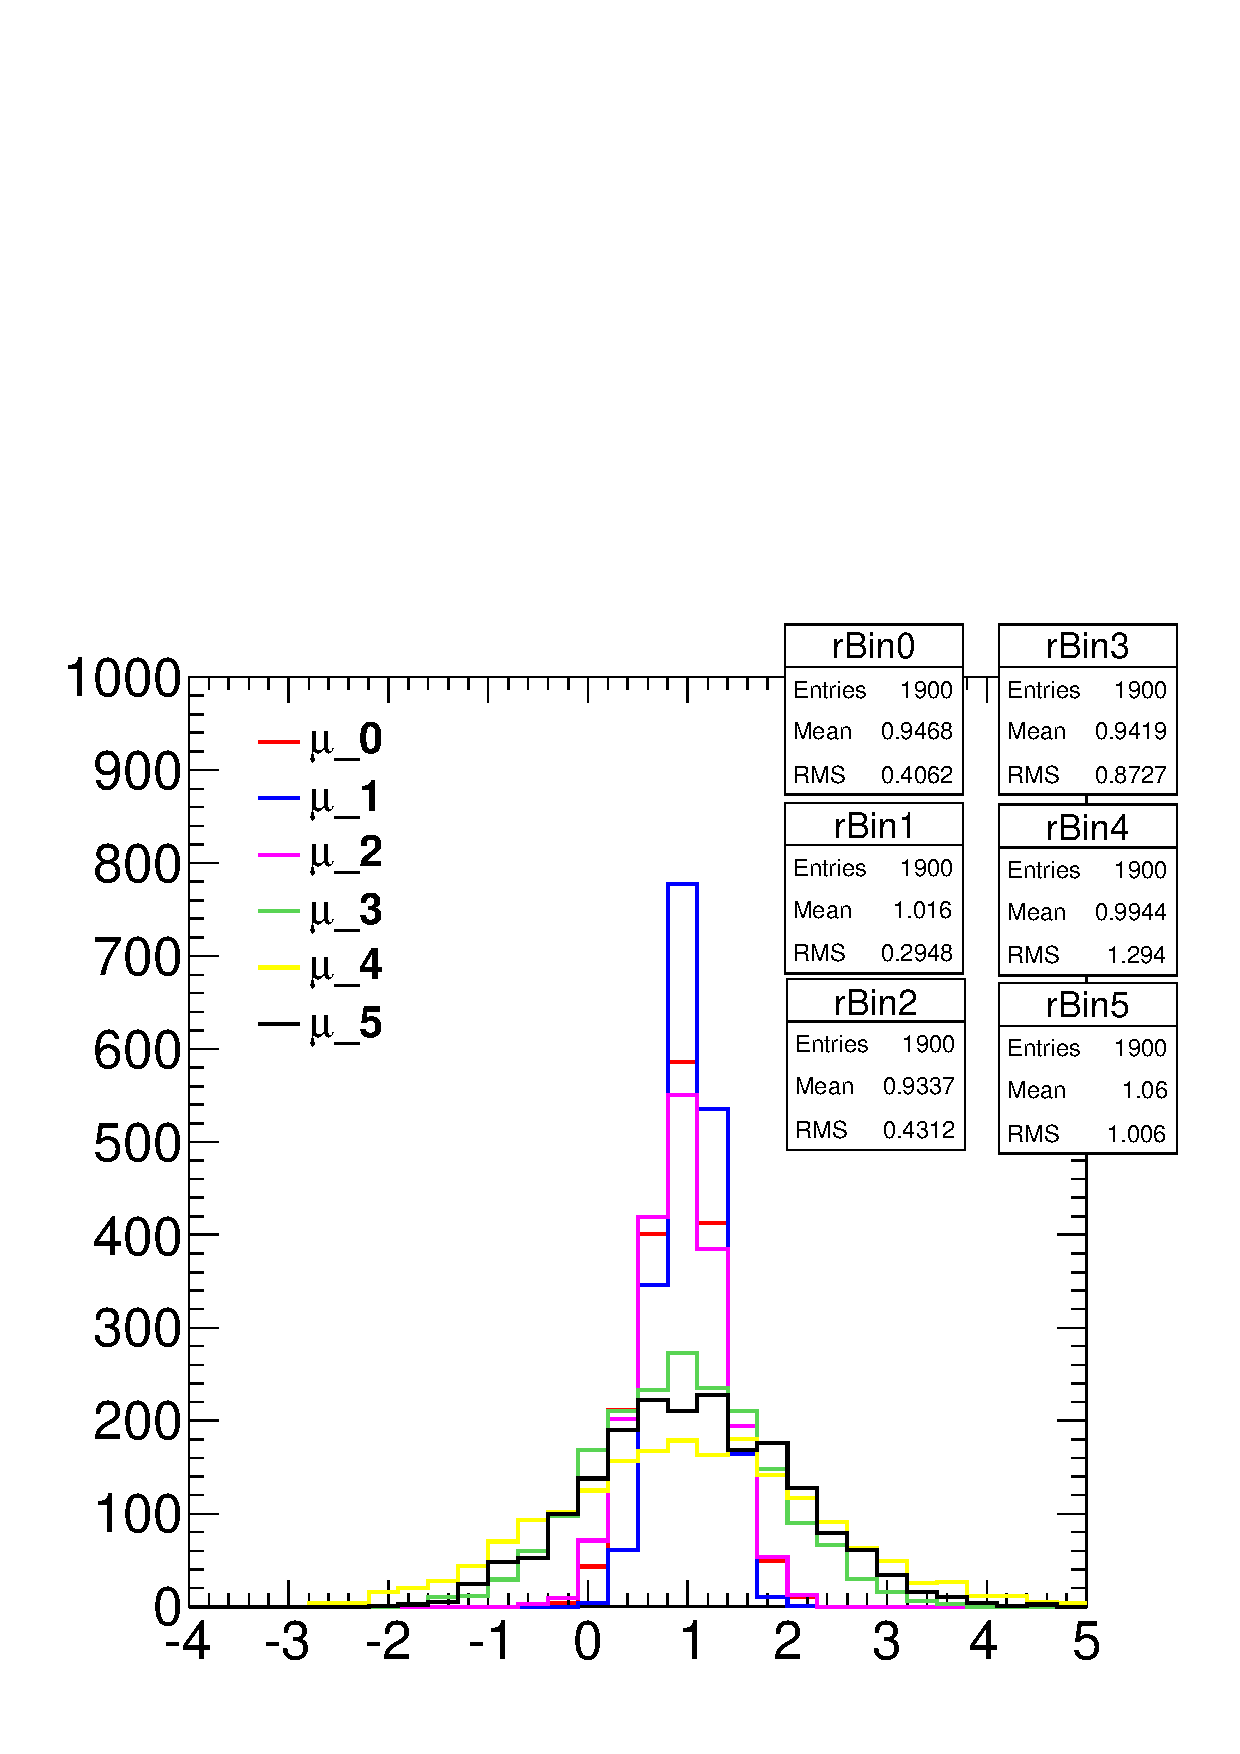
\includegraphics[width=0.45\textwidth]{images/mu_toys.pdf}}
\subfigure[]{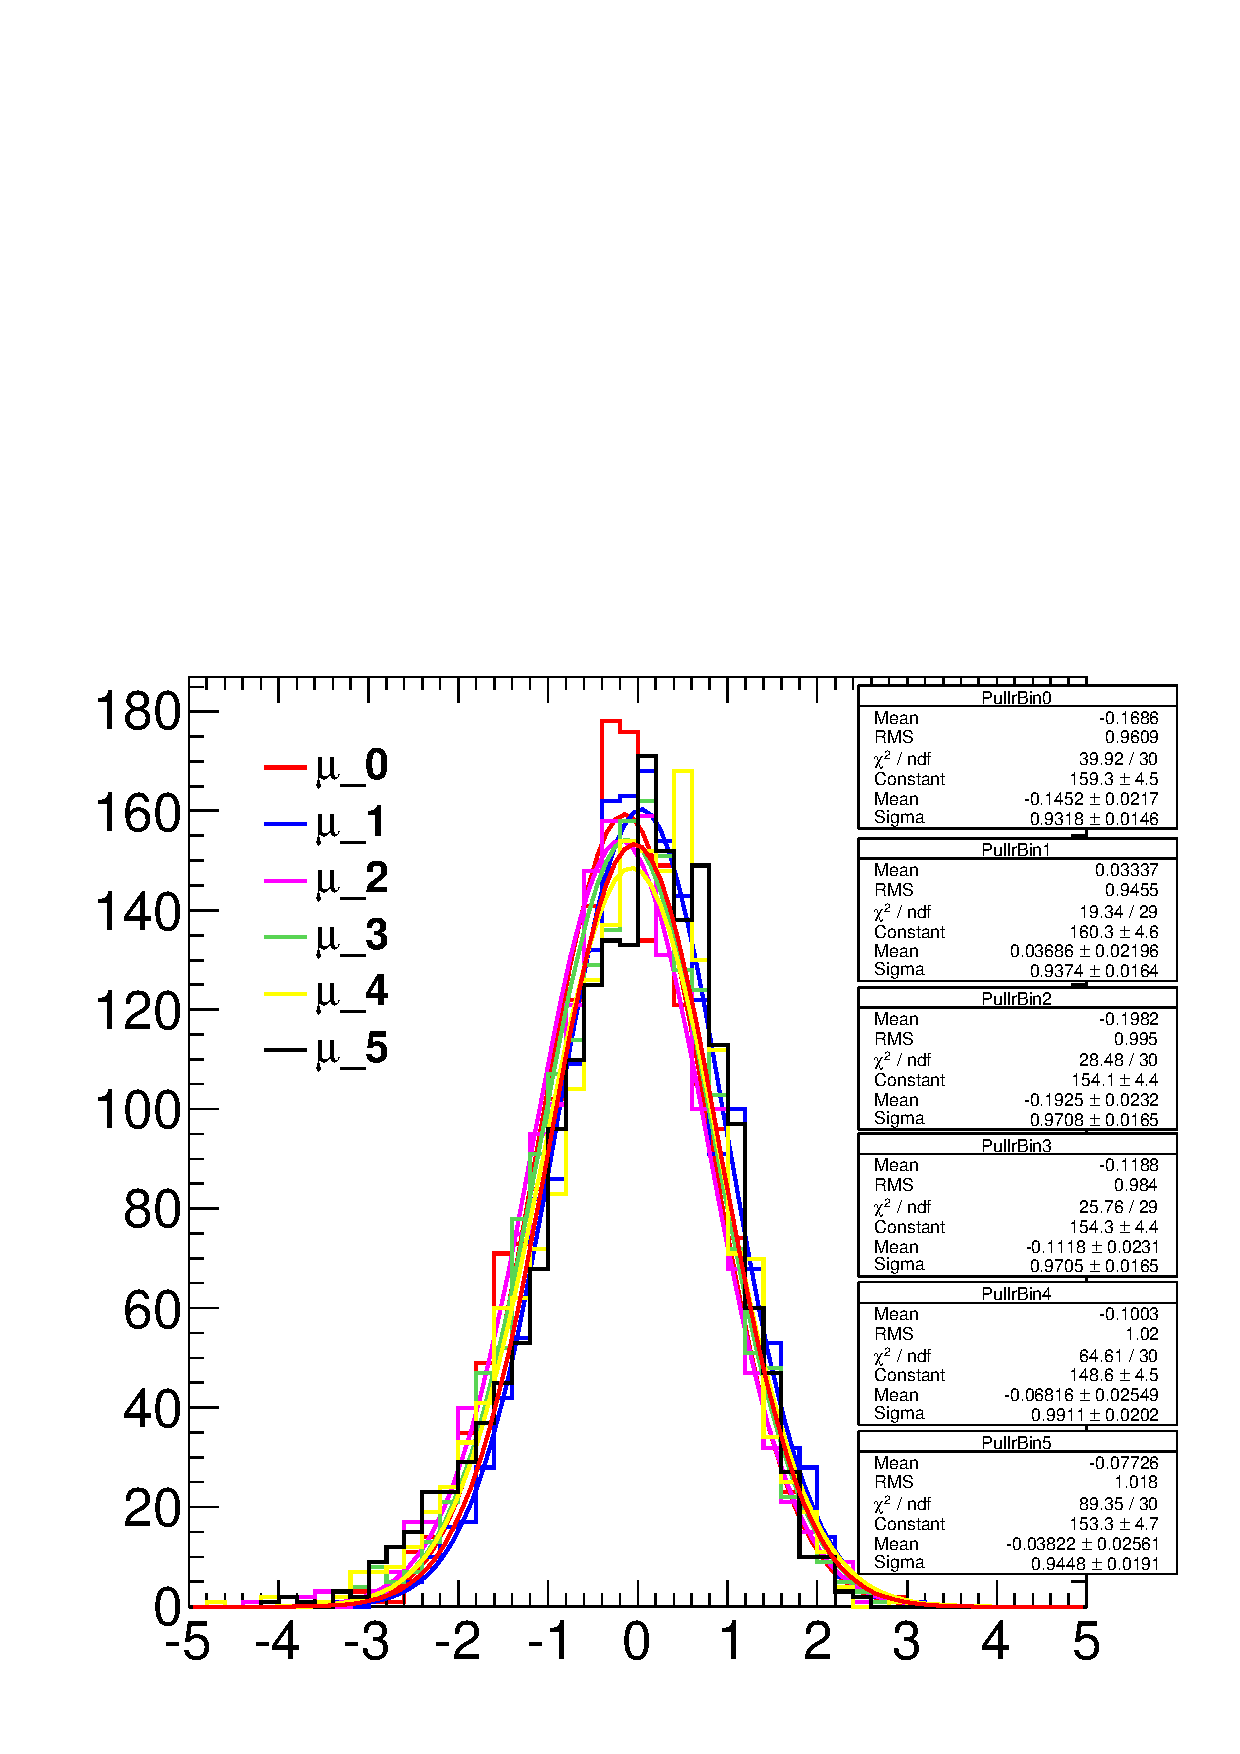
\includegraphics[width=0.45\textwidth]{images/pull_toys.pdf}}
\caption{Signal strengths distribution as extracted from the fit in toy MC (a). Pulls of the signal strength parameters (b).\label{fig:pull_fit}}
\end{figure}

%\clearpage
\section{Unfolding}
%%%%%%%%%%%%%%%%%%%%%%%%%%%%%%%%%%%%%%%%%%%%%%%%%%%%%%%%%%%%%%%%%%%%%%
\label{sec:Unfolding}
In order to report the results in such a way that is easy to make a comparison with theoretical prescriptions or with other experiments results, the signal extracted performing the fit has to be corrected for detector resolution and efficiency effects and for the efficiency of the selection defined in the analysis.\\
To achieve this an unfolding procedure has been set up relying on the \textit{RooUnfold}~\cite{Adye:2011gm} package which provides the tools to run various unfolding algorithms.\\
The results are extrapolated to a fiducial region defined using generator level variables, as discussed in section \ref{sec:AnalysisStrategy}, in particular using  the status three definition for leptons, which identifies the ``hard part'' of the interaction, i.e. the partons that are used in the matrix element calculation, including immediate decays of resonances.
For this 8~\TeV analysis, in which the uncertainty is dominated by the low statistics, the effect of unfolding to status three particles (which are, strictly speaking, not observable) instead of status one (i.e. what one would observe with a perfect detector) are expected to be negligible.\\
The basic principle behind the unfolding procedure is to use MC signal samples to make the ``true'' distribution (the one obtained with MC truth information) of the variable of interest and the same distribution obtained with events reconstructed after the full GEANT4 simulation of the CMS detector and event reconstruction. These two distributions are used to calculate the response matrix $M$, given by:
\begin{equation}
R_i^{MC} = M_{ij}T_j^{MC} \quad ,
\end{equation}
where $R^{MC}$ and $T^{MC}$ are two n-dimensional vectors (where n is the number of bins of the distribution) representing the reconstructed distribution and to the true distribution respectively.\\
The response $M [n \times n]$ matrix includes all the effects related to the detector and to the analysis selection that affect the $R^{MC}$ distribution.\\
The goal of the unfolding procedure is to go back to the true distribution starting from the measured one. The most natural way to achieve this would be inverting the response matrix. However it can be shown~\cite{Cowan} that, due to the finite statistical accuracy of the response matrix, which is limited by the MC statistic, a simple inversion could lead to huge fluctuations between bins in the unfolded result. Regularization methods can however be employed to make the matrix inversion well behaved. Several methods are implemented in the RooUnfold package, and they all depend on the choice of a regularization parameter. The choice of the regularization parameter is particularly critical, and it should represent an optimal trade-off between taming the fluctuations in the unfolded result, and biasing the unfolded distribution towards the one used to build the response matrix. 

\subsection{Response matrix}
The first step is to build the response matrix.
The matrix is built as two-dimensional histograms, plotting the generator level Higgs \pt on the $x$ axis and the same variable at reconstructed level on the $y$ axis. For both the generator and reconstruction level variable the same binning has been chosen following the prescription described in section \ref{sec:Binning}.
Both fake events, i.e. events reconstructed in a given bin without a generated counterpart, and miss events, i.e. events generated in a given bin but not reconstructed, are taken into account in order to build the response matrix.
In figure \ref{fig:response_matrix} the response matrix is shown, either normalized by column or by row, in order to show respectively the purity and the stability values in the diagonal bins. The fake events distribution is shown in figure \ref{fig:fakes}. 
\begin{figure}[t]
\centering
\subfigure[]{
\includegraphics[width=0.45\textwidth]{images/response_matrix_newACC_purity.pdf}
}
\subfigure[]{
\includegraphics[width=0.45\textwidth]{images/response_matrix_newACC_stability.pdf}
}
\caption{Response matrix normalized to one either by column (a) or by row (b).}
\label{fig:response_matrix}
\end{figure}

\begin{figure}[b]
\centering
\includegraphics[width=0.6\textwidth]{images/fakes.pdf}
\caption{Fakes distribution, i.e. events reconstructed in a given bin without any generator level event associated, normalized to the data luminosity.}
\label{fig:fakes}
\end{figure}

\subsection{Regularization method}\label{sec:regularization}
In this analysis we used the SVD (Singular Value Decomposition) tool based on Tikhonov regularization function, provided within the \textit{RooUnfold} package. The choice of the regularization parameter follows the prescription in~\cite{Hocker:1995kb}. The prescription proceeds as follows: one needs to diagonalize the response matrix with the SVD decomposition and plot, as a function of the bin number, the values of a transformed vector called $d_{i}$ which represents the measured distribution in a specific base defined by the SVD decomposition. The optimal choice for the regularization parameter is a value that corresponds to where the curve becomes flat around 1.    
This choice is data driven and will have to be re-evaluated after the unblinding of the data. 
For the moment we have performed the test on the Monte Carlo, as shown in Fig.~\ref{fig:log_di}, and we decided to use a value of 3.
The test has been performed using 200 toy MC samples and calculating for each one of them the $\log{d_i}$ function. The values in each bin $i$ correspond to the mean values obtained from the toys and the corresponding errors.
However, the final choice of the regularization parameter has to be done looking at data after the unblinding.

\begin{figure}[htb]
\centering
\includegraphics[width=0.6\textwidth]{images/logdi_good.pdf}
\caption{Trend of the $\log{d_i}$ function as a function of $i$. The curve flattens for a value $i=3$, used as regularization parameter.}
\label{fig:log_di}
\end{figure}

In order to show the unfolded spectrum dependence on the choice of the regularization parameter, the unfolded procedure has been repeated for several regularization values. The various plots are shown in figure \ref{fig:kreg_test} for regularization values varying from 1 (stronger regularization) to 5 (weaker regularization). Using $k_{reg} = 6$ is equivalent to the simple inversion of the response matrix and leads to huge errors. Lowering $k_{reg}$ means increasing the regularization and thus reducing the statistical uncertainty. One should increase the regularization as much as possible until the procedure starts to bias the distribution. The distribution starts to be biased, according to the $\log{d_i}$ curve criterion, at $k_{reg} = 2$. Looking at figure \ref{fig:kreg_test}, the bias is clearly visible especially for $k_{reg} = 1$, when the unfolded distribution does not match anymore the MC truth.

\begin{figure}[htb]
\centering
\subfigure{
\includegraphics[width=0.45\textwidth]{images/kreg1.pdf}
}
\subfigure{
\includegraphics[width=0.45\textwidth]{images/kreg2.pdf}
}\\
\subfigure{
\includegraphics[width=0.45\textwidth]{images/kreg3.pdf}
}
\subfigure{
\includegraphics[width=0.45\textwidth]{images/kreg4.pdf}
}\\
\subfigure{
\includegraphics[width=0.45\textwidth]{images/kreg5.pdf}
}
\caption{Unfolded spectrum for several values of the $k_{reg}$ parameter, from 1 (stronger regularization) to 5 (weaker regularization).}
\label{fig:kreg_test}
\end{figure}

Another test that has been performed consists in unfolding a different distribution using the response matrix built with all the signal samples. The different measured distribution used for this test is obtained considering the VBF sample only. The results are shown in figure \ref{fig:VBF_test}, where the unfolded distribution is compared to MC truth, i.e. VBF sample only, for  four different values of the regularization parameter.\\
The plots show that the unfolded spectrum matches the MC truth only for high values of $k_{reg}$, while for lower values the unfolding procedure starts biasing the unfolded distribution, pushing it towards the spectrum used to build the matrix.
Of course this is a very extreme situation, where the measured spectrum is far from the expected one.

\begin{figure}[htb]
\centering
\subfigure[$k_{reg}=2$]{
\includegraphics[width=0.45\textwidth]{images/kreg2VBF.pdf}
}
\subfigure[$k_{reg}=3$]{
\includegraphics[width=0.47\textwidth]{images/kreg3VBF.pdf}
}\\
\subfigure[$k_{reg}=4$]{
\includegraphics[width=0.45\textwidth]{images/kreg4VBF.pdf}
}
\subfigure[$k_{reg}=5$]{
\includegraphics[width=0.47\textwidth]{images/kreg5VBF.pdf}
}
\caption{Unfolded spectrum for several values of the $k_{reg}$ parameter, from 2 (stronger regularization) to 4 (weaker regularization). The response matrix has been applied on top of a measured distribution containing the VBF signal only.}
\label{fig:VBF_test}
\end{figure}



\subsection{Closure test}\label{subsec:unfolding_closure}

A closure test has been performed in order to validate the unfolding procedure. For both gluon fusion and VBF, the samples have been splitted in two equal and statistically independent sets of events: the first set has been used to build the response matrix and the second one to construct the $p_\mathrm{T,gen}^\mathrm{H}$ distribution after the acceptance cuts only, i.e. the so called true distribution, and the $p_\mathrm{T,reco}^\mathrm{H}$ distribution after the full analysis selection, called measured distribution. The response matrix has then been applied on top of the measured distribution and the unfolded result has been compared with the true histogram. The results are shown in figure \ref{fig:unfold_test}. These plots show a nice agreement between the true histogram and the unfolded one within the uncertainties.
\begin{figure}[htb]
\centering
\includegraphics[width=0.7\textwidth]{images/closure_fakes.pdf}
\caption{Comparison among the measured distribution (blue markers), the unfolded distribution (red markers) and MC truth (green line). All signals (ggH, qqH and WZH) are included in the distributions.}
\label{fig:unfold_test}
\end{figure}

To estimate an uncertainty on the unfolding procedure due to the particular model adopted for building the response matrix we used two independent gluon fusion samples, obtained using two different generators: POWHEG (the default generator used in this analysis) and JHU. A comparison is shown in figure \ref{fig:jhu_powheg} between these two gluon fusion samples for the Higgs \pt spectrum normalized to unity.
\begin{figure}[htb]
\centering
\includegraphics[width=0.7\textwidth]{images/jhu_powheg.pdf}
\caption{Comparison between the generator level \pth spectra obtained with POWHEG and JHU for the gluon fusion production mode.}
\label{fig:jhu_powheg}
\end{figure}
The JHU gluon fusion sample has been used to build the response matrix and the POWHEG sample to extract the true and the measured histograms to be compared with the unfolded distribution. The results are shown in figure \ref{fig:jhu_powheg_unfold} and, as can be observed, we have a nice agreement between the true and the unfolded histograms.\\
\begin{figure}[htb]
\centering
\includegraphics[width=0.7\textwidth]{images/jhu_powheg_unfold.pdf}
\caption{Closure test in which the JHU ggH sample has been used to build the response matrix and the POWHEG sample to extract the true and measured distributions.}
\label{fig:jhu_powheg_unfold}
\end{figure}

As a further cross check we have evaluated the effect of changing the relative fraction of VBF and ggH within the theoretical uncertainty. The test is shown in Fig.~\ref{fig:vbfOverGghRatioVaried}, where three different response matrices, for the nominal, scaled up and scaled down VBF/ggH ratio have been used to unfold the reconstructed level distribution obtained with the nominal VBF/ggH ratio.
\begin{figure}[htb]
\centering
\includegraphics[width=0.7\textwidth]{images/gghvbfratio.pdf}
\caption{Unfolded distributions for the nominal ggH/VBF ratio (black line) and the scaled up (red line) and down (blue line) distributions.}
\label{fig:vbfOverGghRatioVaried}
\end{figure}


%\subsection{Signal unfolding}\label{subsec:signal_unfolding}

%As discussed in section \ref{sec:SignalExtraction}, we divided all the sources of uncertainties in two categories: the uncertainties correlated across bins and the ones that are not.
%The strategy is to unfold in a different way this two kind of sources. The part of the uncertainty including the statistical contribution and the effect of uncorrelated nuisances has been extracted fitting an Asimov toy dataset and removing all the correlated nuisances. In this way we get the effect of this kind of source on the signal strengths in each bin. At this point the postfit results are divided into the ggH and the VBF (including also the other production modes) contributions and used to build the measured $p_T^H$ spectra. These distributions are unfolded using the matrices built as explained before.\\
%The effect of each correlated nuisance on signal strength has been evaluated producing the same ggH and VBF distributions but changing the nuisance prefit nominal value by $1~\sigma$ up and down. Each up and down variation is unfolded separately in order to take properly into account the correlation between the nuisances.\\
%Among the correlated nuisances there are some that have an effect also on the response matrix. For these systematic uncertainties up and down variations an ad hoc response matrix has been made and used for unfolding them.
%The shape systematics that affect the response matrix are: b-tagging uncertainty, leptons efficiency, MET resolution, MET scale variation and electron resolution. Leptons scales do not change the response matrix because the variation of the electron or muon scale manifests as a similar variation of the MET scale but in the opposite direction (follows from the MET definition), resulting in a cancellation of the two effects. Jets energy scale variation also has no effect on the response matrix, because the $p_T^H$ definition is unrelated to jets' variables.\\

\subsection{Comparison to ZZ and $\gamma\gamma$ approach}
We have followed an unfolding procedure that is different from what has been
done in similar differential analyses in ZZ and $\gamma\gamma$. In those
analyses the correction for bin migration is done at the fit level, by
defining the signal according to the truth level binning, rather than the
reco-level binning. Then one applies a selection efficiency correction.

We have tried the same approach, obtaining the fit result in
Fig.~\ref{fig:embedded_unfolding} (a). The large errors obtained seem to
indicate a substantial equivalence between this method and an un-regularized
matrix inversion (Fig.~\ref{fig:embedded_unfolding} (b)), although we haven't
investigated mathematically this equivalence further. Since our response
matrix is significantly non-diagonal, regularization is needed to avoid large
statistical errors.

\begin{figure}[htb]
\centering
\subfigure[]{\includegraphics[width=0.45\textwidth]{images/embedded_unfolded.pdf}}
\subfigure[]{\includegraphics[width=0.45\textwidth]{images/unfolded_invert.pdf}}
\caption{(a) extraction of the un-smeared signal yields from the fit as in
differential ZZ and $\gamma\gamma$. (b) Plain matrix inversion with regular
fit.\label{fig:embedded_unfolding}}
\end{figure}




%\clearpage
%\section{Uncertainties and Unfolding}
%%%%%%%%%%%%%%%%%%%%%%%%%%%%%%%%%%%%%%%%%%%%%%%%%%%%%%%%%%%%%%%%%%%%%%
\label{sec:uncunf}
Since we plan to unfold the signal yields, we had to carefully understand how the uncertainties propagate through the unfolding.
In order to do this we have divided the uncertainties on the extracted signal yields in three categories.
\begin{itemize}
\item Uncertainties that only affect the signal yield (type A).
\item Uncertainties that affect both the signal yield and the response matrix (type B).
\item Uncertainties that affect only the response matrix (type C).
\end{itemize}
The reason why we had to divide the errors in these three classes is because they are propagated differently through the unfolding procedure. Errors of type A can be extracted from the fit in the form of a covariance matrix, that can be passed to the unfolding machinery as the covariance matrix of the measured distribution. 
Errors of type B, e.g. the MET scale and resolution, need a special treatment because they not only affect the signal yield, but also affect the response matrix.
Finally errors of type C only affect the response matrix, and they represent the dependence of the response matrix on the assumed theoretical model.

\subsection{Type A errors}
These uncertainties affect the extracted yield but do not affect the response matrix. A typical example is the background normalization uncertainty. More specifically the nuisances that fall info this category are essentially all background shape and normalization uncertainties.
In order to extract from the fit the effect of only these uncertainties we perform a dedicated fit in which all other nuisances but the ones of type A are frozen to their nominal value. We extract from the fit a covariance matrix for the six signal strength parameters that is shown in Fig.~\ref{fig:covariance_matrix}.
\begin{figure}[htb]
\centering
\includegraphics[width=0.6\textwidth]{images/covariance_matrix.pdf}
\caption{Covariance matrix for type A nuisances.\label{fig:covariance_matrix}}
\end{figure}

In the unfolding procedure, errors of type A included in the measured distribution covariance matrix, are propagated to the unfolded distribution.


\subsection{Type B errors}
These errors affect both the signal strength and the response matrix. The nuisances that fall in this category are:
\begin{itemize}
\item the B-veto scale factor (CMS\_8TeV\_btagsf). It affects the signal and background templates by varying the amount of events with jets that enter the selection. It also affects the response matrix because, by varying the fraction of events with jets which are rejected by the veto, it makes the reconstructed spectrum harder or softer.
\item The lepton efficiency scale factor (CMS\_8TeV\_eff\_l). It affects the signal and background template shape and normalization. It affects the response matrix by varying the the reconstructed spectrum.
\item the MET scale and resolution (CMS\_8TeV\_met, CMS\_8TeV\_p\_scale\_met). The effect is similar to above.
\item lepton scale and resolution (CMS\_8TeV\_p\_res\_e, CMS\_8TeV\_p\_scale\_e, CMS\_8TeV\_p\_scale\_m). The effect is similar to above.
\item Jet energy scale (CMS\_8TeV\_p\_scale\_j). It affects the signal and background template shape and normalization. It also affects the response matrix because, by varying the fraction of events with jets, the b veto can reject more or less events, thus making the reconstructed spectrum harder or softer.
\end{itemize}
Since each of these nuisances changes the response matrix in its own way, we cannot extract a global correlation matrix for them, instead we need to evaluate each of them one by one, and then use the varied signal strengths for each of these nuisance in conjunction with the corresponding varied response matrix. In order to evaluate the effect of each of the above mentioned nuisances on the signal strength parameters we have used the following procedure. 
The first step consists in performing a fit letting all nuisance free to float. Then for each type B nuisance we perform two additional fits: one with the nuisance frozen to a + $1~\sigma$ with respect to its nominal value and one freezing the nuisance to -$1~\sigma$ with respect to its nominal value. The difference on the signal strengths between the two variation and the fit with everything floating gives the uncertainty on the signal strengths due to that particular nuisance. This method allows us also to catch the way in which nuisances are correlated across different \pth bins.
%More in details, we calculate the difference between the signal strengths of every bin obtained fitting all the nuisances and the ones obtained freezing a nuisance to its up or down variation. The absolute value of this difference is taken as the upper or lower bound of the error band due to the evaluated nuisance, corresponding to its up or down variation respectively. In case both the up and down variation of a nuisance lead to a deviation of the signal strength in the same direction, only the larger error is taken into account.\\
%As can be observed, the larger effects can be ascribed to the following nuisances: b-tagging (CMS\_8TeV\_btagsf), leptons efficiency (CMS\_8TeV\_eff\_l), MET resolution (CMS\_8TeV\_met) and electron resolution (CMS\_8TeV\_p\_res\_e), MET, leptons and jets scale variations (CMS\_8TeV\_p\_scale\_met, CMS\_8TeV\_p\_scale\_e, CMS\_8TeV\_p\_scale\_m, CMS\_8TeV\_p\_scale\_j). The effect of background normalization uncertainties and on QCD scale variations is smaller, even if not negligible.
The relative errors for each of the type B nuisances is shown in Tab.~\ref{table:corr_syst}. Using these uncertainties, we can build, for each of the type B nuisances, a varied up and a varied down measured spectrum.
%\begin{landscape}
\begin{sidewaystable}
\caption{Effect of all the correlated nuisances on the signal strengths of each bin. In the table are reported the signal strength variations corresponding to an up or down scaling of the nuisance.}\label{table:corr_syst}
\centering
\small{
\begin{tabular}{|c|cccccc|}
\hline
\bf{nuisance} & \bf{bin1} & \bf{bin2} & \bf{bin3} & \bf{bin4} & \bf{bin5} & \bf{bin6} \\ 
\hline 
\hline 
%CMS\_8TeV\_btagsf & -10.0/-8.7 (\%) & 7.5/12.3 (\%) & -7.1/2.2 (\%) & -9.2/2.2 (\%) & -4.1/13.8 (\%) & -8.2/18.1 (\%) \\ 
%CMS\_8TeV\_eff\_l & -14.6/-3.7 (\%) & 4.6/15.2 (\%) & -6.5/1.7 (\%) & -7.6/0.8 (\%) & 0.4/8.1 (\%) & -0.2/6.6 (\%) \\  
%CMS\_8TeV\_met & -14.5/0.0 (\%) & 13.7/-0.0 (\%) & -11.3/-0.0 (\%) & 3.9/0.0 (\%) & -28.2/-0.0 (\%) & 15.8/0.0 (\%) \\  
%CMS\_8TeV\_p\_res\_e & -12.4/-0.0 (\%) & 11.2/0.0 (\%) & -3.8/0.0 (\%) & -6.5/-0.0 (\%) & 11.8/0.0 (\%) & -6.3/-0.0 (\%) \\ 
%CMS\_8TeV\_p\_scale\_e & -2.9/-15.6 (\%) & 15.7/7.8 (\%) & 10.3/-17.0 (\%) & 20.3/-27.1 (\%) & 32.7/-12.4 (\%) & 11.5/-10.8 (\%) \\ 
%CMS\_8TeV\_p\_scale\_j & -10.7/-9.9 (\%) & 9.2/9.1 (\%) & -3.9/-3.8 (\%) & -4.3/-3.2 (\%) & 1.2/4.0 (\%) & 4.8/2.9 (\%) \\  
%CMS\_8TeV\_p\_scale\_m & -6.7/-11.4 (\%) & 11.9/8.4 (\%) & -0.0/-9.5 (\%) & 6.1/-8.8 (\%) & 13.7/-2.6 (\%) & 8.2/-1.6 (\%) \\ 
%CMS\_8TeV\_p\_scale\_met & -14.1/-9.9 (\%) & 0.2/15.4 (\%) & -3.7/-6.5 (\%) & 2.3/-20.2 (\%) & -1.3/27.5 (\%) & 3.0/7.6 (\%) \\
CMS\_8TeV\_btagsf & -10.1/-8.8 (\%) & 7.3/12.2 (\%) & -6.3/3.1 (\%) & -14.4/-4.8 (\%) & -5.4/14.5 (\%) & -7.9/17.8 (\%) \\ 
CMS\_8TeV\_eff\_l & -14.7/-3.9 (\%) & 4.5/15.1 (\%) & -5.7/2.5 (\%) & -13.2/-5.3 (\%) & -0.2/7.6 (\%) & -0.1/6.8 (\%) \\ 
CMS\_8TeV\_met & -12.5/0.0 (\%) & 15.4/-0.0 (\%) & -12.8/-0.0 (\%) & 8.7/0.0 (\%) & -20.9/-0.0 (\%) & 10.5/0.0 (\%) \\ 
CMS\_8TeV\_p\_res\_e & -12.5/-0.0 (\%) & 11.2/0.0 (\%) & -2.4/0.0 (\%) & -13.4/-0.0 (\%) & 9.9/0.0 (\%) & -4.6/-0.0 (\%) \\ 
CMS\_8TeV\_p\_scale\_e & -2.7/-13.1 (\%) & 15.9/9.9 (\%) & 10.8/-16.8 (\%) & 16.2/-33.1 (\%) & 30.9/-14.4 (\%) & 12.6/-10.9 (\%) \\ 
CMS\_8TeV\_p\_scale\_j & -10.9/-10.1 (\%) & 9.0/9.0 (\%) & -3.0/-2.9 (\%) & -10.3/-8.9 (\%) & 0.3/3.4 (\%) & 5.2/3.1 (\%) \\
CMS\_8TeV\_p\_scale\_m & -7.0/-10.7 (\%) & 11.8/8.9 (\%) & 1.1/-8.7 (\%) & -0.7/-14.4 (\%) & 14.5/-4.6 (\%) & 8.0/-1.6 (\%) \\ 
CMS\_8TeV\_p\_scale\_met & -14.4/-6.8 (\%) & -0.0/17.7 (\%) & -6.1/-7.1 (\%) & 9.6/-20.9 (\%) & 2.3/32.4 (\%) & 2.5/2.6 (\%) \\ 

\hline
\end{tabular}
}
\end{sidewaystable}
%\end{landscape}

For each of the type B nuisances we also build an up and a down varied response matrix.
For each type B nuisance we can thus build an unfolded varied up and varied down spectrum, simply by applying the unfolding to the varied spectrum using the corresponding varied response matrix.


\subsubsection{Likelihood scans}\label{subsec:bananas}
In order to further validate the numbers reported in the table \ref{table:corr_syst} and to verify the goodness of the fitting procedure, a scan of the likelihood function has been performed using a grid of points in a two-dimensional space. \\
In the following, a nuisance value of 0 corresponds to its nominal value while the $\pm 1 \sigma$ variations correspond exactly to $\pm 1$ values.\\
The scan has been performed in the nuisance/signal strength space for some correlated nuisances and for all the $p_T^H$ bins, taking the nuisance and the signal strength as parameters of interest. For each parameters of interest/nuisance pair a 10000 points grid scan of the likelihood function is performed. In this way a two-dimensional likelihood scan is obtained. To verify the numbers in table \ref{table:corr_syst} the two-dimensional likelihood plot has been divided in several slices and the one-dimensional likelihood slice corresponding to the upper and lower variation of the nuisance, i.e. $nuisance=1$ or $nuisance=-1$ respectively, are shown as a function of the signal strength of a given bin.\\ In this way we can determine if the likelihood function has a reasonable trend and if the minimum corresponds to the value shown in the table.\\
In figures \ref{fig:btagsf_bananas_p1} and \ref{fig:btagsf_bananas_p2} are reported the two-dimensional scans and the corresponding $\pm 1 \sigma$ profiles for the b-tagging nuisance in each $p_T^H$ bin. The scans have been performed varying the nuisance in the range from $-2$ to $+2$ and the signal strengths from $0$ to $+2$.
 All the scans show the expected trend and the minimum points of the profiles, pointed out by dashed vertical lines, correspond to the numbers in the correlated systematics table.\\
 In figures \ref{fig:eff_l_bananas_p1} and \ref{fig:eff_l_bananas_p2} are shown the same plots but, in this case, scanning the lepton efficiency nuisance.

\begin{figure}[htb]
\centering
\subfigure[CMS\_8TeV\_btagsf vs $\mu_0$]{\includegraphics[width=0.45\textwidth]{images/bananas/rBin0_CMS_8TeV_btagsf.pdf}}
\subfigure[$\mu_0$ profiles]{\includegraphics[width=0.45\textwidth]{images/bananas/profile_rBin0_CMS_8TeV_btagsf.pdf}}\\

\subfigure[CMS\_8TeV\_btagsf vs $\mu_1$]{\includegraphics[width=0.45\textwidth]{images/bananas/rBin1_CMS_8TeV_btagsf.pdf}}
\subfigure[$\mu_1$ profiles]{\includegraphics[width=0.45\textwidth]{images/bananas/profile_rBin1_CMS_8TeV_btagsf.pdf}}\\

\subfigure[CMS\_8TeV\_btagsf vs $\mu_2$]{\includegraphics[width=0.45\textwidth]{images/bananas/rBin2_CMS_8TeV_btagsf.pdf}}
\subfigure[$\mu_2$ profiles]{\includegraphics[width=0.45\textwidth]{images/bananas/profile_rBin2_CMS_8TeV_btagsf.pdf}}\\

\caption{{\bf Left side} Two-dimensional likelihood scan for b-tagging nuisance vs signal strengths in several bins: (a) bin 0, (c) bin 1, (e) bin 2. {\bf Right side} Likelihood profiles corresponding to the nuisance $\pm 1 \sigma$ up/down variations for (b) bin 0, (d) bin 1 and (f) bin 2. \label{fig:btagsf_bananas_p1}}
\end{figure}

\begin{figure}[htb]
\centering

\subfigure[CMS\_8TeV\_btagsf vs $\mu_3$]{\includegraphics[width=0.45\textwidth]{images/bananas/rBin3_CMS_8TeV_btagsf.pdf}}
\subfigure[$\mu_3$ profiles]{\includegraphics[width=0.45\textwidth]{images/bananas/profile_rBin3_CMS_8TeV_btagsf.pdf}}

\subfigure[CMS\_8TeV\_btagsf vs $\mu_4$]{\includegraphics[width=0.45\textwidth]{images/bananas/rBin4_CMS_8TeV_btagsf.pdf}}
\subfigure[$\mu_4$ profiles]{\includegraphics[width=0.45\textwidth]{images/bananas/profile_rBin4_CMS_8TeV_btagsf.pdf}}\\

\subfigure[CMS\_8TeV\_btagsf vs $\mu_5$]{\includegraphics[width=0.45\textwidth]{images/bananas/rBin5_CMS_8TeV_btagsf.pdf}}
\subfigure[$\mu_5$ profiles]{\includegraphics[width=0.45\textwidth]{images/bananas/profile_rBin5_CMS_8TeV_btagsf.pdf}}\\

\caption{{\bf Left side} Two-dimensional likelihood scan for b-tagging nuisance vs signal strengths in several bins: (a) bin 3, (c) bin 4, (e) bin 5. {\bf Right side} Likelihood profiles corresponding to the nuisance $\pm 1 \sigma$ up/down variations for (b) bin 3, (d) bin 4 and (f) bin 5.\label{fig:btagsf_bananas_p2}}
\end{figure}



\begin{figure}[htb]
\centering
\subfigure[CMS\_8TeV\_eff\_l vs $\mu_0$]{\includegraphics[width=0.45\textwidth]{images/bananas/rBin0_CMS_8TeV_eff_l.pdf}}
\subfigure[$\mu_0$ profiles]{\includegraphics[width=0.45\textwidth]{images/bananas/profile_rBin0_CMS_8TeV_eff_l.pdf}}\\

\subfigure[CMS\_8TeV\_eff\_l vs $\mu_1$]{\includegraphics[width=0.45\textwidth]{images/bananas/rBin1_CMS_8TeV_eff_l.pdf}}
\subfigure[$\mu_1$ profiles]{\includegraphics[width=0.45\textwidth]{images/bananas/profile_rBin1_CMS_8TeV_eff_l.pdf}}\\

\subfigure[CMS\_8TeV\_eff\_l vs $\mu_2$]{\includegraphics[width=0.45\textwidth]{images/bananas/rBin2_CMS_8TeV_eff_l.pdf}}
\subfigure[$\mu_2$ profiles]{\includegraphics[width=0.45\textwidth]{images/bananas/profile_rBin2_CMS_8TeV_eff_l.pdf}}\\

\caption{{\bf Left side} Two-dimensional likelihood scan for lepton efficiency nuisance vs signal strengths in several bins: (a) bin 0, (c) bin 1, (e) bin 2. {\bf Right side} Likelihood profiles corresponding to the nuisance $\pm 1 \sigma$ up/down variations for (b) bin 0, (d) bin 1 and (f) bin 2.\label{fig:eff_l_bananas_p1}}
\end{figure}


\begin{figure}[htb]
\centering

\subfigure[CMS\_8TeV\_eff\_l vs $\mu_3$]{\includegraphics[width=0.45\textwidth]{images/bananas/rBin3_CMS_8TeV_eff_l.pdf}}
\subfigure[$\mu_3$ profiles]{\includegraphics[width=0.45\textwidth]{images/bananas/profile_rBin3_CMS_8TeV_eff_l.pdf}}

\subfigure[CMS\_8TeV\_eff\_l vs $\mu_4$]{\includegraphics[width=0.45\textwidth]{images/bananas/rBin4_CMS_8TeV_eff_l.pdf}}
\subfigure[$\mu_4$ profiles]{\includegraphics[width=0.45\textwidth]{images/bananas/profile_rBin4_CMS_8TeV_eff_l.pdf}}\\

\subfigure[CMS\_8TeV\_eff\_l vs $\mu_5$]{\includegraphics[width=0.45\textwidth]{images/bananas/rBin5_CMS_8TeV_eff_l.pdf}}
\subfigure[$\mu_5$ profiles]{\includegraphics[width=0.45\textwidth]{images/bananas/profile_rBin5_CMS_8TeV_eff_l.pdf}}\\

\caption{{\bf Left side} Two-dimensional likelihood scan for lepton efficiency nuisance vs signal strengths in several bins: (a) bin 3, (c) bin 4, (e) bin 5. {\bf Right side} Likelihood profiles corresponding to the nuisance $\pm 1 \sigma$ up/down variations for (b) bin 3, (d) bin 4 and (f) bin 5.\label{fig:eff_l_bananas_p2}}
\end{figure}


\subsection{Type C errors}
Type C errors are those that only change the response matrix. They can be modeled with alternative response matrices that can be used to unfold the central fit result. A way to evaluate type C effects is the one depicted in Sec.~\ref{subsec:unfolding_closure}, i.e. either by taking an alternative model for \pth, or by varying the VBF/ggH ratio. It is important to note the either of those variations (JHU vs Powheg or variation of VBF/ggH) does not affect the shape of the signal templates, so it only affects the response matrix, and not the signal extraction.\\
We have checked that this is the case by comparing in shape the ggH and VBF templates in in each \pth bin. The comparison for \mll is shown in Fig.~\ref{fig:mlltemplatesseparate}. The differences are within the statistical accuracy of the samples.
\begin{figure}[tb]
\centering
\subfigure[]{\includegraphics[width=0.4\textwidth]{images/HiggsShapesVBFggHComparison/mllBin0.pdf}}
\subfigure[]{\includegraphics[width=0.4\textwidth]{images/HiggsShapesVBFggHComparison/mllBin1.pdf}}\\
\subfigure[]{\includegraphics[width=0.4\textwidth]{images/HiggsShapesVBFggHComparison/mllBin2.pdf}}
\subfigure[]{\includegraphics[width=0.4\textwidth]{images/HiggsShapesVBFggHComparison/mllBin3.pdf}}\\
\subfigure[]{\includegraphics[width=0.4\textwidth]{images/HiggsShapesVBFggHComparison/mllBin4.pdf}}
\subfigure[]{\includegraphics[width=0.4\textwidth]{images/HiggsShapesVBFggHComparison/mllBin5.pdf}}
\caption{Comparison of \mll template shapes in ggH and VBF samples.\label{fig:mlltemplatesseparate}}
\end{figure}

In order to assess whether the uncertainty on the VBF/ggH ratio has an effect on the signal extraction we have run three comparisons.
\begin{enumerate}
\item We have run 2000 MC toys for the full backgrounds+ggH+VBF expected spectra and we have fitted the signal yield in each bin both with the full ggH+VBF and with the ggH only template. The comparison is shown in Fig.~\ref{fig:templates_tests} (a).
\item We have run 2000 MC toys for the backgrounds+ggH spectra and we have fitted the signal yield in each bin both with the ggH only template and with the VBF only tamplate. The comparison is shown in Fig.~\ref{fig:templates_tests} (b).
\item We have run 2000 MC toys for the backgrounds+VBF (times 10) spectra and we have fitted the signal yield in each bin both with the VBF only template and with the ggH only tamplate. The comparison is shown in Fig.~\ref{fig:templates_tests} (c).
\end{enumerate}
\begin{figure}[tb]
\centering
\subfigure[]{\includegraphics[width=0.4\textwidth]{images/gghTemplateOnFullToys.pdf}}\\
\subfigure[]{\includegraphics[width=0.4\textwidth]{images/VBFTemplateOnggHToys.pdf}}\\
\subfigure[]{\includegraphics[width=0.4\textwidth]{images/ggHTemplateOnVBFToys.pdf}}\\
\caption{Signal yields extracted with different tamplates in the \mll-\mt plane. (a) average of 2000 toys produced with the full backgrounds+ggH+VBF template and fitted either with full ggH+VBF templates for \mll-\mt or with the ggH only \mll-\mt templates. (b) average of 2000 toys produced with the full backgrounds+ggH template and fitted either with ggH templates for \mll-\mt or with the VBF only \mll-\mt templates. (c) average of 2000 toys produced with the full backgrounds+VBF (times 10) template and fitted either with VBF templates for \mll-\mt or with the ggH only \mll-\mt templates. \label{fig:templates_tests}}
\end{figure}


%The effect of varying the VBF/ggH ratio is propagated through the unfolding and the corresponding uncertainty has been added together with the other type B uncertainties.
%The uncertainty coming from the JHU vs Powheg comparison are not taken into account but it is expected to be negligible.


\subsection{Combination of errors of different type}\label{subsec:embedded_unfolding}
In order to combine errors of type A, B and C after the unfolding we follow the following recipe: we sum in quadrature positive and negative errors separately, thus we obtain possibly asymmetric error bars. In case of type B errors that go in the same direction for both the up and the down variation, we propagate the maximum variation.



%\clearpage
\section{Results}
%%%%%%%%%%%%%%%%%%%%%%%%%%%%%%%%%%%%%%%%%%%%%%%%%%%%%%%%%%%%%%%%%%%%%%
\label{sec:Results}

Once the signal strengths are extracted from the fit results, as explained in section \ref{sec:SignalExtraction}, and the uncertainties are decoupled the categories depicted in section \ref{sec:uncunf}, i.e. type A and type B uncertainties, we can go on unfolding the measured spectrum.
In figure \ref{fig:final_plot_preunf} is shown the $p_\mathrm{T, reco}^\mathrm{H}$ differential distribution before applying the unfolding procedure, compared with the MC truth expectation. The corresponding numbers are reported in table \ref{table:results_preunf}.

\begin{figure}[htb]
\centering
\includegraphics[width=0.7\textwidth]{images/plotsPreApp/preUnfolding.pdf}
\caption{Differential Higgs production cross section as a function of $p_\mathrm{T, reco}^\mathrm{H}$ before applying the unfolding procedure. The bins content corresponds to the MC prediction since the fit is performed on an Asimov dataset. The MC truth is represented by the green line.\label{fig:final_plot_preunf}}
\end{figure}

\begin{table}[htb]
\caption{Measured values for each bin of \pth with the corresponding total uncertainty compared with the MC truth expectation.}\label{table:results_preunf}
\centering
\begin{tabular}{c|ccccc}
Bin & Unfolded value & Total error(\%) & Stat error(\%) & Syst error(\%) & MC truth \\ 
\hline 
\hline 
1 & 0.23 & +41.9/-55.0 & $\pm$33.6 & +25.0/-43.5  &  0.24 \\ 
2 & 0.30 & +48.3/-29.5 & $\pm$21.3 & +43.3/-20.4  &  0.30 \\ 
3 & 0.08 & +44.8/-50.9 & $\pm$36.5 & +26.1/-35.4  &  0.08 \\ 
4 & 0.02 & +88.1/-99.1 & $\pm$75.9 & +44.8/-63.8  &  0.02 \\ 
5 & 0.01 & +141.1/-135.2 & $\pm$116.3 & +80.0/-68.9  &  0.01 \\ 
6 & 0.01 & +112.9/-110.6 & $\pm$99.5 & +53.3/-48.4  &  0.01 \\ 
\hline 
\end{tabular}
\end{table}

In order to unfold the spectrum, the procedure described in section \ref{sec:Unfolding} has been pursued.
The statistical plus type A systematic uncertainties are correctly propagated by the unfolding procedure into the final spectrum, taking into account the signal strenghts covariance matrix. The type B systematic uncertainty has been propagated using the following procedure: for each \pth bin, we compute the upper bound of the systematic band computing the square sum of all the signal strength variations that deviate in the up direction with respect to the bin central value, wether or not this variation correspond to the up or down shift of the nuisance. The same is done for the lower bound of the systematic band. If both the up and down shifts of a given nuisance leads to a same direction variation of the signal strength, only the larger variation is considered.\\
Results are reported in terms of a differential distribution, dividing by the luminosity (the uncertainty on the luminosity measurement is included in the statistical error band), and putting in each bin the bin content divided by the bin width.\\
In figure \ref{fig:final_plot} is shown the Higgs differential production cross section as a function of \pth. The results reported in this plot have been extracted fitting an Asimov dataset, thus the bins content corresponds to what expected from the MC predictions. The red shaded area in each bin represents the total uncertainty due to statistics plus systematics (type A and B). The blue area corresponds to the statistical error only. Data are not shown since the analysis is still blinded. As a cross check, the MC truth prediction has been superimposed to the plot. The final results are also shown in table \ref{table:results}. The systematic error reported in the table has been extracted in each been taking the difference of the squares of total and statistical error.\\
A comparison bewteen pre-unfolding and unfolded distributions shows that the relative uncertainties in each bin get reduced after the unfolding. To check the correctness of this result, a test using MC toys has been performed and is explained in Appendix \ref{app:toytest}.

\begin{figure}[htb]
\centering
\includegraphics[width=0.7\textwidth]{images/plotsPreApp/unfolded_kreg3.pdf}
\caption{Unfolded differential Higgs production cross section as a function of \pth. The bins content corresponds to the MC prediction since the fit is performed on an Asimov dataset. The error bars are the total expected uncertainties in this measurement. Also the statistical, the systematic and the theoretical uncertainties are shown separately. The MC truth (POWHEG) is represented by the green histogram.\label{fig:final_plot}}
\end{figure}

\begin{table}[htb]
\caption{Unfolded values for each bin of \pth with the corresponding total uncertainty compared with the MC truth expectation.}\label{table:results}
\centering
\begin{tabular}{c|ccccc}
Bin & Unfolded value & Total error(\%) & Stat error(\%) & Syst error(\%) & MC truth \\ 
\hline 
\hline 
%1 & 0.90 & +37.7/-34.9 & $\pm$27.3 & +26.0/-21.7  &  0.91 \\ 
%2 & 0.67 & +31.7/-22.7 & $\pm$17.7 & +26.3/-14.2  &  0.67 \\ 
%3 & 0.22 & +36.2/-36.0 & $\pm$27.4 & +23.8/-23.4  &  0.22 \\ 
%4 & 0.07 & +47.7/-53.7 & $\pm$39.1 & +27.3/-36.8  &  0.08 \\ 
%5 & 0.03 & +66.0/-70.6 & $\pm$56.4 & +34.2/-42.5  &  0.03 \\ 
%6 & 0.03 & +86.2/-88.8 & $\pm$74.8 & +42.7/-47.8  &  0.03 \\ 
1 & 0.23 & +42.4/-55.4 & $\pm$ 34.0 & +25.3/-43.7  &  0.24 \\ 
2 & 0.29 & +48.7/-30.0 & $\pm$ 21.5 & +43.6/-20.9  &  0.29 \\ 
3 & 0.08 & +45.7/-51.9 & $\pm$ 36.9 & +26.9/-36.4  &  0.08 \\ 
4 & 0.02 & +88.5/-99.5 & $\pm$ 76.1 & +45.2/-64.1  &  0.02 \\ 
5 & 0.01 & +141.3/-135.3 & $\pm$ 116.4 & +80.1/-69.0  &  0.01 \\ 
6 & 0.01 & +112.9/-110.6 & $\pm$ 99.5 & +53.4/-48.4  &  0.01 \\ 
\hline 
\end{tabular}
\end{table}

Together with the unfolded spectrum, also the covariance matrix of the six bins is reported, in order to assess how much different bins are correlated. The result is shown in figure \ref{fig:cov_kreg3}.
\begin{figure}[htb]
\centering
\includegraphics[width=0.7\textwidth]{images/plotsPreApp/covariance_kreg3.pdf}
\caption{Covariance matrix of the six \pth bins related to the unfolded distribution.\label{fig:cov_kreg3}}
\end{figure} 

The differential spectrum can be integrated to obtain a measurement of the inclusive cross section inside the fiducial region. The uncertainties can be correctly taken into account in this calculation using the covariance matrix of the six signal strengths to propagate the errors. In this case the unfolding procedure is not needed and to extrapolate the measured result to the fiducial region, only the efficiency of the analysis selection is needed.\\
%An alternative way is to repeat the fit procedure but considering one single signal strength, in this way all the nuisance parameters are correctly handled by the fit itself and we can extract asymmetric uncertainties. This latter procedure has been pursued to calculate the inclusive cross section.
 
The measured cross section after the analysis selection, i.e. number of events divided by luminosity, is $14 \pm 4~\mathrm{fb}$.
Using the overall efficiency defined in section \ref{subsec:EventSelection}, i.e. $\epsilon=0.362\pm{0.005}$, the cross section value in the fiducial region can be determined and is equal to:
\begin{equation}
%\sigma_{fid} = 47\pm 9~(stat)~^{+5}_{-5}~(syst)~\mathrm{fb} \quad . %%% Single mu method
\sigma_{fid} = 47\pm 7~(stat) \pm 9~(syst)~\mathrm{fb} \quad .
\end{equation}
As a closure test, the measurement can be extrapolated to the full $4\pi$ acceptance, using the efficiency reported in section \ref{subsec:EventSelection}, which is $\epsilon=0.03960\pm{0.00033}$.
The resulting cross section is:
\begin{equation}
%\sigma_{4\pi} = 496 \pm 97~(stat)~^{+56}_{-51}~(syst)~\mathrm{fb} \quad , %%% Single mu method
\sigma_{4\pi} = 433 \pm 67~(stat) \pm 83~(syst)~\mathrm{fb} \quad ,
\end{equation}
in agreement with the expected value from MC.

\clearpage


\chapter{First \hww results at 13 TeV}\label{chap5}

\section{Higgs boson search at 13\TeV}
%%%%%%%%%%%%%%%%%%%%%%%%%%%%%%%%%%%%%%%%%%%%%%%%%%%%%%%%%%%%%%%%%%%%%%
\label{sec:Higgs13TeV}

\section{Search for a high mass resonance in the WW decay channel at 13\TeV}
%%%%%%%%%%%%%%%%%%%%%%%%%%%%%%%%%%%%%%%%%%%%%%%%%%%%%%%%%%%%%%%%%%%%%%
\label{sec:HighMass13TeV}


\section{Conclusions}\label{chap6}

\chapter{Conclusions}\label{chap6}
\thispagestyle{empty}

\clearpage
\appendix
\chapter{Fiducial region definition and optimization}
\label{app:fiducial_region}

The fiducial region must be chosen in such a way to be as close as possible to the selections applied in the analysis, in order to reduce the model dependece in the extrapolation step. That means that for optimizing the fiducial volume definition, the efficiency has to be maximized. Another parameter entering the game is the number of fake events, in other words the number of reconstructed events which do not belong to the fiducial phase space. This parameter should instead be as small as possible. Even if we have to observe the trend of these two quantities as a function of \pth, we can maximize the ratio between the overall efficiency and the overall fake rate as a proxy for establishing the ``goodness'' of the fiducial region.

Several different fiducial region definitions were tested and the results show that:
\begin{itemize}
\item {\bf of cut:} The fiducial region definition must include only the opposite flavor combination including one electron and one muon. If we include also the combinations involving $\tau$'s the efficiency falls down.
\item {\bf Lepton cut:} Since the resolution on lepton transverse momentum is good, there is no need to loosen the cuts related these variables, i.e. we can use the same cuts defined in the analysis selection ($\pt^{\ell,1}>20$\GeV, $\pt^{\ell,2}>10$\GeV).
\item {\bf Di-lepton \pt cut:} As stated in the previous point, there is no need to loosen this cut, so we kept the same value as the analysis selection, i.e. $\ptll>30$\GeV.
\item {\bf Di-lepton mass cut:} $\mll>12$\GeV as discussed before.
\item {\bf neutrino pair \pt cut:} Since the resolution on the measurement of the missing transverse energy is poor, the neutrino pair cut should not be included in the definition of the fiducial region, because it would increase the fake rate without increasing the efficiency, thus resulting in a lower ratio between overall efficiency and fake rate.
\item {\bf \mt cut:} Also the \mt cut that we have in the analysis selection, i.e. $\mt>60$\GeV, should be loosened or removed because it involves neutrinos and then increase the fake rate. We decided eventually to keep this cut, loosening it to 50\GeV, because in addition to increase the number of fake events, it increases the efficiency as well.
\end{itemize}

The fake rate and the efficiency as a function of \pth after the optimization discussed before are shown in figure \ref{fig:eff_fake_comp}. To obtain these plots the fiducial region was modified adding in sequence the various cuts and computing the efficiency and the fake rate each time. In that way we can asses the composition of those distributions.

\begin{figure}[htb]
\centering
\subfigure{
\includegraphics[width=0.5\textwidth]{images/eff_optimized.pdf}
}
\subfigure{
\includegraphics[width=0.5\textwidth]{images/fake_optimized.pdf}
}
\caption{Efficiency and fake rate as a function on Higgs transverse momentum. The plots correspond to the optimized fiducial region definition and show the effect of adding each of the mentioned cuts in sequence.}\label{fig:eff_fake_comp}
\end{figure}

The efficiency and fraction of fake events have been measured also as a function of the \MET and \mt cuts in the fiducial region. Since these two variables are correlated, the results are reported as two-dimensional histograms. In Fig.~\ref{fig:eff_fake_nom} are reported the efficiency and fraction of fake events for these two variables.

\begin{figure}[htb]
\centering
\subfigure{
\includegraphics[width=0.5\textwidth]{images/met_mth_eff.pdf}
}
\subfigure{
\includegraphics[width=0.5\textwidth]{images/met_mth_fake.pdf}
}
\caption{Efficiency and fake rate as a function of \MET and \mt cuts in the fiducial region.}\label{fig:eff_fake_nom}
\end{figure}

The criterion adopted to define the fiducial region is a tradeoff between having a large efficiency and a small fraction of fake events. Especially when looking at the low resolution variables, such as \MET and \mt, a suitable figure of merit has to be chosen for the estimation of the best cuts.  Several different figures of merit have been checked, such as $\epsilon/f$, $\epsilon - f$ and $(1-f)/\epsilon$. The results for these three different figures of merit are shown in Fig.~\ref{fig:fig_merit_nom} as a function of the \MET and \mt cuts in the fiducial region.

\begin{figure}[htb]
\centering
\subfigure{
\includegraphics[width=0.5\textwidth]{images/eff_over_fake.pdf}
}
\subfigure{
\includegraphics[width=0.5\textwidth]{images/eff-fakes.pdf}
}\\
\subfigure{
\includegraphics[width=0.5\textwidth]{images/1-fake_over_eff.pdf}
}
\caption{Different figures of merit as a function of \MET and \mt cuts in the fiducial region.}\label{fig:fig_merit_nom}
\end{figure}

Following the same criterion, similar plots as above have been obtained for an alternative model, given by varying up the ggH/VBF ratio within the experimental uncertainties. The results, shown in Fig.~\ref{fig:eff_fake_up} and Fig.~\ref{fig:fig_merit_up}, show a similar trend with respect to the model with nominal ggH/VBF ratio.

\begin{figure}[htb]
\centering
\subfigure{
\includegraphics[width=0.5\textwidth]{images/met_mth_eff_UP.pdf}
}
\subfigure{
\includegraphics[width=0.5\textwidth]{images/met_mth_fake_UP.pdf}
}
\caption{Efficiency and fake rate as a function of \MET and \mt cuts in the fiducial region, for the alternative model with an up variation of the ggH/VBF ratio.}\label{fig:eff_fake_up}
\end{figure}

\begin{figure}[htb]
\centering
\subfigure{
\includegraphics[width=0.5\textwidth]{images/eff_over_fake_UP.pdf}
}
\subfigure{
\includegraphics[width=0.5\textwidth]{images/eff-fakes_UP.pdf}
}\\
\subfigure{
\includegraphics[width=0.5\textwidth]{images/1-fake_over_eff_UP.pdf}
}
\caption{Different figures of merit as a function of \MET and \mt cuts in the fiducial region, for the alternative model with an up variation of the ggH/VBF ratio.}\label{fig:fig_merit_up}
\end{figure}


\end{mainmatter}

\begin{backmatter}

\clearpage\thispagestyle{empty}\cleardoublepage
\addcontentsline{toc}{section}{\bibname}
\printbibliography
\clearpage\thispagestyle{empty}\cleardoublepage
%\pagestyle{empty}

\end{backmatter}

\end{document}
